\documentclass[twocolumn,10pt,a4paper]{article}

\usepackage[a4paper,left=15mm,right=15mm,top=18mm,bottom=12mm,includefoot,footskip=9mm,columnsep=5mm]{geometry}
% ==============================================================================
% Macros & Typography Configuration for PHIDS Journal Manuscript
% Formatted for Springer Nature Two-Column Journal Layout
% ==============================================================================

\usepackage{cmap}
\usepackage[utf8]{inputenc}
\usepackage[T1]{fontenc}
\usepackage{lmodern}
\usepackage{textcomp}
\usepackage{microtype}

% --- Mathematical Typography ---
\usepackage{amsmath}
\usepackage{amssymb}
\usepackage{amsfonts}
\usepackage{mathtools}
\usepackage{amsthm}
\usepackage{bm}

\theoremstyle{plain}
\newtheorem{theorem}{Theorem}
\newtheorem{proposition}{Proposition}
\newtheorem{lemma}[theorem]{Lemma}
\newtheorem{corollary}{Corollary}
\theoremstyle{definition}
\newtheorem{definition}{Definition}
\theoremstyle{remark}
\newtheorem{remark}{Remark}

% --- Tables & Booktabs ---
\usepackage{booktabs}
\usepackage{tabularx}
\usepackage{multirow}
\usepackage{array}
\renewcommand{\arraystretch}{0.90}
\linespread{0.945}

% --- Graphics & Visualization ---
\usepackage{graphicx}
\usepackage{xcolor}
\usepackage{tikz}
\usetikzlibrary{shapes.geometric, arrows.meta, positioning, calc, fit, backgrounds, decorations.pathmorphing}
\usepackage{pgfplots}
\pgfplotsset{compat=1.18}

% --- Float & Placement Discipline ---
% Mandate: Figures at top [t], Tables at bottom [b]
\usepackage{dblfloatfix}
\renewcommand{\topfraction}{0.90}
\renewcommand{\dbltopfraction}{0.90}
\renewcommand{\bottomfraction}{0.90}
\renewcommand{\textfraction}{0.10}
\renewcommand{\floatpagefraction}{0.85}
\renewcommand{\dblfloatpagefraction}{0.85}
\setlength{\floatsep}{6pt plus 2pt minus 1pt}
\setlength{\textfloatsep}{7pt plus 2pt minus 1pt}
\setlength{\intextsep}{6pt plus 2pt minus 1pt}

% --- Captions & Table Spacing ---
\usepackage{caption}
\captionsetup{font=small,labelfont=bf}
\captionsetup[table]{position=above,skip=4pt}
\captionsetup[figure]{position=below,skip=4pt}

% --- Citations & Cross-Referencing ---
\usepackage{cite}
\usepackage{hyperref}
\hypersetup{
    colorlinks=true,
    linkcolor=blue!70!black,
    citecolor=green!50!black,
    urlcolor=blue!80!black
}

% --- Last Page Column Balancing ---
\usepackage{balance}

% --- List & Display Spacing (Journal Compactness) ---
\usepackage{enumitem}
\setlist{nosep,topsep=1.5pt,leftmargin=1.1em}

\setlength{\abovedisplayskip}{3.0pt plus 1pt minus 1pt}
\setlength{\belowdisplayskip}{3.0pt plus 1pt minus 1pt}
\setlength{\abovedisplayshortskip}{1.0pt plus 1pt}
\setlength{\belowdisplayshortskip}{1.0pt plus 1pt}

% --- Section & Heading Styling (Compact Journal Discipline) ---
\usepackage{titlesec}
\titleformat{\section}{\large\bfseries}{\thesection}{0.5em}{}
\titlespacing*{\section}{0pt}{0.7ex plus 0.1ex minus 0.1ex}{0.25ex plus 0.1ex}

\titleformat{\subsection}{\normalsize\bfseries}{\thesubsection}{0.4em}{}
\titlespacing*{\subsection}{0pt}{0.5ex plus 0.1ex minus 0.1ex}{0.2ex plus 0.1ex}

\titleformat{\subsubsection}{\normalsize\bfseries}{\thesubsubsection}{0.4em}{}
\titlespacing*{\subsubsection}{0pt}{0.4ex plus 0.1ex minus 0.1ex}{0.15ex plus 0.1ex}

\titleformat{\paragraph}[runin]{\normalsize\bfseries}{}{0pt}{}
\titlespacing*{\paragraph}{0pt}{0.35ex plus 0.1ex minus 0.1ex}{0.45em}

% --- Domain-Specific Mathematical Notations ---
\newcommand{\StateTuple}{\mathcal{X}}
\newcommand{\EntitySet}{\mathcal{E}}
\newcommand{\GridSet}{\mathcal{G}}
\newcommand{\ParamSet}{\mathcal{P}}
\newcommand{\PhaseOp}{\mathcal{T}}
\newcommand{\SplitOp}{\mathcal{S}}
\newcommand{\ConvKernel}{\mathcal{K}_{\text{iso}}}
\newcommand{\Torus}{\mathbb{T}^2}
\newcommand{\Real}{\mathbb{R}}
\newcommand{\Nat}{\mathbb{N}}

% --- Visual Placeholder Environment ---
\newcommand{\placeholderdiagram}[3]{%
  \begin{tikzpicture}
    \node[
      draw=black!40,
      dashed,
      fill=black!3,
      rounded corners=4pt,
      minimum width=\linewidth,
      minimum height=#1,
      align=center,
      inner sep=10pt
    ] (box) {
      \textbf{#2}\\[4pt]
      \parbox{0.9\linewidth}{\centering\footnotesize\color{black!70}#3}
    };
  \end{tikzpicture}%
}


\title{\textbf{\Large PHIDS -- Plant-Herbivore Interaction \& Defence Simulator}}

\author{
  \textbf{Benjamin Förster}$^{1,2}$ \and
  \textbf{Peter Langendörfer}$^{1,2}$ \and
  \textbf{Thomas Hinze}$^{2}$\\[0.5em]
  \small $^{1}$IHP -- Leibniz-Institut für innovative Mikroelektronik, Frankfurt (Oder), Germany\\
  \small $^{2}$Brandenburg University of Technology (BTU) Cottbus-Senftenberg, Germany\\
  \small Correspondence: \texttt{benjamin-foerster@b-tu.de}
}

\date{\today}

\begin{document}

\twocolumn[
  \begin{@twocolumnfalse}
    \maketitle
    \begin{abstract}
      \noindent Terrestrial plant--herbivore interactions depend on allocation trade-offs among somatic growth, physiological synthesis latencies, and spatial semiochemical signalling. Classical mean-field population models neglect individual kinematics and spatial transport, whereas conventional object-oriented agent frameworks incur high memory overhead when coupled to continuous reaction--diffusion fields. We present PHIDS (Plant--Herbivore Interaction \& Defence Simulator), a coupled hybrid dynamical simulator for meso-scale botanical defence kinetics across spatial biotopes. PHIDS pairs a data-oriented Lagrangian Entity--Component--System (ECS) with double-buffered Eulerian cellular fields solving parabolic reaction--diffusion--advection partial differential equations (PDEs), Jacobi chemotactic potentials, and cardinal-adjacent dynamic root-link graphs. Beyond spatial systems biology, the same coupled resource-allocation formulation establishes a structural homomorphism and shared Design Space Exploration (DSE) workflow linking botanical defence trade-offs to battery-constrained static Wireless Sensor Networks (WSNs). Three analytical properties --- bounded carrying capacity with non-reproductive dissipation, a closed-form critical synthesis delay threshold ($\theta_{\text{crit}}$), and a delayed mean-field Hopf bifurcation criterion ($\tau^* = 2.38\,\text{h} > \Delta t = 1.0\,\text{h}$) --- are derived and checked alongside thread-count-invariant execution. Evaluated on a $256 \times 256$ Central European riparian-to-meadow ecotone ($6$ flora guilds, $5$ herbivore guilds, $9$ chemical channels), calibrated $10$-seed $4{,}000$-tick ensembles demonstrate $100\%$ single-season $11$-species persistence under zero-shot spatial scale transfer, $90$-run dual-channel wind ablations show $2.6\times\text{--}3.0\times$ grazing mortality suppression paired with a $21$-run upwind relay sweep, and Common Random Numbers Sobol analyses ($1{,}792 + 224$ runs) isolate plume drift and starvation thresholds as dominant variance drivers. Contiguous Structure-of-Arrays (SoA) execution sustains $1.25\text{--}137\,\text{ms/tick}$ across $64 \times 32$ reference lattices ($138\times\text{--}262\times$ JIT speedups) through to the full $11$-species $256^2$ ecotone, with $10.5\times\text{--}12.1\times$ compressed Zarr state archival.
    \end{abstract}
    \vspace{0.6em}
    \noindent\textbf{Keywords:} Coupled Hybrid Dynamical Systems, Reaction--Diffusion PDEs, Botanical Defence Cascades, Chemotaxis, Design Space Exploration, Bio-Inspired Distributed Systems, Operator Splitting.
    \vspace{1.0em}
  \end{@twocolumnfalse}
]

% ==============================================================================
% Section 1: Introduction, System Overview & Methodological Motivation
% ==============================================================================
% ==============================================================================
% Section 1: Introduction, System Overview & Methodological Motivation
% ==============================================================================

\section{Introduction}
\label{sec:introduction}

Sessile autotrophs must partition finite photosynthetic income among vegetative growth, reproductive dispersal, and defence \cite{gatehouse2002plant, farmer2001surface, baldwin2006volatile}. Allocating carbon to constitutive morphological barriers --- lignified cell walls, trichomes, and biogenic silica --- or to the de-novo synthesis of volatile organic compounds (VOCs) and secondary toxic metabolites lowers somatic growth rates and seed output \cite{gatehouse2002plant, babikova2013underground, arimura2025cracking}. Minimal defence investment, in contrast, leaves plants exposed to severe defoliation and mortality under sustained herbivore outbreaks \cite{holling1959components, charnov1976optimal, rosenzweig1963graphical}.

\subsection{Limitations of Classical Population Models}
\label{sec:intro_fallacy_mixing}

Mathematical biology has long modelled consumer--resource dynamics primarily through continuous-time ordinary differential equations (ODEs), following Lotka \cite{lotka1925elements}, Volterra \cite{volterra1926fluctuations}, and Rosenzweig and MacArthur \cite{rosenzweig1963graphical}. Although mean-field formulations offer analytical tractability and closed-orbit limit cycles, they assume instantaneous, spatially homogeneous mass-action mixing that collapses the biotope into a single point.

In spatial ecosystems, three physical factors invalidate homogeneous mixing \cite{skellam1951random, turing1952chemical, okubo2001diffusion}. First, sessile hosts occupy fixed coordinates, generating localised grazing clusters and spatial refugia in which vegetation recovers while herbivores cross barren ground \cite{charnov1976optimal}. Second, heterotrophic insects lack global resource awareness and navigate boundary layers via local olfactory chemotaxis \cite{keller1970initiation, okubo2001diffusion}, sampling nearby attractants and deterrent toxins. Third, inter-plant warning propagation incurs physical delays across two distinct media: airborne plumes governed by advection--diffusion--reaction partial differential equations (PDEs) \cite{farmer2001surface, aratani2023green, arimura2025cracking}, and subterranean common mycelial networks (CMNs) governed by a cardinal-adjacent dynamic root-link graph \cite{babikova2013underground, karst2023positive, henriksson2023reexamining}. Once spatial lag, finite transit speed, and synthesis latencies become material, purely non-spatial ODE approximations lose predictive accuracy.

\begin{figure*}[t]
  \centering
  % ==============================================================================
% Figure 1: Coupled Hybrid Architecture Schematic (Native TikZ/PGF)
% ==============================================================================

\resizebox{0.96\textwidth}{!}{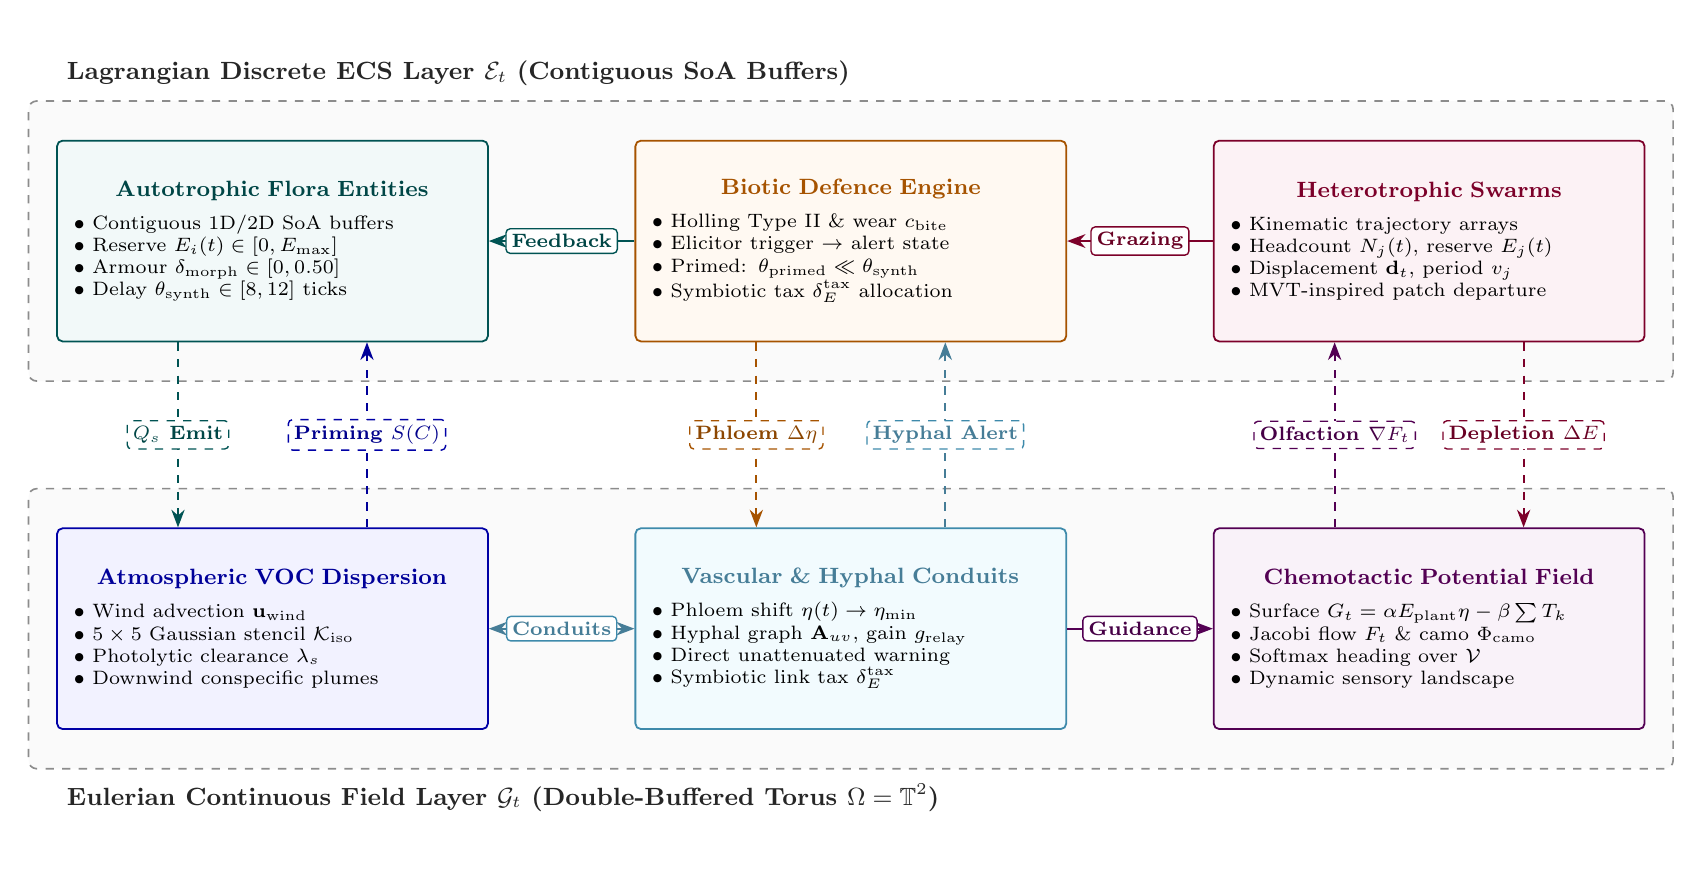
\begin{tikzpicture}[
    >=Stealth,
    font=\scriptsize,
    card/.style={draw=#1!65!black, fill=#1!5, rounded corners=2pt, line width=0.65pt, inner sep=6pt, align=left, text width=5.05cm, minimum height=2.55cm},
    layer/.style={draw=black!45, dashed, fill=black!2, rounded corners=3pt, line width=0.6pt, inner xsep=10pt, inner ysep=10pt},
    badge/.style={draw=#1!65!black, fill=white, rounded corners=1.5pt, line width=0.5pt, inner sep=2pt, font=\scriptsize\bfseries, text=#1!55!black}
  ]

  % Top Layer: Discrete ECS Cards
  \node[card=teal] (flora) {%
    \centering\textbf{\footnotesize\color{teal!55!black}Autotrophic Flora Entities}\\[4pt]
    \raggedright
    $\bullet$ Contiguous 1D/2D SoA buffers\\
    $\bullet$ Reserve $E_i(t) \in [0, E_{\max}]$\\
    $\bullet$ Armour $\delta_{\mathrm{morph}} \in [0, 0.50]$\\
    $\bullet$ Delay $\theta_{\mathrm{synth}} \in [8, 12]$ ticks%
  };

  \node[card=orange, right=1.85cm of flora] (def) {%
    \centering\textbf{\footnotesize\color{orange!65!black}Biotic Defence Engine}\\[4pt]
    \raggedright
    $\bullet$ Holling Type~II \& wear $c_{\mathrm{bite}}$\\
    $\bullet$ Elicitor trigger $\to$ alert state\\
    $\bullet$ Primed: $\theta_{\mathrm{primed}} \ll \theta_{\mathrm{synth}}$\\
    $\bullet$ Symbiotic tax $\delta_E^{\mathrm{tax}}$ allocation%
  };

  \node[card=purple, right=1.85cm of def] (herb) {%
    \centering\textbf{\footnotesize\color{purple!65!black}Heterotrophic Swarms}\\[4pt]
    \raggedright
    $\bullet$ Kinematic trajectory arrays\\
    $\bullet$ Headcount $N_j(t)$, reserve $E_j(t)$\\
    $\bullet$ Displacement $\mathbf{d}_t$, period $v_j$\\
    $\bullet$ MVT-inspired patch departure%
  };

  % Bottom Layer: Continuous Eulerian Cards (ample vertical gap for conduits & Layer 2 label)
  \node[card=blue, below=2.35cm of flora] (voc) {%
    \centering\textbf{\footnotesize\color{blue!60!black}Atmospheric VOC Dispersion}\\[4pt]
    \raggedright
    $\bullet$ Wind advection $\mathbf{u}_{\mathrm{wind}}$\\
    $\bullet$ $5 \times 5$ Gaussian stencil $\mathcal{K}_{\mathrm{iso}}$\\
    $\bullet$ Photolytic clearance $\lambda_s$\\
    $\bullet$ Downwind conspecific plumes%
  };

  \node[card=cyan, below=2.35cm of def] (myco) {%
    \centering\textbf{\footnotesize\color{cyan!55!black}Vascular \& Hyphal Conduits}\\[4pt]
    \raggedright
    $\bullet$ Phloem shift $\eta(t) \to \eta_{\min}$\\
    $\bullet$ Hyphal graph $\mathbf{A}_{uv}$, gain $g_{\mathrm{relay}}$\\
    $\bullet$ Direct unattenuated warning\\
    $\bullet$ Symbiotic link tax $\delta_E^{\mathrm{tax}}$%
  };

  \node[card=violet, below=2.35cm of herb] (chemo) {%
    \centering\textbf{\footnotesize\color{violet!65!black}Chemotactic Potential Field}\\[4pt]
    \raggedright
    $\bullet$ Surface $G_t = \alpha E_{\mathrm{plant}}\eta - \beta\sum T_k$\\
    $\bullet$ Jacobi flow $F_t$ \& camo $\Phi_{\mathrm{camo}}$\\
    $\bullet$ Softmax heading over $\mathcal{V}$\\
    $\bullet$ Dynamic sensory landscape%
  };

  % Outer layer frames via background
  \begin{scope}[on background layer]
    \node[layer, fit=(flora)(def)(herb), inner ysep=14pt] (L1) {};
    \node[layer, fit=(voc)(myco)(chemo), inner ysep=14pt] (L2) {};
  \end{scope}

  % Explicit foreground layer titles positioned clearly outside/above and below frame borders
  \node[fill=white, anchor=south west, font=\small\bfseries, text=black!85, inner xsep=4pt, inner ysep=2pt] (L1_lbl) at ([xshift=10pt, yshift=3pt]L1.north west) {Lagrangian Discrete ECS Layer $\mathcal{E}_t$ (Contiguous SoA Buffers)};
  \node[fill=white, anchor=north west, font=\small\bfseries, text=black!85, inner xsep=4pt, inner ysep=2pt] (L2_lbl) at ([xshift=10pt, yshift=-3pt]L2.south west) {Eulerian Continuous Field Layer $\mathcal{G}_t$ (Double-Buffered Torus $\Omega = \mathbb{T}^2$)};

  % Intra-layer horizontal arrows
  \draw[->, line width=0.8pt, color=purple!65!black] (herb.west) -- node[badge=purple] {Grazing} (def.east);
  \draw[->, line width=0.8pt, color=teal!65!black] (def.west) -- node[badge=teal] {Feedback} (flora.east);
  \draw[<->, line width=0.8pt, color=cyan!55!black] (voc.east) -- node[badge=cyan] {Conduits} (myco.west);
  \draw[->, line width=0.8pt, color=violet!65!black] (myco.east) -- node[badge=violet] {Guidance} (chemo.west);

  % Inter-layer vertical coupling arrows cleanly separated in the 2.35cm middle corridor
  \draw[->, dashed, line width=0.75pt, color=teal!65!black] ([xshift=-1.2cm]flora.south) -- node[badge=teal] {$Q_s$ Emit} ([xshift=-1.2cm]voc.north);
  \draw[->, dashed, line width=0.75pt, color=blue!60!black] ([xshift=1.2cm]voc.north) -- node[badge=blue] {Priming $S(C)$} ([xshift=1.2cm]flora.south);

  \draw[->, dashed, line width=0.75pt, color=orange!65!black] ([xshift=-1.2cm]def.south) -- node[badge=orange] {Phloem $\Delta\eta$} ([xshift=-1.2cm]myco.north);
  \draw[->, dashed, line width=0.75pt, color=cyan!55!black] ([xshift=1.2cm]myco.north) -- node[badge=cyan] {Hyphal Alert} ([xshift=1.2cm]def.south);

  \draw[->, dashed, line width=0.75pt, color=violet!65!black] ([xshift=-1.2cm]chemo.north) -- node[badge=violet] {Olfaction $\nabla F_t$} ([xshift=-1.2cm]herb.south);
  \draw[->, dashed, line width=0.75pt, color=purple!65!black] ([xshift=1.2cm]herb.south) -- node[badge=purple] {Depletion $\Delta E$} ([xshift=1.2cm]chemo.north);

  % Explicit vertical padding so outer north/south layer headers never clip
  \path ([yshift=10pt]current bounding box.north) ([yshift=-10pt]current bounding box.south);
\end{tikzpicture}
}

  \caption{The Coupled Hybrid Dynamical Architecture of PHIDS. Discrete biological entities stored in the data-oriented Entity--Component--System (ECS) layer $\mathcal{E}_t$ interact via localised grazing and damage triggers, sourcing continuous chemical concentration fields $C_s$ and guidance potentials $F_t$ evaluated across double-buffered cellular layers $\mathcal{G}_t$ on a toroidal topology $\mathbb{T}^2$.}
  \label{fig:architectural_paradigm}
\end{figure*}

\subsection{Coupled Hybrid Architecture}
\label{sec:intro_architectural_vision}

To combine spatial--biochemical detail with predictable execution throughput, we present \textbf{PHIDS} (Plant--Herbivore Interaction \& Defence Simulator). Extending our earlier discrete-event prototype \cite{dietrich2025visual}, PHIDS implements a coupled hybrid dynamical system \cite{swat2012multiscale, topping2003almass, bravo2020hybrid, husar2024mcell4} partitioned into two synchronised layers (Fig.~\ref{fig:architectural_paradigm}):
\begin{enumerate}
  \item \textbf{Discrete Lagrangian Entity Layer ($\mathcal{E}_t$):} Sessile plants and mobile herbivore swarms reside in a data-oriented Entity--Component--System (ECS) backed by contiguous Structure-of-Arrays (SoA) memory buffers \cite{lam2015numba, harris2020array}, avoiding per-organism pointer chasing and supporting $\mathcal{O}(1)$ spatial lookups.
  \item \textbf{Continuous Eulerian Field Layer ($\mathcal{G}_t$):} Semiochemicals, volatile concentrations, and sensory fields are stored as 2D scalar arrays on a periodic toroidal lattice $\Omega = \mathbb{T}^2$. Airborne transport evolves via operator-split Reaction--Diffusion--Advection PDEs \cite{strang1968construction, leveque2002finite}, whereas chemotactic navigation potentials are computed via compiled Jacobi iterative relaxation kernels \cite{lam2015numba}.
\end{enumerate}

By coupling discrete agent transitions with continuous field operators at hourly resolution, PHIDS resolves Holling Type~II intake saturation \cite{holling1959components}, an MVT-inspired local patch-departure heuristic \cite{charnov1976optimal}, sigmoidal Hill receptor priming, and vascular phloem withdrawal \cite{schwachtje2006snf1} across tens of thousands of interacting organisms.

\subsection{Structural Homomorphism to Distributed WSN Security}
\label{sec:intro_wsn_paradigm}

Beyond spatial systems biology, the dynamical architecture of PHIDS shares a formal structural homomorphism and computational Design Space Exploration (DSE) methodology with distributed resilience planning in large-scale static Wireless Sensor Networks (WSNs) \cite{forster2023novel, forster2024determining, forster2024topology, dressler2010survey}. Static sensor deployments face a parallel energy-allocation trade-off to sessile flora (Table~\ref{tab:energetic_allocation_tradeoffs}): continuous cryptographic checks deplete constrained battery reserves, whereas passive sleep states expose networks to multi-hop disruption during activation delays \cite{forster2023novel, forster2024determining}. Building on our prior WSN security and EEDSE work \cite{forster2023novel, forster2024determining, forster2024topology, dietrich2025visual}, Section~\ref{sec:wsn_isomorphism} formalises this structural mapping --- including explicit non-isomorphism boundaries --- and transfers the multi-fidelity calibration, sensitivity screening, and deterministic SoA workflows across both domains.

\begin{table*}[b]
  \centering
  \caption{Energetic Allocation Trade-offs Across Autotrophic Phenotypic Strategies in Meso-Scale Biotopes.}
  \label{tab:energetic_allocation_tradeoffs}
  % ==============================================================================
% Table 1: Energetic Allocation Trade-offs Across Autotrophic Phenotypes
% Placed at [b] (bottom of page)
% ==============================================================================

\footnotesize
\renewcommand{\arraystretch}{1.15}
\begin{tabularx}{\textwidth}{
  >{\raggedright\arraybackslash\hsize=0.85\hsize}X
  >{\centering\arraybackslash\hsize=0.70\hsize}X
  >{\centering\arraybackslash\hsize=0.68\hsize}X
  >{\centering\arraybackslash\hsize=0.68\hsize}X
  >{\raggedright\arraybackslash\hsize=0.74\hsize}X
  >{\raggedright\arraybackslash\hsize=0.85\hsize}X
  >{\raggedright\arraybackslash\hsize=1.50\hsize}X
}
  \toprule
  \textbf{Plant Phenotype Class} &
  \textbf{Vegetative Growth} ($g_j$) &
  \textbf{Morph. Upkeep} ($\delta_{\text{morph}}$) &
  \textbf{Inducible Defence} ($\delta_{\text{chem}}$) &
  \textbf{Signalling Channel} &
  \textbf{Target Herbivore Guild} &
  \textbf{Ecological Strategy} \\
  \midrule
  \textbf{Pioneer Autotroph} &
  High ($85$--$95\%$) &
  Negligible ($0$--$2\%$) &
  Zero ($0\%$) &
  None &
  Generalist Foliivores &
  Rapid spatial colonisation prioritising reproductive output over individual tissue protection. \\
  \addlinespace[3pt]
  \textbf{Constitutive Armoured} &
  Low ($20$--$35\%$) &
  High ($30$--$50\%$) &
  Low ($5$--$10\%$) &
  Passive Airborne &
  Chewing Macrobrowsers &
  Static physical hardening paying sustained maintenance costs for zero-latency protection. \\
  \addlinespace[3pt]
  \textbf{Inducible Synthesiser} &
  Medium ($50$--$65\%$) &
  Low ($5$--$10\%$) &
  High ($25$--$40\%$) &
  Airborne VOC Plumes &
  Specialist Swarms &
  On-demand allelochemical synthesis, vulnerable during countdown latency $\theta_{\text{synth}}$ unless primed. \\
  \addlinespace[3pt]
  \textbf{Symbiotic Networker} &
  Medium ($45$--$60\%$) &
  Low ($5$--$10\%$) &
  Medium ($20$--$30\%$) &
  Subterranean Hyphae &
  Invasive Phloem Feeders &
  Maintains persistent CMN conduits at carbon tax $\delta_E^{\text{tax}}$ to sustain wind-independent local warnings. \\
  \bottomrule
\end{tabularx}

\end{table*}

\subsection{Summary of Contributions}
\label{sec:intro_contributions}

The contributions of this work are fourfold:
\begin{enumerate}
  \item \textbf{Coupled Hybrid Simulator Architecture:} A data-oriented SoA Entity--Component--System paired with operator-split 2D reaction--diffusion--advection PDEs, Jacobi flow relaxation, and dynamic cardinal root graphs, compiled to LLVM native kernels with bit-exact thread determinism and Zarr compression (Section~\ref{sec:computational_realisation}).
  \item \textbf{Multi-Channel Botanical Defence Kinetics:} Parameterised operational equations for constitutive armour, structural tissue upkeep, airborne volatile dispersion, Hill receptor priming, subterranean mycorrhizal relays, and phloem palatability withdrawal.
  \item \textbf{Analytical System Bounds:} Three analytical propositions establishing carrying-capacity boundedness and non-reproductive dissipation, the closed-form continuous-grazing critical synthesis delay $\theta_{\text{crit}}$, and a mean-field delay-bifurcation criterion ($\tau^* = 2.38\,\text{h} > 1.0\,\text{h}$), checked against empirical cross-thread invariance.
  \item \textbf{In-Silico Case Studies and Structural DSE Mapping:} Evaluation on a $256 \times 256$ Central European ecotone spanning multi-fidelity Bayesian calibration, $10$-seed single-season zero-shot transfer, continuous-vs-diurnal bound diagnostics, $90$-run dual-channel wind ablations ($+21$-run upwind relay), and $1{,}792 + 224$-run CRN Sobol sensitivity analyses alongside formal structural mapping to static WSN DSE pipelines.
\end{enumerate}

\subsection{Article Organisation}
\label{sec:intro_organization}

Section~\ref{sec:biological_domain} introduces the biological defence tiers and foraging kinematics, and Section~\ref{sec:related_works} positions PHIDS relative to existing simulation frameworks. Section~\ref{sec:mathematical_framework} formulates the coupled hybrid mathematical model, Section~\ref{sec:theoretical_invariants} derives the analytical bounds and stability properties, and Section~\ref{sec:case_studies} evaluates the framework on the Central European ecotone. Section~\ref{sec:computational_realisation} details the ECS memory layout, JIT kernel design, Roofline scaling, double-buffered determinism, and Zarr replay storage; Section~\ref{sec:discussion} synthesises ecological buffering, the structural WSN homomorphism and DSE transfer, and model assumptions; and Section~\ref{sec:conclusion} concludes.


% ==============================================================================
% Section 2: The Biological Problem Domain & Botanical Defence Kinetics
% ==============================================================================
% ==============================================================================
% Section 2: The Biological Problem Domain & Botanical Defence Kinetics
% ==============================================================================

\section{Biological Problem Domain and Defence Kinetics}
\label{sec:biological_domain}

\begin{figure*}[t]
  \centering
  % ==============================================================================
% Figure 2: Botanical Defence Cascade (Native TikZ/PGF)
% ==============================================================================

\resizebox{0.96\textwidth}{!}{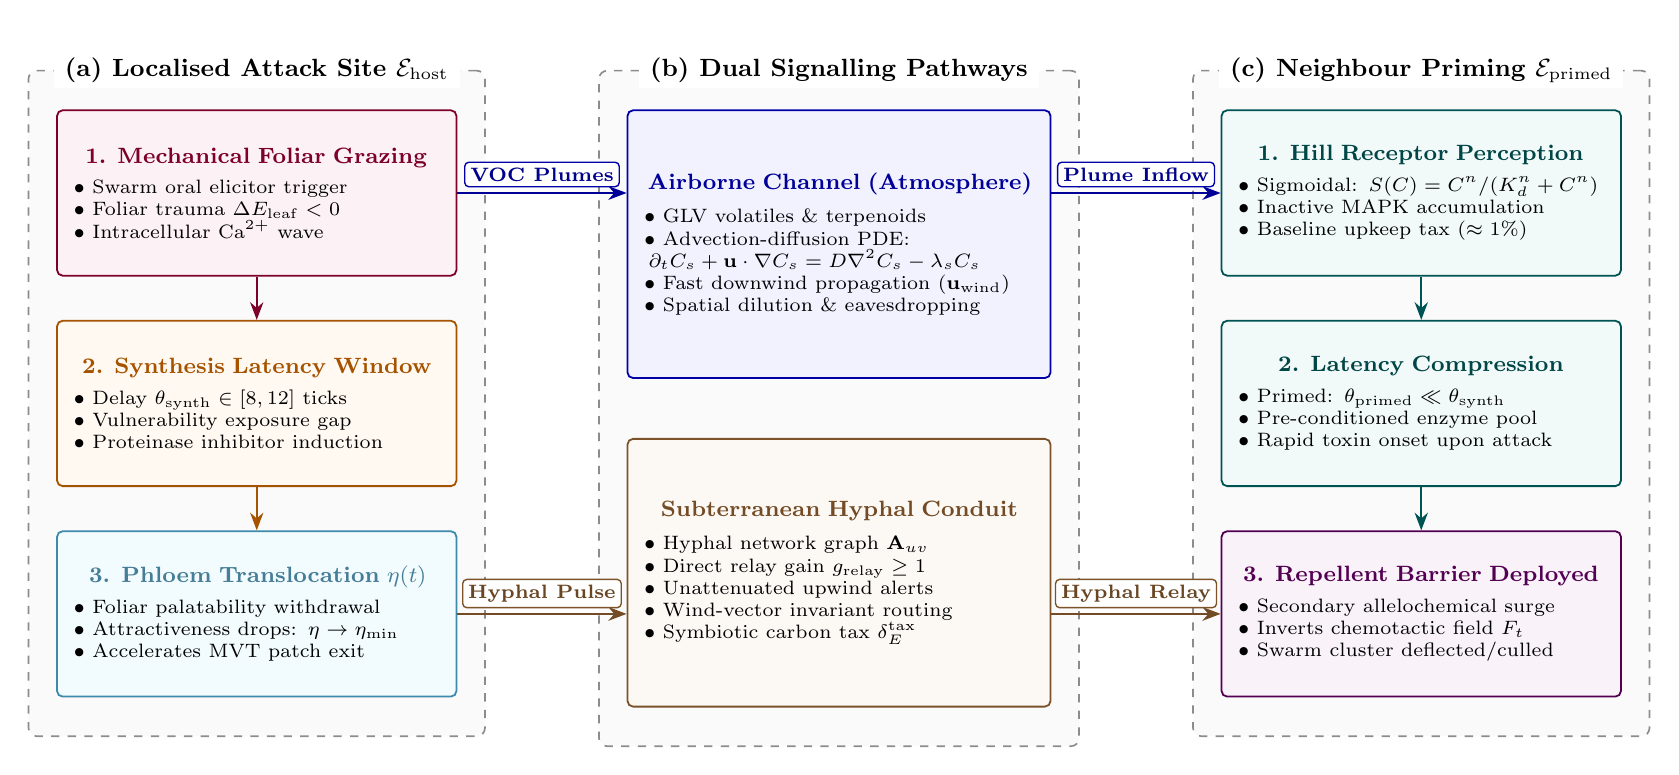
\begin{tikzpicture}[
    >=Stealth,
    font=\scriptsize,
    card/.style={draw=#1!65!black, fill=#1!5, rounded corners=2pt, line width=0.65pt, inner sep=6pt, align=left, text width=4.65cm, minimum height=2.1cm},
    tallcard/.style={draw=#1!65!black, fill=#1!5, rounded corners=2pt, line width=0.65pt, inner sep=6pt, align=left, text width=4.95cm, minimum height=3.4cm},
    panel/.style={draw=black!45, dashed, fill=black!2, rounded corners=3pt, line width=0.6pt, inner sep=10pt},
    badge/.style={draw=#1!65!black, fill=white, rounded corners=1.5pt, line width=0.5pt, inner sep=2pt, font=\scriptsize\bfseries, text=#1!55!black}
  ]

  % Panel (a) Attack site stacked cleanly with relative positioning
  \node[card=purple] (a1) {%
    \centering\textbf{\footnotesize\color{purple!65!black}1. Mechanical Foliar Grazing}\\[3pt]
    \raggedright
    $\bullet$ Swarm oral elicitor trigger\\
    $\bullet$ Foliar trauma $\Delta E_{\mathrm{leaf}} < 0$\\
    $\bullet$ Intracellular $\mathrm{Ca}^{2+}$ wave%
  };
  \node[card=orange, below=0.55cm of a1] (a2) {%
    \centering\textbf{\footnotesize\color{orange!65!black}2. Synthesis Latency Window}\\[3pt]
    \raggedright
    $\bullet$ Delay $\theta_{\mathrm{synth}} \in [8, 12]$ ticks\\
    $\bullet$ Vulnerability exposure gap\\
    $\bullet$ Proteinase inhibitor induction%
  };
  \node[card=cyan, below=0.55cm of a2] (a3) {%
    \centering\textbf{\footnotesize\color{cyan!55!black}3. Phloem Translocation $\eta(t)$}\\[3pt]
    \raggedright
    $\bullet$ Foliar palatability withdrawal\\
    $\bullet$ Attractiveness drops: $\eta \to \eta_{\min}$\\
    $\bullet$ Accelerates MVT patch exit%
  };
  \draw[->, line width=0.75pt, color=purple!65!black] (a1.south) -- (a2.north);
  \draw[->, line width=0.75pt, color=orange!65!black] (a2.south) -- (a3.north);

  % Panel (b) Dual Signalling Pathways (ample horizontal corridor 2.15cm for arrow badges)
  \node[tallcard=blue, right=2.15cm of a1, anchor=north west, yshift=0cm] (b1) at (a1.north east) {%
    \centering\textbf{\footnotesize\color{blue!60!black}Airborne Channel (Atmosphere)}\\[4pt]
    \raggedright
    $\bullet$ GLV volatiles \& terpenoids\\
    $\bullet$ Advection-diffusion PDE:\\
    \hspace*{0.2em}$\partial_t C_s + \mathbf{u}\cdot\nabla C_s = D\nabla^2 C_s - \lambda_s C_s$\\
    $\bullet$ Fast downwind propagation ($\mathbf{u}_{\mathrm{wind}}$)\\
    $\bullet$ Spatial dilution \& eavesdropping%
  };
  \node[tallcard=brown, below=0.75cm of b1] (b2) {%
    \centering\textbf{\footnotesize\color{brown!60!black}Subterranean Hyphal Conduit}\\[4pt]
    \raggedright
    $\bullet$ Hyphal network graph $\mathbf{A}_{uv}$\\
    $\bullet$ Direct relay gain $g_{\mathrm{relay}} \ge 1$\\
    $\bullet$ Unattenuated upwind alerts\\
    $\bullet$ Wind-vector invariant routing\\
    $\bullet$ Symbiotic carbon tax $\delta_E^{\mathrm{tax}}$%
  };

  % Panel (c) Neighbour Priming (ample horizontal corridor 2.15cm)
  \node[card=teal, right=2.15cm of b1.north east, anchor=north west] (c1) {%
    \centering\textbf{\footnotesize\color{teal!55!black}1. Hill Receptor Perception}\\[3pt]
    \raggedright
    $\bullet$ Sigmoidal: $S(C) = C^n / (K_d^n + C^n)$\\
    $\bullet$ Inactive MAPK accumulation\\
    $\bullet$ Baseline upkeep tax ($\approx 1\%$)%
  };
  \node[card=teal, below=0.55cm of c1] (c2) {%
    \centering\textbf{\footnotesize\color{teal!55!black}2. Latency Compression}\\[3pt]
    \raggedright
    $\bullet$ Primed: $\theta_{\mathrm{primed}} \ll \theta_{\mathrm{synth}}$\\
    $\bullet$ Pre-conditioned enzyme pool\\
    $\bullet$ Rapid toxin onset upon attack%
  };
  \node[card=violet, below=0.55cm of c2] (c3) {%
    \centering\textbf{\footnotesize\color{violet!65!black}3. Repellent Barrier Deployed}\\[3pt]
    \raggedright
    $\bullet$ Secondary allelochemical surge\\
    $\bullet$ Inverts chemotactic field $F_t$\\
    $\bullet$ Swarm cluster deflected/culled%
  };
  \draw[->, line width=0.75pt, color=teal!65!black] (c1.south) -- (c2.north);
  \draw[->, line width=0.75pt, color=teal!65!black] (c2.south) -- (c3.north);

  \begin{scope}[on background layer]
    \node[panel, fit=(a1)(a3), inner ysep=14pt] (pa) {};
    \node[panel, fit=(b1)(b2), inner ysep=14pt] (pb) {};
    \node[panel, fit=(c1)(c3), inner ysep=14pt] (pc) {};
  \end{scope}

  \node[fill=white, anchor=center, font=\small\bfseries, inner xsep=4pt, inner ysep=2pt] (pa_lbl) at (pa.north) {(a) Localised Attack Site $\mathcal{E}_{\mathrm{host}}$};
  \node[fill=white, anchor=center, font=\small\bfseries, inner xsep=4pt, inner ysep=2pt] (pb_lbl) at (pb.north) {(b) Dual Signalling Pathways};
  \node[fill=white, anchor=center, font=\small\bfseries, inner xsep=4pt, inner ysep=2pt] (pc_lbl) at (pc.north) {(c) Neighbour Priming $\mathcal{E}_{\mathrm{primed}}$};

  % Inter-panel horizontal conduits with centred pills inside the 2.15cm gap
  \draw[->, line width=0.8pt, color=blue!60!black] (a1.east) -- node[above=2pt, badge=blue] {VOC Plumes} (b1.west |- a1.east);
  \draw[->, line width=0.8pt, color=blue!60!black] (b1.east |- c1.west) -- node[above=2pt, badge=blue] {Plume Inflow} (c1.west);
  \draw[->, line width=0.8pt, color=brown!60!black] (a3.east) -- node[above=2pt, badge=brown] {Hyphal Pulse} (b2.west |- a3.east);
  \draw[->, line width=0.8pt, color=brown!60!black] (b2.east |- c3.west) -- node[above=2pt, badge=brown] {Hyphal Relay} (c3.west);

  % Explicit top padding so above-panel titles never clip
  \path ([yshift=0.30cm]pa_lbl.north) ([yshift=0.30cm]pb_lbl.north) ([yshift=0.30cm]pc_lbl.north);
\end{tikzpicture}
}

  \caption{Multi-Layer Botanical Defence Hierarchy and Dual-Channel Communication Cascades. Attacked plants activate localised induced defences while transmitting airborne VOC plumes and subterranean mycorrhizal signals to prime both downwind neighbours (via airborne VOCs) and upwind or adjacent cardinal neighbours (via subterranean CMNs), simultaneously withdrawing mobile phloem nutrients to reduce palatability.}
  \label{fig:botanical_defense_hierarchy}
\end{figure*}

Terrestrial plant communities persist through layered morphological, biochemical, and vascular defences \cite{gatehouse2002plant}. Incapable of fleeing foraging herbivores, plants partition photosynthetic energy between somatic vegetative growth and defensive barriers \cite{charnov1976optimal, gatehouse2002plant}. Classical Lotka--Volterra formulations \cite{lotka1925elements, volterra1926fluctuations} treat plant susceptibility as a static scalar, obscuring non-linear synthesis delays, spatial refugia, and dual-channel warning cascades. Below we introduce the conceptual physiological abstractions for the five biological mechanisms implemented in PHIDS; their exact discrete operational recurrences and conservation laws are formalised in Section~\ref{sec:mathematical_framework} (Section~\ref{subsec:trophic_kinetics}).

\subsection{Botanical Defence Hierarchy}
\label{subsec:defense_hierarchy}

Autotrophic defences operate across three functional tiers (Fig.~\ref{fig:botanical_defense_hierarchy}). First, constitutive morphological defences -- lignified cell walls, glandular trichomes, epidermal waxes, and biogenic silica phytoliths -- are built permanently into mature tissue \cite{gatehouse2002plant}. Conceptually, they represent a sunken structural allocation:
\begin{equation}
  E_{\text{somatic}} = E_{\text{total}} \cdot (1 - \delta_{\text{morph}}), \quad \delta_{\text{morph}} \in [0, 0.50],
\end{equation}
where $\delta_{\text{morph}}$ denotes the effective fraction by which physical reinforcement attenuates digestibility, complemented in discrete cohorts by structural tissue accretion and maintenance (Eq.~\eqref{eq:structural_mass_growth}).

Second, inducible chemical defences remain metabolically inactive at rest and are synthesised \textit{de novo} only after mechanical wounding or herbivore oral elicitors \cite{gatehouse2002plant}. Conceptually, foliar energy balance follows:
\begin{equation}
  \frac{\mathrm{d}E_{\text{reserve}}}{\mathrm{d}t} = P_i(t) - R_{\text{maint}} - \mathbb{I}_{\text{induced}} \cdot C_{\text{synth}},
\end{equation}
where $P_i(t)$ represents photosynthetic intake, $R_{\text{maint}}$ structural maintenance respiration, $\mathbb{I}_{\text{induced}} \in \{0, 1\}$ the active induction indicator, and $C_{\text{synth}}$ enzymatic synthesis expenditure (realised discretely per tick and weekly cohort in Section~\ref{subsec:trophic_kinetics}).

Third, physiological priming bridges constitutive and inducible strategies \cite{farmer2001surface, baldwin2006volatile, babikova2013underground, arimura2025cracking}. Detecting low-level airborne or subterranean cues from damaged neighbours places an unattacked plant in a primed alert state without immediate investment in full toxin synthesis. Primed tissues accumulate cytosolic calcium ($\text{Ca}^{2+}$) transients \cite{aratani2023green}, inactive mitogen-activated protein kinases (MAPKs), and chromatin marks on jasmonate-responsive promoters \cite{gatehouse2002plant, arimura2025cracking} at minor energetic cost ($\approx 1\%$ of baseline reserve), enabling rapid toxin deployment upon subsequent grazing.

\subsection{Dual-Channel Communication Networks}
\label{subsec:communication_networks}

Sessile flora exchange stress cues across two contrasting physical media (Fig.~\ref{fig:botanical_defense_hierarchy}). In the atmospheric channel, foliar wounding releases green leaf volatiles such as $(Z)$-3-hexenal and $(E)$-2-hexenal together with terpenoids including $(E)$-$\beta$-ocimene and $(E)$-4,8-dimethyl-1,3,7-nonatriene \cite{farmer2001surface, baldwin2006volatile, aratani2023green}. Wind advection and turbulent diffusion carry these plumes rapidly downwind \cite{okubo2001diffusion}, yet airborne warning suffers three structural constraints:
\begin{enumerate}
  \item \textbf{Directional Asymmetry:} Plumes travel downwind along $\mathbf{u}_{\text{wind}}$, leaving upwind and crosswind plants unwarned.
  \item \textbf{Atmospheric Dilution:} Airborne concentration $C_{\text{voc}}(\mathbf{x}, t)$ attenuates via advection, dispersion, and photolytic clearance (Section~\ref{subsec:atmospheric_transport}, Eq.~\ref{eq:reaction_diffusion_pde}).
  \item \textbf{Herbivore Eavesdropping:} Specialised herbivores exploit unencrypted VOC gradients as chemotactic beacons toward stressed hosts \cite{baldwin2006volatile, arimura2025cracking}.
\end{enumerate}

To compensate for directional wind asymmetry, plants form subterranean common mycelial networks (CMNs) linking adjacent root systems \cite{babikova2013underground}. Upon elicitation, stressed hosts partition emitted warning cues between airborne plumes and a cardinal-adjacent dynamic root-link graph as formalised in Section~\ref{subsec:trophic_kinetics} (Eq.~\ref{eq:myco_neighbor_flux}) \cite{babikova2013underground}. Subterranean conduction operates independently of wind direction and atmospheric dilution, remaining hidden from foliar herbivores. Empirical syntheses, however, note that CMN maintenance imposes measurable carbon-for-nutrient costs and depends on intact hyphal topology \cite{karst2023positive, henriksson2023reexamining}. PHIDS therefore models the CMN as a metabolically taxed nearest-neighbour lattice graph requiring sustained host carbon allocation ($\delta_E^{\text{tax}} \approx 0.5\text{--}1.5\%$ of baseline reserve) \cite{babikova2013underground, henriksson2023reexamining}; interrupting this carbon supply severs hyphal links.

% ==============================================================================
% Table 2: Biochemical Parameters of Botanical Defenses and Signals
% Placed at bottom [b] of page, caption above table
% ==============================================================================
%
% NARRATIVE STORY OF TABLE 2:
% This table establishes the empirical calibration underpinning the biological
% simulation engine in PHIDS. It bridges established empirical literature in plant
% physiology and chemical ecology with the formal computational parameters used across
% the coupled hybrid system.
%
% The narrative progresses through five functional tiers of plant defence:
% 1. Constitutive Morphological Barriers: Static structures (trichomes, biogenic
%    silica, lignified secondary cell walls) that require upfront energetic allocation
%    during tissue maturation but impose zero ongoing synthesis delay upon attack.
% 2. Airborne VOC Signals (Green Leaf Volatiles & Terpenoids): Rapidly emitted semiochemical
%    plumes that diffuse through the turbulent atmospheric boundary layer to prime downwind
%    conspecifics, characterised by high dispersion and finite photochemical half-lives.
% 3. Subterranean Mycorrhizal Networks (CMNs): Underground hyphal networks that provide
%    shielded, out-of-band communication conduits connecting root systems, operating at a
%    continuous metabolic maintenance fee (carbon tax) paid by the host plant.
% 4. Inducible Allochemical Defenses (Glucosinolates, Alkaloids, Proteinase Inhibitors):
%    Metabolically expensive secondary toxins synthesized de novo upon tissue wounding,
%    subject to a critical physiological lag phase (synthesis delay theta_synth).
% 5. Vascular Phloem Translocation (Carbon/Nitrogen Sinks): Rapid enzymatic reallocation
%    of mobile sugars and amino acids away from grazed foliar tissue into subterranean root
%    storage, dynamically reducing apparent tissue nutrition factor eta(t).
%
% ==============================================================================

\begin{table*}[b]
\caption{Biochemical, Physiological, and Kinetic Parameters Governing Botanical Defence Cascades in PHIDS.}
\label{tab:biochemical_parameters}
\vspace{4pt}
\centering
\footnotesize
\begin{tabularx}{\textwidth}{
  >{\raggedright\hsize=0.90\hsize}X
  >{\raggedright\hsize=1.00\hsize}X
  >{\centering\hsize=0.95\hsize}X
  >{\centering\hsize=0.80\hsize}X
  >{\centering\hsize=0.90\hsize}X
  >{\raggedright\hsize=1.15\hsize}X
  >{\raggedright\arraybackslash\hsize=1.30\hsize}X
}
\toprule
\textbf{Defence Modality} &
\textbf{Biochemical Basis} &
\textbf{Metabolic Cost} &
\textbf{Latency ($\bm{\theta}$)} &
\textbf{Decay / Half-Life} &
\textbf{Empirical Basis} &
\textbf{Model Symbol / Role} \\
\midrule

\textbf{Constitutive Armour} &
Lignin, cellulose, silica trichomes &
Continuous fraction \newline $\delta_{\mathrm{morph}} \in [0, 0.50]$ &
$0\,\text{ticks}$ (Permanent) &
$\tau_{1/2} \to \infty$ (Permanent) &
Gatehouse \cite{gatehouse2002plant} &
$\delta_{\mathrm{morph}}$ (digestibility), \newline
$c_{\mathrm{bite}}$ (mechanical wear) \\

\textbf{Airborne VOC Plumes} &
$(E)$-$\beta$-ocimene, green leaf volatiles &
Signal emission $Q_{\mathrm{emit}}$; zero resting tax &
$1\text{--}3\,\text{ticks}$ (Plume onset) &
Clearance $\gamma_s \approx 1 - \lambda_s\Delta t$ (diffusion $\sigma = 0.40$) &
Farmer \cite{farmer2001surface} &
$Q_{\mathrm{emit}}$ (emission flux), \newline
$\gamma_s$ (clearance retention) \\

\textbf{Mycelial Conduction} &
Hyphal action potentials, jasmonates &
Link upkeep $\delta_E^{\mathrm{tax}}$ / link &
$1\,\text{tick/hop}$ ($1\text{--}3\,\text{ticks}$) &
Unattenuated across cardinal links &
Babikova et al. \cite{babikova2013underground} &
$\delta_E^{\mathrm{tax}}$ (link carbon tax), \newline
$g_{\mathrm{relay}}$ (relay gain) \\

\textbf{Inducible Toxins} &
Glucosinolates, nicotine, proteinase inhibitors &
Active synthesis tax $c_{\mathrm{synth}}$ / tick &
$8\text{--}12\,\text{ticks}$ ($1\text{--}2$ in compact orchard runs; $\theta_{\mathrm{synth}}$) &
Active persistence $\tau_{\mathrm{aft}}$ ticks &
Gatehouse \cite{gatehouse2002plant} &
$\theta_{\mathrm{synth}}$ (induction lag), \newline
$\mu_{\mathrm{tox}}$ (lethality rate) \\

\textbf{Primed Acceleration} &
Pre-transcribed mRNA, inactive enzyme pools &
$\approx 1\%$ resting alert upkeep &
$1\text{--}3\,\text{ticks}$ ($\theta_{\mathrm{primed}}$) &
Gated by Hill saturation $S(C) \ge \tau_{\mathrm{prim}}$ &
Gatehouse \cite{gatehouse2002plant} &
$n$ (Hill exponent), \newline
$K_d$ (half-saturation) \\

\textbf{Phloem Translocation} &
Apparent foliar nutrition withdrawal &
Stress withdrawal without biomass loss &
Rate-limited recovery ($\gamma_{\text{trans}}$) &
Relaxation: $\eta(t+1) = \eta(t) + \Delta \eta$ &
Schwachtje et al. \cite{schwachtje2006snf1} &
$\gamma_{\mathrm{trans}}$ (recovery rate), \newline
$\eta(t)$ (palatability factor) \\

\bottomrule
\end{tabularx}
\end{table*}


\subsection{Synthesis Latency and Vulnerability Window}
\label{subsec:latency_window}

De-novo secondary metabolite synthesis is delayed by octadecanoid signalling, transcription, ribosomal translation, and enzymatic conversion, creating a physiological latency $\theta$ \cite{gatehouse2002plant}:
\begin{equation}
  T_i(t) =
  \begin{cases}
    0, & t < t_{\text{attack}} + \theta_i, \\
    \delta_{\text{chem}} \cdot E_i(t), & t \ge t_{\text{attack}} + \theta_i,
  \end{cases}
  \label{eq:toxin_latency}
\end{equation}
where $\delta_{\text{chem}} \in [0.15, 0.40]$ is the inducible chemical investment fraction and $E_i(t)$ host reserve. Unprimed latencies span $\theta_{\text{synth}} \in [8, 12]\,\text{ticks}$ in analytical survival regimes ($6\text{--}24\,\text{h}$ in empirical physiology, scaled to $1\text{--}3\,\text{ticks}$ in high-turnover orchard benchmarks) \cite{gatehouse2002plant}, leaving unprimed hosts unprotected during initial grazing. Pre-primed neighbours accelerate toxin mobilisation to:
\begin{equation}
  \theta_{\text{primed}} = \max\left(1, \, \lfloor \theta_{\text{synth}} \cdot \kappa_{\text{prime}} \rfloor\right),
\end{equation}
with acceleration factor $\kappa_{\text{prime}} \in [0.10, 0.25]$ yielding $\theta_{\text{primed}} \in [1, 3]\,\text{ticks}$ from an $8\text{--}12\,\text{tick}$ baseline -- a $75\text{--}90\%$ latency compression.

\subsection{Phloem Vascular Resource Reallocation}
\label{subsec:phloem_translocation}

Beyond direct toxicity, grazed plants activate SNF1-related protein kinases (e.g. SnRK1) to translocate mobile sucrose and amino acids through phloem sieve elements into root parenchyma (Table~\ref{tab:biochemical_parameters}) \cite{schwachtje2006snf1}. To avoid tracking a separate subterranean biomass compartment, PHIDS models this translocation phenomenologically through a bounded foliar palatability factor $\eta_i(t) \in [\eta_{\min}, 1.0]$. Under intact conditions $\eta_i = 1.0$; grazing depresses apparent nutrition towards $\eta_{\text{target}} \ge \eta_{\min}$ before asymptotic post-grazing recovery via Eq.~\eqref{eq:phloem_recovery_recurrence} (Section~\ref{subsec:trophic_kinetics}). Lowering $\eta_i(t)$ reduces foliar attractiveness in the chemotactic field without destroying structural mass ($M_{\text{structural}}$), accelerating patch abandonment by foraging herbivores.

\subsection{Herbivore Swarm Kinematics}
\label{subsec:herbivore_kinematics}

Herbivores are modelled as discrete Lagrangian larval or wingless-colony foraging aggregations $\mathcal{E}_{\text{herb}}$ \cite{okubo2001diffusion, topping2003almass}, moving via an integer step period $v_j \in \mathbb{N}^+$ (giving step cadences $1/v_j \in \{0.33, 0.50, 1.00\}\,\text{cells/h}$; Section~\ref{subsec:swarm_kinematics}). Caloric extraction follows Holling's Type~II functional response \cite{holling1959components} (Eq.~\eqref{eq:math_holling_type_ii}), scaled post-intake by constitutive digestibility $(1 - \delta_{\mathrm{morph}, i})$ and assimilation efficiency $e_{\mathrm{eff}}$, whereas active host toxins ($T_i(t) > 0$) inflict mortality or forced dispersal. For navigation, swarms sample the chemotactic flow field $F_t(x, y)$ across their 5-cell von Neumann neighbourhood $\mathcal{V}(x, y)$ (Sections~\ref{subsec:chemotactic_potential}--\ref{subsec:swarm_kinematics}) using Boltzmann softmax selection (Eq.~\eqref{eq:boltzmann_softmax}) and a $10:1$ forward heading weight on vanishing gradients.

Patch departure follows an $\mathcal{O}(1)$ local logistic heuristic inspired by Charnov's Marginal Value Theorem (MVT) \cite{charnov1976optimal}: departure probability rises smoothly via the intake-to-upkeep ratio $\mathcal{R}_{\text{intake}} = \Delta E_{\text{consumed}} / E_{\text{upkeep}}$ (Eq.~\ref{eq:mvt_logistic_departure}), avoiding global habitat reductions. Each swarm maintains an internal caloric reserve $E_{\text{swarm}, j}(t)$ decremented by basal upkeep $U_j$ per diurnal cycle; reserves above $E_{\text{split}}$ trigger binary fission into two child swarms of size $N_j / 2$, whereas depletion below zero causes starvation mortality and ECS removal.


% ==============================================================================
% Section 3: Related Works & Methodological Benchmarking
% ==============================================================================
% ==============================================================================
% Section 3: Related Works & Methodological Benchmarking
% ==============================================================================

\section{Related Works and Methodological Benchmarking}
\label{sec:related_works}

Computational models of ecosystem dynamics, plant physiology, and consumer--resource interactions have historically developed within separate scale regimes \cite{okubo2001diffusion, swat2012multiscale}. Existing platforms generally target either regional biogeochemical crop balances, coarse-grained landscape wildlife populations, or sub-cellular tissue morphogenesis. Table~\ref{tab:simulator_benchmarking} positions PHIDS relative to these frameworks across spatial resolution, PDE transport capability, and execution throughput.

\subsection{Continuous Macro Biogeochemical Models}
\label{sec:related_biogeochem}

At landscape and regional scales ($> 100\,\text{m}$), computational agronomy and forestry rely on biogeochemical suites such as SIMPLACE \cite{enders2023simplace}, MONICA \cite{nendel2011monica}, and LANDIS-II \cite{scheller2007landis}. These tools forecast crop yields, soil water transport, and carbon--nitrogen turnover using one-dimensional vertical soil columns solving Richards water percolation and Century/RothC-style mineralisation ODEs. Although well validated for abiotic crop--soil budgets, they operate without autonomous foraging agents (reducing herbivory to exogenous defoliation scalars), resolve only daily $\Delta t = 24\,\text{h}$ steps too coarse for $1\text{--}3\,\text{h}$ plume dispersion and taxis, and exclude horizontal 2D reaction--diffusion--advection PDE solvers.

\subsection{Agent-Based Landscape and Trophic Frameworks}
\label{sec:related_abm}

Spatially explicit Agent-Based Models (ABMs) and Individual-Based Models (IBMs) capture individual movement over heterogeneous habitat maps, exemplified by ALMaSS (Animal, Landscape and Man Simulation System) \cite{topping2003almass}. ALMaSS simulates wildlife demography and pesticide exposure via procedural state machines over GIS rasters. At densities of $10^4\text{--}10^5$ interacting plants and insect swarms, however, traditional object-oriented ABMs incur pointer chasing and cache misses across scattered heap instances, and ALMaSS relies on static or piecewise-constant environmental rasters without coupled continuous semiochemical PDE solvers. General-purpose frameworks such as NetLogo \cite{wilensky1999netlogo} and Mesa \cite{kazil2020mesa} are treated separately from Table~\ref{tab:simulator_benchmarking} because they are unspecialised programming toolkits lacking built-in biophysical PDE solvers, calibrated kinetic modules, or contiguous SoA memory layouts.

\subsection{Cellular Biophysics Simulators}
\label{sec:related_cpm}

At microscopic tissue scales ($1\text{--}100\,\mu\text{m}$), hybrid continuous--discrete simulators such as CompuCell3D (CC3D) \cite{swat2012multiscale}, the Hybrid Automata Library (HAL) \cite{bravo2020hybrid}, and MCell4 \cite{husar2024mcell4} couple lattice automata or molecular Brownian particles with continuum reaction--diffusion PDEs for morphogenesis and tumour biology. In CC3D, cells span many lattice pixels evolved via Monte Carlo Step spin flips under a global Hamiltonian:
\begin{equation}
  \mathcal{H} = \sum_{\text{interfaces}} J(\tau(\sigma_i), \tau(\sigma_j)) + \sum_{\text{cells}} \lambda_{\text{vol}} (v_\sigma - V_t)^2,
  \label{eq:cc3d_hamiltonian}
\end{equation}
where $J(\tau(\sigma_i), \tau(\sigma_j))$ is interfacial contact energy, $\lambda_{\text{vol}}$ volume elasticity, $v_\sigma$ cell volume, and $V_t$ target volume. Because computational effort is dominated by sub-cellular boundary fluctuations or molecular collisions, these frameworks do not scale directly to meso-scale ecosystems requiring foraging momentum, multi-rate diurnal/weekly strides, and dual airborne--mycorrhizal signalling.

\begin{table*}[b]
  \centering
  \caption{Methodological Comparison Across Domain-Specific Ecological and Biophysical Simulation Architectures.}
  \label{tab:simulator_benchmarking}
  % ==============================================================================
% Table 4: Comprehensive Methodological Comparison Across Simulators
% Placed at [b] (bottom of page)
% Narrative Story:
% This table systematically justifies the architectural necessity of PHIDS against
% established ecological, agronomic, and biophysical simulation platforms.
% It illustrates the historical compromise: existing tools either model regional
% crop yields without biotic predators (SIMPLACE, MONICA), landscape succession
% without reactive semiochemical transport (LANDIS-II, ALMaSS), or micro-scale
% tissue morphogenesis without macroscopic animals (CompuCell3D).
% Blank-canvas toolkits (NetLogo, Mesa) are excluded from the comparison matrix
% because their unspecialized nature produces uninformative "User-Defined" entries.
% ==============================================================================

\scriptsize
\renewcommand{\arraystretch}{1.18}
\begin{tabularx}{\textwidth}{
  >{\raggedright\arraybackslash\hsize=1.05\hsize}X
  >{\raggedright\arraybackslash\hsize=1.15\hsize}X
  >{\raggedright\arraybackslash\hsize=0.90\hsize}X
  >{\raggedright\arraybackslash\hsize=0.95\hsize}X
  >{\raggedright\arraybackslash\hsize=0.95\hsize}X
  >{\raggedright\arraybackslash\hsize=0.98\hsize}X
  >{\raggedright\arraybackslash\hsize=1.02\hsize}X
}
  \toprule
  \textbf{Capability / Dimension} &
  \textbf{PHIDS (This Work)} &
  \textbf{SIMPLACE} &
  \textbf{MONICA} &
  \textbf{LANDIS-II} &
  \textbf{ALMaSS} &
  \textbf{CompuCell3D} \\
  \midrule
  \textbf{Primary Domain} &
  Meso-scale plant--herbivore semiochemical dynamics &
  Crop phenology \& agricultural yields &
  Agro-ecosystem carbon \& nitrogen kinetics &
  Forest succession \& disturbance ecology &
  Wildlife landscape population dynamics &
  Cellular tissue morphogenesis \& tumours \\
  \addlinespace[2.5pt]
  \textbf{Spatial Topology} &
  2D Toroidal $\mathbb{T}^2$ (power-of-two grids $32^2\text{--}1024^2$) &
  1D Vertical soil profile columns &
  1D Vertical layered soil columns &
  2D Raster grid ($10\text{--}100\,\text{m}$ cells) &
  2D Heterogeneous vector/raster landscape &
  2D/3D Cellular lattice ($\mu\text{m}$ domain) \\
  \addlinespace[2.5pt]
  \textbf{Temporal Stride} &
  Multi-rate strides ($1\,\text{h}, 24\,\text{h}, 168\,\text{h}$) &
  Daily discrete steps ($\Delta t = 24\,\text{h}$) &
  Daily agronomic steps ($\Delta t = 24\,\text{h}$) &
  Seasonal to multi-year increments &
  Daily to hourly animal steps &
  Monte Carlo Steps (MCS sub-second) \\
  \addlinespace[2.5pt]
  \textbf{Entity Architecture} &
  Data-Oriented SoA ECS (Contiguous field buffers) &
  Monolithic Java class hierarchy &
  Procedural C++ crop modules &
  Object-oriented C\# cohorts &
  Object-oriented C++ polymorphic agents &
  Cellular Potts Model (Generalised Ising) \\
  \addlinespace[2.5pt]
  \textbf{Continuous Fields} &
  Operator-split 2D Reaction-Diffusion PDEs &
  None (1D Richards ODE water flow) &
  None (1D ODE nitrogen percolation) &
  None (Coarse spatial rasters) &
  None (Static GIS habitat maps) &
  Finite difference diffusion solver \\
  \addlinespace[2.5pt]
  \textbf{Defence Signalling} &
  Airborne VOC plumes \& non-linear Hill priming &
  None (Abiotic crop growth only) &
  None (Abiotic fertiliser response) &
  None (Static species growth tables) &
  None (Static vegetation foraging map) &
  Local morphogen chemical secretion \\
  \addlinespace[2.5pt]
  \textbf{Subterranean Conduits} &
  Cardinal-adjacent dynamic root-link graph ($\mathbf{A}_{uv}$) &
  None &
  None &
  None &
  None &
  None (Contact energy matrix only) \\
  \addlinespace[2.5pt]
  \textbf{Foraging Kinematics} &
  Jacobi chemotaxis, MVT-inspired exit heuristic, heading persistence &
  None (No animal consumers) &
  None (No animal consumers) &
  Stochastic dispersal kernel &
  Rule-based behavioural state machines &
  Hamiltonian energy minimisation $\Delta \mathcal{H}$ \\
  \addlinespace[2.5pt]
  \textbf{Hardware \& Execution} &
  Compiled SIMD kernels ($1.25\text{--}2.59\,\text{ms}$/tick; $64\times 32\text{--}128^2$) &
  JVM threaded multi-run execution &
  Single-threaded native C++ executable &
  .NET runtime batch processor &
  Single-threaded native C++ engine &
  C++/OpenMP parallel Potts solver \\
  \addlinespace[2.5pt]
  \textbf{Replay Buffering} &
  Deterministic chunked Zarr array replay &
  Tabular CSV / SQL relational loggers &
  NetCDF / CSV output text dump &
  Output raster GIS files &
  Custom binary event logs &
  VTK / image frame sequential dumps \\
  \bottomrule
\end{tabularx}

\end{table*}

\subsection{PHIDS Architectural Niche and Throughput}
\label{sec:related_phids_niche}

Addressing meso-scale ($1\text{--}100\,\text{m}$) semiochemical plant--herbivore dynamics alongside abstract energy-allocation trade-offs relevant to sensor-network DSE requires combining continuum transport with high-density discrete ecology (Table~\ref{tab:simulator_benchmarking}) \cite{dietrich2025visual}. PHIDS bridges this gap through three architectural choices: (i) storing continuous fields and species slices in contiguous Structure-of-Arrays (SoA) NumPy buffers compiled via Numba with zero inner-loop heap allocation \cite{harris2020array, lam2015numba}; (ii) solving 2D parabolic VOC advection--diffusion on a double-buffered torus $\Omega = \mathbb{T}^2$ for thread-safe determinism (Section~\ref{subsec:double_buffering_zarr}); and (iii) decoupling hourly taxis ($\Delta t = 1\,\text{h}$), diurnal feeding ($24\,\text{h}$), and phase-staggered weekly plant growth ($168\,\text{h}$ cohorts), reducing per-tick growth memory write traffic by $168\times$ while preserving contiguous SIMD vectorisation. Benchmark measurements detailed in Section~\ref{sec:computational_realisation} sustain median tick latencies of $1.25\text{--}2.59\,\text{ms}$ on $64 \times 32$ and $128 \times 128$ grids ($84\text{--}92\%$ frame headroom relative to a $16.67\,\text{ms}$ $60\,\text{Hz}$ budget), $36.6\text{--}57.2\,\text{ms}$ on 3-species $256 \times 256$ canopies, and $137.0\,\text{ms}$ mean per tick on the full 11-species, 9-channel $256 \times 256$ ecotone.


% ==============================================================================
% Section 4: The Mathematical Framework: Coupled Hybrid Dynamical System
% ==============================================================================
% ==============================================================================
% Section 5: The Mathematical Framework: Coupled Hybrid Dynamical System
% ==============================================================================

\section{The Mathematical Framework: Coupled Hybrid Dynamical System}
\label{sec:mathematical_framework}

\begin{figure*}[t]
  % ==============================================================================
% Figure 5: Operator-Splitting Numerical Scheme & Temporal Hierarchy (Native TikZ/PGF)
% ==============================================================================

\resizebox{0.94\textwidth}{!}{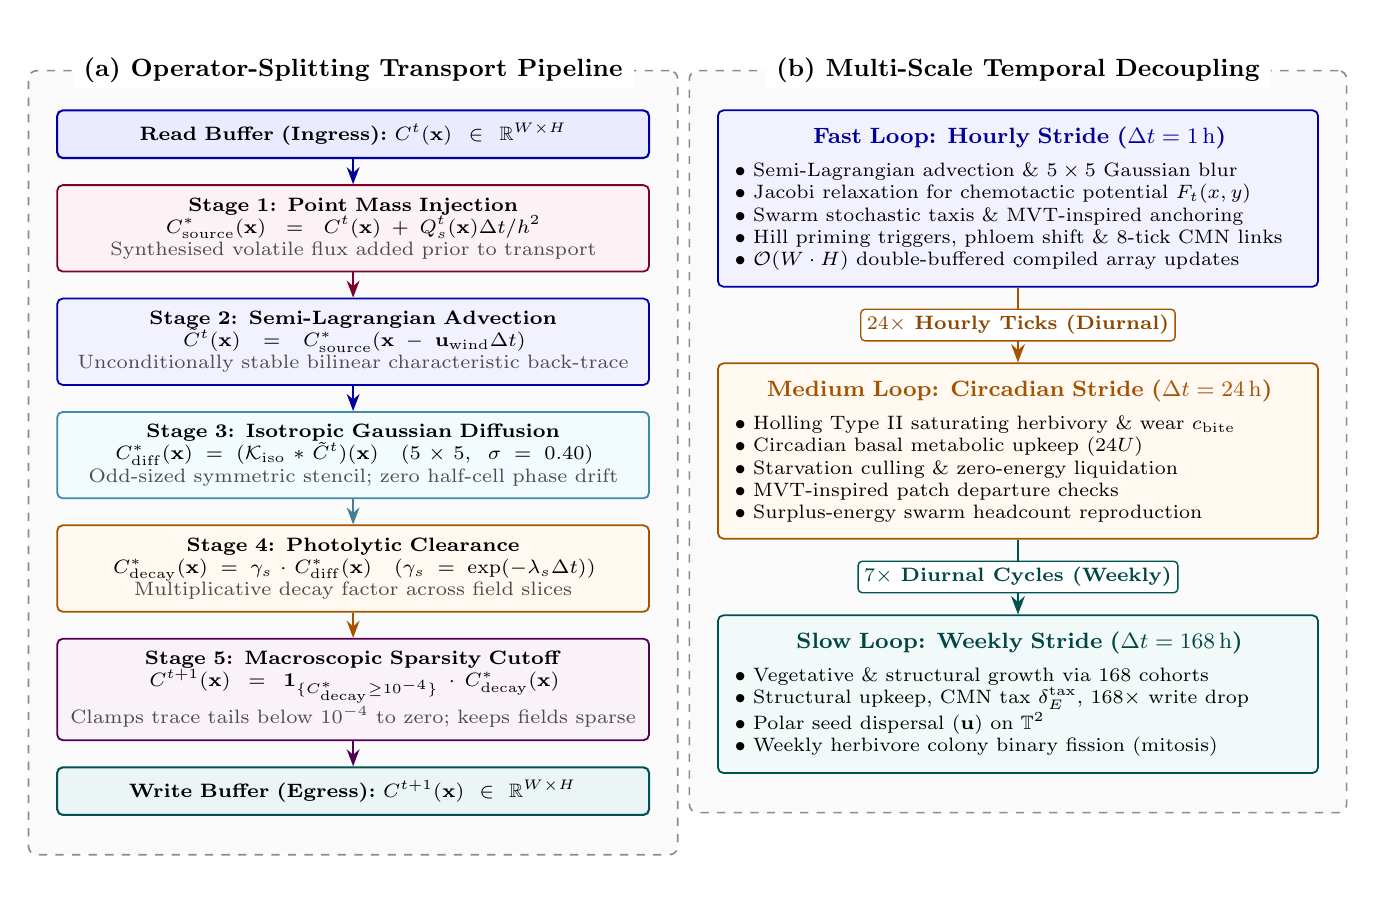
\begin{tikzpicture}[
    >=Stealth,
    font=\scriptsize,
    stage/.style={draw=#1!65!black, fill=#1!5, rounded corners=2pt, line width=0.65pt, inner sep=4.5pt, align=center, text width=7.2cm},
    buf/.style={draw=#1!65!black, fill=#1!8, rounded corners=2pt, line width=0.75pt, inner sep=4.5pt, align=center, text width=7.2cm},
    loopcard/.style={draw=#1!65!black, fill=#1!5, rounded corners=2pt, line width=0.65pt, inner sep=6pt, align=left, text width=7.2cm},
    panel/.style={draw=black!45, dashed, fill=black!2, rounded corners=3pt, line width=0.6pt, inner sep=10pt},
    badge/.style={draw=#1!65!black, fill=white, rounded corners=1.5pt, line width=0.5pt, inner sep=2.2pt, font=\scriptsize\bfseries, text=#1!55!black}
  ]

  % Panel (a): Relative vertical chain so zero box overlap
  \node[buf=blue] (r_buf) {\textbf{Read Buffer (Ingress):}\ $C^t(\mathbf{x}) \in \mathbb{R}^{W \times H}$};

  \node[stage=purple, below=0.32cm of r_buf] (s1) {%
    \textbf{Stage 1: Point Mass Injection}\\
    $C^{*}_{\mathrm{source}}(\mathbf{x}) = C^t(\mathbf{x}) + Q_s^t(\mathbf{x})\Delta t / h^2$\\
    {\scriptsize\color{black!70}Synthesised volatile flux added prior to transport}%
  };
  \node[stage=blue, below=0.32cm of s1] (s2) {%
    \textbf{Stage 2: Semi-Lagrangian Advection}\\
    $\tilde{C}^t(\mathbf{x}) = C^{*}_{\mathrm{source}}(\mathbf{x} - \mathbf{u}_{\mathrm{wind}}\Delta t)$\\
    {\scriptsize\color{black!70}Unconditionally stable bilinear characteristic back-trace}%
  };
  \node[stage=cyan, below=0.32cm of s2] (s3) {%
    \textbf{Stage 3: Isotropic Gaussian Diffusion}\\
    $C^{*}_{\mathrm{diff}}(\mathbf{x}) = (\mathcal{K}_{\mathrm{iso}} * \tilde{C}^t)(\mathbf{x}) \quad (5 \times 5,\; \sigma = 0.40)$\\
    {\scriptsize\color{black!70}Odd-sized symmetric stencil; zero half-cell phase drift}%
  };
  \node[stage=orange, below=0.32cm of s3] (s4) {%
    \textbf{Stage 4: Photolytic Clearance}\\
    $C^{*}_{\mathrm{decay}}(\mathbf{x}) = \gamma_s \cdot C^{*}_{\mathrm{diff}}(\mathbf{x}) \quad (\gamma_s = \exp(-\lambda_s\Delta t))$\\
    {\scriptsize\color{black!70}Multiplicative decay factor across field slices}%
  };
  \node[stage=violet, below=0.32cm of s4] (s5) {%
    \textbf{Stage 5: Macroscopic Sparsity Cutoff}\\
    $C^{t+1}(\mathbf{x}) = \mathbf{1}_{\{C^{*}_{\mathrm{decay}} \ge 10^{-4}\}} \cdot C^{*}_{\mathrm{decay}}(\mathbf{x})$\\
    {\scriptsize\color{black!70}Clamps trace tails below $10^{-4}$ to zero; keeps fields sparse}%
  };
  \node[buf=teal, below=0.32cm of s5] (w_buf) {\textbf{Write Buffer (Egress):}\ $C^{t+1}(\mathbf{x}) \in \mathbb{R}^{W \times H}$};

  \draw[->, line width=0.7pt, color=blue!60!black] (r_buf) -- (s1);
  \draw[->, line width=0.7pt, color=purple!65!black] (s1) -- (s2);
  \draw[->, line width=0.7pt, color=blue!60!black] (s2) -- (s3);
  \draw[->, line width=0.7pt, color=cyan!55!black] (s3) -- (s4);
  \draw[->, line width=0.7pt, color=orange!65!black] (s4) -- (s5);
  \draw[->, line width=0.7pt, color=violet!65!black] (s5) -- (w_buf);

  % Panel (b): Relative vertical chain with generous 0.95cm connector gap for badges
  \node[loopcard=blue, right=0.85cm of r_buf.north east, anchor=north west] (b1) {%
    \centering\textbf{\footnotesize\color{blue!60!black}Fast Loop: Hourly Stride ($\Delta t = 1\,\mathrm{h}$)}\\[4pt]
    \raggedright
    $\bullet$ Semi-Lagrangian advection \& $5\times 5$ Gaussian blur\\
    $\bullet$ Jacobi relaxation for chemotactic potential $F_t(x, y)$\\
    $\bullet$ Swarm stochastic taxis \& MVT-inspired anchoring\\
    $\bullet$ Hill priming triggers, phloem shift \& 8-tick CMN links\\
    $\bullet$ $\mathcal{O}(W\cdot H)$ double-buffered compiled array updates%
  };

  \node[loopcard=orange, below=0.95cm of b1] (b2) {%
    \centering\textbf{\footnotesize\color{orange!65!black}Medium Loop: Circadian Stride ($\Delta t = 24\,\mathrm{h}$)}\\[4pt]
    \raggedright
    $\bullet$ Holling Type~II saturating herbivory \& wear $c_{\mathrm{bite}}$\\
    $\bullet$ Circadian basal metabolic upkeep ($24 U$)\\
    $\bullet$ Starvation culling \& zero-energy liquidation\\
    $\bullet$ MVT-inspired patch departure checks\\
    $\bullet$ Surplus-energy swarm headcount reproduction%
  };

  \node[loopcard=teal, below=0.95cm of b2] (b3) {%
    \centering\textbf{\footnotesize\color{teal!55!black}Slow Loop: Weekly Stride ($\Delta t = 168\,\mathrm{h}$)}\\[4pt]
    \raggedright
    $\bullet$ Vegetative \& structural growth via $168$ cohorts\\
    $\bullet$ Structural upkeep, CMN tax $\delta_E^{\mathrm{tax}}$, $168\times$ write drop\\
    $\bullet$ Polar seed dispersal ($\mathbf{u}$) on $\mathbb{T}^2$\\
    $\bullet$ Weekly herbivore colony binary fission (mitosis)%
  };

  \draw[->, line width=0.8pt, color=orange!65!black] (b1.south) -- node[badge=orange] {$24\times$ Hourly Ticks (Diurnal)} (b2.north);
  \draw[->, line width=0.8pt, color=teal!65!black] (b2.south) -- node[badge=teal] {$7\times$ Diurnal Cycles (Weekly)} (b3.north);

  \begin{scope}[on background layer]
    \node[panel, fit=(r_buf)(w_buf), inner ysep=14pt] (pa) {};
    \node[panel, fit=(b1)(b3), inner ysep=14pt] (pb) {};
  \end{scope}

  \node[fill=white, anchor=center, font=\small\bfseries, inner xsep=4pt, inner ysep=2pt] (pa_lbl) at (pa.north) {(a) Operator-Splitting Transport Pipeline};
  \node[fill=white, anchor=center, font=\small\bfseries, inner xsep=4pt, inner ysep=2pt] (pb_lbl) at (pb.north) {(b) Multi-Scale Temporal Decoupling};

  % Explicit top/bottom padding so panel headers never clip
  \path ([yshift=0.30cm]pa_lbl.north) ([yshift=0.30cm]pb_lbl.north) ([yshift=-0.25cm]pa.south) ([yshift=-0.25cm]pb.south);
\end{tikzpicture}
}

  \caption{Operator-Splitting Numerical Scheme and Multi-Scale Temporal Decoupling Architecture. \textbf{(a)} Continuous airborne volatile transport is decomposed into a five-stage operator-splitting pipeline across double-buffered cellular tensors, coupling unconditionally stable semi-Lagrangian wind advection with isotropic Gaussian convolution and macroscopic sparsity clamping. \textbf{(b)} The multi-scale temporal hierarchy decouples execution across Fast ($1\,\text{h}$), Medium ($24\,\text{h}$), and Slow ($168\,\text{h}$) loops, resolving the rate disparity between hourly insect taxis and gradual vegetative growth while cutting per-tick plant-growth write traffic $168\times$ through phase-staggered cohort scheduling.}
  \label{fig:operator_splitting_pipeline}
\end{figure*}

To resolve plant--herbivore coevolutionary interactions with finite spatial lag and continuous chemical transport, PHIDS is formulated as a \textbf{coupled hybrid dynamical system}.

The simulation couples two operational layers: a discrete Lagrangian Entity--Component--System (ECS) governing mobile agent kinematics, somatic growth, and metabolic allocation, and a continuous Eulerian grid layer resolving parabolic reaction--diffusion--advection partial differential equations (PDEs), potential flow fields, and subterranean graph conduits. Below we formalise the global state space, continuous atmospheric transport, operator-splitting numerical integration, multi-scale temporal scheduling, and trophic kinetic laws.

% ------------------------------------------------------------------------------
\subsection{Global State Space and Domain Topology}
\label{subsec:state_space_topology}
% ------------------------------------------------------------------------------

The global ecosystem state at any discrete simulation epoch (tick) $t \in \mathbb{N}_0$ is represented by the unified state tuple:
\begin{equation}
  \mathcal{X}_t = \left( \mathcal{E}_t, \; \mathcal{G}_t, \; \mathcal{G}_{\text{myco}}, \; \mathcal{P} \right)
  \label{eq:global_state_tuple}
\end{equation}
where:
\begin{itemize}
  \item $\mathcal{E}_t = \{ e_1, e_2, \dots, e_{N(t)} \}$ denotes the discrete set of active biological entities instantiated within the Entity-Component-System (autotrophic flora anchors and mobile heterotrophic herbivore swarms), stored in contiguous Structure-of-Arrays (SoA) memory buffers.
  \item $\mathcal{G}_t \in \mathbb{R}^{W \times H \times K}$ represents the double-buffered Eulerian cellular field tensor over the spatial lattice $\Lambda$, tracking localised caloric densities, airborne volatile organic compound (VOC) concentrations across $K_{\text{voc}}$ channels, and defensive toxin layers across $K_{\text{tox}}$ channels.
  \item $\mathcal{G}_{\text{myco}} = (\mathcal{V}_{\text{flora}}, \mathcal{E}_{\text{hyphae}})$ defines the subterranean mycorrhizal fungal network, modelled as an unweighted, undirected nearest-neighbour lattice graph (cardinal adjacency) where vertices correspond to sessile root systems and edges represent active hyphal links.
  \item $\mathcal{P}$ represents the immutable global biophysical parameter set governing thermodynamic conversion efficiencies, kinetic rate constants, and environmental constants.
\end{itemize}

The spatial biotope spans a flat two-dimensional periodic domain $\Omega = [0, L_x) \times [0, L_y)$ ($\mathbb{T}^2$), discretised into an orthogonal cellular lattice $\Lambda = \{ (x, y) \in \mathbb{Z}^2 \mid 0 \le x < W, \; 0 \le y < H \}$ with uniform cell spacing $h = \Delta x = \Delta y$ and periodic toroidal wrapping across boundaries (accelerated via bitwise \texttt{AND} masking when $W, H$ are powers of two; Section~\ref{subsec:branchless_toroidal}). The discrete entity layer $\mathcal{E}_t$ advances synchronously with the Eulerian field layer $\mathcal{G}_t$ at fixed hourly ticks ($\Delta t = 1\,\text{h}$) without an asynchronous event queue: plants sample local volatile concentrations $C_s(x, y)$ against trigger thresholds and inject emissions $Q_s$ back into $\mathcal{G}_t$, while feeding, starvation culling, mitosis, somatic growth, and seed dispersal execute under deterministic diurnal ($24\,\text{h}$) and weekly ($168\,\text{h}$) strides.

% ------------------------------------------------------------------------------
\subsection{Continuous Atmospheric Transport Dynamics}
\label{subsec:atmospheric_transport}
% ------------------------------------------------------------------------------

Airborne communication between autotrophs relies on the atmospheric dispersion of volatile organic compounds (VOCs). Macroscopic transport of scalar substance $s \in \{1, \dots, K_{\text{voc}}\}$ across the periodic 2D domain is governed by the reaction-diffusion-advection Partial Differential Equation (PDE):
\begin{equation}
  \frac{\partial C_s}{\partial t} + \mathbf{u}_{\text{wind}} \cdot \nabla C_s = D_s \nabla^2 C_s - \lambda_s C_s + Q_s(\mathbf{x}, t),
  \label{eq:reaction_diffusion_pde}
\end{equation}
where $C_s(\mathbf{x}, t) \ge 0$ is local concentration, $\mathbf{u}_{\text{wind}} = (u_x, u_y)^{\top}$ in $\text{cells}\cdot\text{tick}^{-1}$ denotes the effective hourly plume-drift displacement rate capturing net canopy-trapped advection, sorption, and turbulent boundary-layer mixing rather than unattenuated meteorological velocity, $D_s > 0$ is the isotropic turbulent diffusivity, $\nabla^2 = \partial_x^2 + \partial_y^2$ is the planar Laplacian under periodic boundary conditions, $\lambda_s \ge 0$ is the photolytic clearance rate, and $Q_s(\mathbf{x}, t) = \sum_{i} q_{s,i}(t)\,\delta(\mathbf{x} - \mathbf{x}_i)$ aggregates active botanical emissions. Without clearance ($\lambda_s = 0$) and sources ($Q_s = 0$), periodic boundaries conserve total atmospheric mass identically.

% ------------------------------------------------------------------------------
\subsection{Operator Splitting and Numerical Scheme}
\label{subsec:operator_splitting}
% ------------------------------------------------------------------------------

Solving the coupled PDE~\eqref{eq:reaction_diffusion_pde} concurrently with tens of thousands of discrete kinematic agents over long time horizons requires an unconditionally stable numerical integration scheme. PHIDS employs a five-stage \textbf{operator-splitting method} (fractional step method), injecting active sources into the read buffer and decomposing continuous transport into discrete sequential operators:
\begin{equation}
  C_s^{t+1} = \left( \mathcal{S}_{\text{clamp}} \circ \mathcal{S}_{\text{decay}} \circ \mathcal{S}_{\text{diff}} \circ \mathcal{S}_{\text{adv}} \circ \mathcal{S}_{\text{source}} \right) \left( C_s^t \right)
  \label{eq:operator_splitting_pipeline}
\end{equation}
The mathematical formulation and algorithmic execution of each operator are defined as follows:

\paragraph{Stage 1: Localised Point Mass Injection ($\mathcal{S}_{\text{source}}$).}
Prior to atmospheric transport within the signalling step, botanical emissions synthesised by damaged host entities are added algebraically into the cellular lattice:
\begin{equation}
  C_{s,\text{source}}^t(x, y) = C_s^t(x, y) + \frac{Q_s^t(x, y) \Delta t}{h^2}
  \label{eq:mass_injection_step}
\end{equation}
where $Q_s^t(x, y)$ represents the aggregated volatile flux released by all active autotrophic emitters residing within cell $(x, y)$.

\paragraph{Stage 2: Semi-Lagrangian Advection ($\mathcal{S}_{\text{adv}}$).}
Traditional explicit finite-difference upwind schemes for hyperbolic advection are constrained by the Courant-Friedrichs-Lewy (CFL) stability criterion:
\begin{equation}
  \text{CFL} = \frac{\|\mathbf{u}_{\text{wind}}\|_{\infty} \Delta t}{h} \le 1.0
  \label{eq:cfl_condition}
\end{equation}
In high-velocity wind gusts, satisfying Equation~\eqref{eq:cfl_condition} requires sub-cycling the time step, increasing per-tick compute overhead. PHIDS bypasses the CFL ceiling through an unconditionally stable \textbf{semi-Lagrangian advection scheme} that traces incoming air parcels backwards to their upwind departure origin and interpolates concentration there.

For each lattice site $(x, y) \in \Lambda$, the algorithm traces the wind trajectory backwards in continuous time by displacement vector $\Delta \mathbf{x} = \mathbf{u}_{\text{wind}}(x, y) \Delta t$. The characteristic departure point is computed as:
\begin{align}
  x^* &= \text{wrap}\left( x - u_x(x, y) \Delta t, \; W \right) \label{eq:departure_point_x} \\
  y^* &= \text{wrap}\left( y - u_y(x, y) \Delta t, \; H \right) \label{eq:departure_point_y}
\end{align}
The advected scalar field $\tilde{C}_s^t(x, y)$ is evaluated via bilinear spatial interpolation across the four surrounding source-injected lattice anchors:
\begin{equation}
  \tilde{C}_s^t(x, y) = \sum_{i=0}^1 \sum_{j=0}^1 \omega_{ij} \, C_{s,\text{source}}^t\left( \lfloor x^* \rfloor + i, \; \lfloor y^* \rfloor + j \right)
  \label{eq:bilinear_interpolation}
\end{equation}
where the bilinear interpolation weights satisfy $\omega_{ij} \ge 0$ and $\sum_{i,j} \omega_{ij} = 1.0$. Because bilinear interpolation represents a convex combination of lattice values, the semi-Lagrangian operator is unconditionally $L^\infty$-stable:
\begin{equation}
  \|\tilde{C}_s^t\|_{\infty} \le \|C_{s,\text{source}}^t\|_{\infty} \quad \forall \; \Delta t > 0
  \label{eq:linfty_stability}
\end{equation}
completely eliminating numerical oscillations or explosive divergence regardless of wind velocity. Because bilinear backward interpolation forms a Bernoulli convex combination across adjacent lattice nodes along each axis with fractional Courant displacement $\alpha \in [0, 1)$, it introduces implicit numerical diffusion with per-step variance $\sigma_{\text{num}}^2(\alpha) = \alpha(1 - \alpha)$ \cite{staniforth1991semi}. This implicit diffusivity vanishes at integer displacements ($\alpha = 0$) and peaks at $\sigma_{\text{num}}^2(0.5) = 0.25$ for $\|\mathbf{u}_{\text{wind}}\| = 0.50\,\text{cells/tick}$ --- $56\%$ larger than the explicit Gaussian kernel variance $\sigma^2 = 0.16$ in Stage~3 --- creating slight additional lateral smoothing at half-cell Courant displacements.

\paragraph{Stage 3: Isotropic Gaussian Diffusion ($\mathcal{S}_{\text{diff}}$).}
Following advective displacement, spatial diffusion is resolved via discrete two-dimensional spatial convolution using a uniform diffusivity kernel shared across channels ($D_s \equiv D$), evaluated over a symmetric, odd-sized isotropic Gaussian stencil $\mathcal{K}_{\text{iso}} \in \mathbb{R}^{5 \times 5}$:
\begin{align}
  C_{s,\text{diff}}^{*}(x, y) &= \left( \mathcal{K}_{\text{iso}} * \tilde{C}_s^t \right)(x, y) \nonumber \\
  &= \sum_{u=-2}^2 \sum_{v=-2}^2 \mathcal{K}_{\text{iso}}[u, v] \, \tilde{C}_s^t(x - u, y - v)
  \label{eq:gaussian_convolution}
\end{align}
The discrete stencil $\mathcal{K}_{\text{iso}}[u, v] = w_{u,v} / \sum_{i,j=-2}^{2} w_{i,j}$ normalises bivariate Gaussian weights $w_{u,v} = \exp\!\left(-(u^2 + v^2) / (2\sigma^2)\right)$ over the odd-sized $5 \times 5$ window ($u, v \in \{-2, \dots, 2\}$) with default $\sigma = 0.40$. Centring an odd-sized stencil on $(0, 0)$ eliminates the half-cell diagonal phase drift ($+0.5h, +0.5h$) inherent to even-sized kernels while unit normalisation ($\sum_{u,v}\mathcal{K}_{\text{iso}}[u,v]=1.0$) preserves volatile mass; at $\sigma = 0.40$, outer weights beyond radius $2$ fall below $\epsilon_{\text{signal}} = 10^{-4}$ (yielding compact $3 \times 3$ effective dispersion while retaining $5 \times 5$ stencil support for broader diffusivities).

\paragraph{Stage 4: Photolytic Chemical Clearance ($\mathcal{S}_{\text{decay}}$).}
Atmospheric degradation is integrated via the first-order exponential decay operator:
\begin{align}
  C_{s,\text{decay}}^{*}(x, y) &= \gamma_s \cdot C_{s,\text{diff}}^{*}(x, y) \nonumber \\
  \text{where } \gamma_s &= \exp\left( -\lambda_s \Delta t \right) \approx 1 - \lambda_s \Delta t
  \label{eq:photolytic_decay_step}
\end{align}
The linear approximation $\gamma_s = 1 - \lambda_s \Delta t$ is accurate to first order in $\lambda_s \Delta t$ (with $\mathcal{O}((\lambda_s \Delta t)^2)$ truncation error) when $\lambda_s \Delta t \ll 1$; the compiled solver evaluates this multiplicative retention factor directly across vectorised registers.

\paragraph{Stage 5: Macroscopic Sparsity Cutoff ($\mathcal{S}_{\text{clamp}}$).}
Under multiplicative clearance ($\gamma_s < 1$), exponential decay tails persist indefinitely across the periodic torus at negligible amplitude, causing unphysical background accumulation over thousands of ticks and preventing fast sparse checks ($\max C_s < \epsilon_{\text{signal}}$). To enforce finite-horizon plume extinction and maintain sparse active signal sets in double-precision field buffers, PHIDS applies a branchless threshold mask against $\epsilon_{\text{signal}} = 1.0 \times 10^{-4}$:
\begin{equation}
  C_s^{t+1}(x, y) = \mathbf{1}_{\{ C_{s,\text{decay}}^{*}(x, y) \ge \epsilon_{\text{signal}} \}} \cdot C_{s,\text{decay}}^{*}(x, y),
  \label{eq:subnormal_clamping}
\end{equation}
clamping sub-threshold residues directly to exact floating-point zero.

The sequential composition in Equation~\eqref{eq:operator_splitting_pipeline} constitutes a first-order Lie-Trotter operator splitting scheme. Let $\mathcal{A} = -\mathbf{u} \cdot \nabla$ and $\mathcal{B} = D \nabla^2 - \lambda$; applying $\mathcal{A}$ prior to $\mathcal{B}$ corresponds to the composition $\exp(\mathcal{B}\Delta t)\exp(\mathcal{A}\Delta t)$. By the Baker-Campbell-Hausdorff (BCH) formula:
\begin{align}
  \exp\left( (\mathcal{A} + \mathcal{B})\Delta t \right) &= \exp(\mathcal{B}\Delta t) \exp(\mathcal{A}\Delta t) \nonumber \\
  &\quad + \frac{\Delta t^2}{2} [\mathcal{A}, \mathcal{B}] + \mathcal{O}(\Delta t^3)
  \label{eq:bch_splitting_error}
\end{align}
where $[\mathcal{A}, \mathcal{B}] = \mathcal{A}\mathcal{B} - \mathcal{B}\mathcal{A}$ is the Lie commutator bracket. Because advection and diffusion do not commute in general non-uniform wind fields ($[\mathcal{A}, \mathcal{B}] \neq 0$), splitting introduces a local truncation error of $\mathcal{O}(\Delta t^2)$ and a global error of $\mathcal{O}(\Delta t)$ (vanishing when $\mathbf{u}_{\text{wind}}$ is spatially uniform as in the orchard reference runs, since constant-coefficient advection and Laplacian diffusion commute).

% ------------------------------------------------------------------------------
\subsection{Chemotactic Potential and Jacobi Relaxation}
\label{subsec:chemotactic_potential}
% ------------------------------------------------------------------------------

Herbivore swarms navigate heterogeneous biotopes through chemotaxis -- orienting along spatial gradients of chemical attractants and repellents. To avoid computing individual $A^*$ or Dijkstra shortest paths for thousands of swarms ($\mathcal{O}(N_{\text{swarms}} \cdot W H \log(WH))$), PHIDS constructs a single \textbf{unified chemotactic flow field} $F_t(x, y)$ per tick, which all agents query locally in $\mathcal{O}(1)$ time. At the start of each hourly tick, an un-diffused baseline desirability surface $G_t(x, y)$ is constructed by weighting local plant energy with foliar apparent nutrition $\eta(x, y)$ and subtracting accumulated toxins:
\begin{equation}
  G_t(x, y) = \alpha \, E_{\text{plant}}(x, y) \, \eta(x, y) - \beta \sum_{k=1}^{K_{\text{tox}}} T_{k,t}(x, y)
  \label{eq:baseline_gradient}
\end{equation}
where $E_{\text{plant}}(x, y)$ is the host plant energy at coordinate $(x, y)$ (zero on unoccupied cells), $\eta(x, y) \in [\eta_{\min}, 1.0]$ is the local vascular palatability multiplier, $T_{k,t}(x, y)$ is the concentration of the $k$-th defensive toxin channel, and $\alpha > 0$, $\beta > 0$ are attraction and aversion coupling weights. Linear summation over toxin channels $\sum_k T_k$ enforces sensory non-masking so overlapping chemical defences build repulsive barriers.

To turn point sources into a long-range sensory surface detectable across empty space, $G_t(x, y)$ undergoes iterative diffusion via Jacobi relaxation. On lattice spacing $h = 1$, the continuous screened Poisson counterpart with screening constant $\kappa$ reads:
\begin{equation}
  \nabla^2 F(\mathbf{x}) - \kappa^2 F(\mathbf{x}) = -\frac{4}{\delta h^2} G_t(\mathbf{x}),
  \label{eq:screened_poisson}
\end{equation}
whose 4-point central-difference steady-state fixed point $(1-\delta) F - \frac{\delta}{4}\Delta_5 F = G_t$ with spatial decay factor $\delta \in (0, 1)$ yields the iterative Jacobi update rule implemented in the engine:
\begin{align}
  F^{(m+1)}[x, y] &= G_t[x, y] + \frac{\delta}{4} \Big( F^{(m)}[x+1, y] \nonumber \\
  &\quad + F^{(m)}[x-1, y] + F^{(m)}[x, y+1] \nonumber \\
  &\quad + F^{(m)}[x, y-1] \Big)
  \label{eq:jacobi_iteration_rule}
\end{align}
where $\kappa^2 = \frac{4(1-\delta)}{\delta h^2}$ links the discrete decay factor $\delta$ to continuous screening, iterates initialise directly from the baseline surface ($F^{(0)} = G_t$), coordinate offsets use periodic toroidal wrapping, and sweeps stop at $M_{\max} = W + H$ iterations (switching automatically to OpenMP parallel kernels when $W \cdot H \ge 128^2$). The iteration terminates when the maximum absolute grid residual falls below the convergence tolerance $\epsilon_{\text{jacobi}}$ or when the maximum iteration limit $M_{\max}$ is reached:
\begin{align}
  \max_{(x, y) \in \Lambda} \left| F^{(m+1)}[x, y] - F^{(m)}[x, y] \right| &< \epsilon_{\text{jacobi}} = 10^{-4} \nonumber \\
  &\quad \text{or } m \ge M_{\max}
  \label{eq:jacobi_stopping_criterion}
\end{align}
Equation~\eqref{eq:jacobi_iteration_rule} is compiled into multithreaded native machine code for large lattices ($W \cdot H \ge 128^2$) and serial compiled loops on smaller grids. After relaxation converges, host camouflage attenuates local surface attractiveness in-place via $F_t(x, y) \gets \Phi_{\text{camo}}(x, y)\,F_t(x, y)$ ($\Phi_{\text{camo}} \in [0, 1]$), hiding masked flora from nearby foragers. Because each update for cell $(x, y)$ depends strictly on the read buffer $F^{(m)}$ and writes exclusively to $F^{(m+1)}$, inner loops execute with zero write-after-read hazards.

% ------------------------------------------------------------------------------
\subsection{Swarm Kinematics and Stochastic Taxis}
\label{subsec:swarm_kinematics}
% ------------------------------------------------------------------------------

Heterotrophic herbivore swarms navigate the relaxed potential field $F_t(x, y)$ through local sampling. Sensory perception in biological foragers is noisy rather than deterministic gradient ascent ($\arg\max F$), which would produce artificial single-file trajectories. A swarm with integer movement period $v_i \in \mathbb{N}^+$ moves whenever its movement cooldown ($v_i - 1\,\text{ticks}$ after each step) reaches zero, corresponding to step cadence $1/v_i \in (0, 1]\,\text{cells/h}$, sampling $F_t$ over its 5-cell \textbf{von Neumann neighbourhood}:
\begin{align}
  \mathcal{V}(x, y) = \big\{ &(x, y), \; (x+1, y), \; (x-1, y), \nonumber \\
  &(x, y+1), \; (x, y-1) \big\}
  \label{eq:von_neumann_neighborhood}
\end{align}
where spatial indices wrap toroidally. Restricting candidate moves to orthogonal nearest neighbours enforces an exact $1:1$ grid step ($h$) without diagonal $\sqrt{2}h$ step-length distortion. Scalar potential differences map to transition probabilities via \textbf{Boltzmann softmax action selection}:
\begin{equation}
  P(u, v \mid x, y) = \frac{\exp\left( \frac{F_t(u, v) - F_{\max}}{\tau} \right)}{\sum_{(u', v') \in \mathcal{V}(x, y)} \exp\left( \frac{F_t(u', v') - F_{\max}}{\tau} \right)}
  \label{eq:boltzmann_softmax}
\end{equation}
where $F_{\max} = \max_{(u, v) \in \mathcal{V}} F_t(u, v)$ prevents exponential overflow and $\tau > 0$ sets sensory temperature (in the engine's alternative $\tau = 0$ linear-weighted mode, weights equal $F_t(u, v) - F_{\min}$). Calibrating $\tau \in [0.15, 0.40]$ balances chemotactic gradient ascent ($\tau \to 0^+$) against exploratory dispersal ($\tau \to \infty$, $P = 0.20$).

Across depleted terrain where chemical gradients vanish ($\max F_t - \min F_t < 1.0 \times 10^{-6}$), swarms preserve their movement heading through \textbf{orthokinetic persistence}: letting $\mathbf{d}_t = (dx_t, dy_t)$ denote the previous step vector, candidate weights are biased forward by $W_{\text{ortho}} = 10.0$:
\begin{equation}
  w(u, v) = \begin{cases}
    W_{\text{ortho}}, & \text{if } (u - x, v - y) = (dx_t, dy_t) \\
    1.0, & \text{otherwise}
  \end{cases}
  \label{eq:orthokinetic_weight}
\end{equation}
giving $P_{\text{forward}} = 10/14 \approx 0.714$ and turning probability $0.071$ per orthogonal/reverse edge. Once situated on a host, patch departure uses a strictly local $\mathcal{O}(1)$ MVT-inspired logistic heuristic based on the intake-to-upkeep ratio $\mathcal{R}_{\text{intake}} = \Delta E_{\text{consumed}} / E_{\text{upkeep}}$ (rather than solving a global MVT habitat optimisation):
\begin{equation}
  P_{\text{depart}} = \frac{1}{1 + \exp\left( k_{\text{mvt}} \left( \mathcal{R}_{\text{intake}} - 1.0 \right) \right)}
  \label{eq:mvt_logistic_departure}
\end{equation}
with steepness $k_{\text{mvt}} = 5.0$, keeping swarms anchored while feeding is plentiful ($\mathcal{R}_{\text{intake}} \gg 1$) and driving departure once reserves drop ($P_{\text{depart}} \approx 0.993$ as $\mathcal{R}_{\text{intake}} \to 0$). Finally, movement prevents overcrowding via a branchless tile carrying-capacity mask zeroed prior to sampling:
\begin{equation}
  M_{\text{cap}}(u, v) = \mathbf{1}_{\left\{ N_{\text{pop}}(u, v) < C_{\max} \right\}},
  \label{eq:capacity_mask}
\end{equation}
compelling surplus agents to divert to adjacent spatial refugia.

% ------------------------------------------------------------------------------
\subsection{Multi-Scale Temporal Decoupling}
\label{subsec:temporal_decoupling}
% ------------------------------------------------------------------------------

Ecological systems operate across vastly divergent temporal scales. Herbivore taxis and atmospheric plume dispersion occur on the order of seconds to hours ($\Delta \tau \approx 1\,\text{h}$), whereas circadian feeding and digestive cycles operate on a diurnal cadence ($24\,\text{h}$), and autotrophic vegetative growth, seed germination, and mycorrhizal development require weeks ($168\,\text{h}$).

In classical simulation architectures, integrating all biological rates at hourly resolution ($\Delta t = 1\,\text{h}$) forces slow-growing species parameterised with low hourly growth percentages $g$ (e.g. $g = 0.05\%\,\text{h}^{-1}$) to apply small per-tick increments:
\begin{align}
  \Delta E_{\text{hourly}} &= E_{\text{base}} \cdot \frac{g}{100} \nonumber \\
  &\approx 100 \cdot 0.0005 = 0.05\,\text{cal}\,\text{h}^{-1}
  \label{eq:microscopic_increment}
\end{align}
where $E_{\text{base}} = 100\,\text{cal}$ denotes a nominal vegetative reserve and $g$ is the species-specific hourly growth percentage (high-turnover orchard benchmarks use elevated $g = 4.5\%\,\text{h}^{-1}$, whereas slow forest flora exhibit small hourly fractions). Although double-precision (\texttt{float64}) energy arrays add $\Delta E_{\text{hourly}}$ to mature reserves ($E_{\text{plant}} \sim 10^3\,\text{cal}$) without precision loss, scanning and mutating thousands of dormant plant entities every hourly tick wastes memory bandwidth and evicts active field slices from L1/L3 caches.

To avoid redundant per-tick writes while preventing macro-telemetry sawtooth shocks, PHIDS uses a \textbf{multi-scale temporal decoupling hierarchy} partitioned across three nested clock cycles alongside a configurable root-link interval:
\begin{enumerate}
  \item \textbf{Fast Loop ($\Delta t = 1\,\text{h}$, every tick):} Evaluates Jacobi potential relaxation, camouflage attenuation, MVT-inspired host anchoring checks, Boltzmann softmax swarm taxis, Hill defence triggers, toxin lethality and eviction walks, aftereffect timers, vascular phloem translocation and recovery ($\eta(t)$), semi-Lagrangian advection, Gaussian diffusion, and photolytic clearance.
  \item \textbf{Symbiotic Graph Interval ($\Delta t = 8\,\text{h}$, configurable):} Evaluates dynamic mycorrhizal cardinal root-link establishment ($8$-tick default interval) and prunes links attached to culled hosts.
  \item \textbf{Medium Loop ($\Delta t = 24\,\text{h}$, diurnal stride):} Evaluates Holling Type~II herbivory on stationary non-repelled swarms, diurnal metabolic upkeep ($24 U$), starvation culling, and surplus-energy swarm reproduction.
  \item \textbf{Slow Loop ($\Delta t = 168\,\text{h}$, weekly stride):} Executes phase-staggered plant cohort growth, structural tissue accretion and maintenance, weekly CMN link upkeep, and seed dispersal (gated per species by reproduction intervals $868\text{--}1{,}737\,\text{ticks}$), alongside weekly swarm binary fission.
\end{enumerate}

To avoid synchronous execution shocks where all plants update simultaneously on tick $t = 168, 336, \dots$ (causing periodic frame-time spikes), the autotrophic population is partitioned into $168$ disjoint \textbf{phase-staggered cohorts}. Let $\Delta E_{\mathrm{wk}} = 168\,\Delta E_{\text{hourly}}$. Entity $e_i$ executes its weekly update solely on cohort ticks $i \equiv t \pmod{168}$, remaining read-only otherwise:
\begin{equation}
  E_{i}^{t+1} =
  \begin{cases}
    \min(E_i^t + \Delta E_{\mathrm{wk}},\, E_{\max}), & i \equiv t \pmod{168}, \\
    E_i^t, & \text{otherwise}.
  \end{cases}
  \label{eq:full_weekly_growth}
\end{equation}
This cohort stride distributes the computational workload evenly across all $168$ ticks of the week, reducing per-tick plant-growth memory writes by a factor of $168$ while preserving macroscopic weekly continuity and cache locality.

% ------------------------------------------------------------------------------
\subsection{Multi-Trophic Kinetics and Defence Stoichiometry}
\label{subsec:trophic_kinetics}
% ------------------------------------------------------------------------------

On each weekly cohort tick ($i \equiv t \pmod{168}$), plants with positive structural ceiling $M_{\max, j} > 0$ also accrue permanent structural tissue mass and pay cohort-scaled structural upkeep together with weekly mycorrhizal link maintenance:
\begin{align}
  M_j^{t+168} &= \min\!\left(M_{\max, j},\; M_j^t + 168\,g_{\text{struct}, j}\right), \nonumber \\
  \Delta E_{\text{struct}, j} &= 0.5\,E_{\min, j}\,\frac{M_j^{t+168}}{M_{\max, j}}, \nonumber \\
  \Delta E_{\text{myco}, j} &= \delta_E^{\text{tax}} \cdot \deg_{\mathcal{G}_{\text{myco}}}(e_j),
  \label{eq:structural_mass_growth}
\end{align}
deducted from $E_j$ prior to survival culling at $E_j < E_{\min, j}$ (with dead hosts removed and incident edges pruned from $\mathcal{G}_{\text{myco}}$). Every $8$ ticks (or if equal to a weekly boundary), disjoint adjacent plant pairs $(e_j, e_k)$ at Manhattan distance $1$ satisfying $E - c_{\text{conn}} \ge E_{\min}$ establish an undirected edge in $\mathcal{G}_{\text{myco}}$ at symmetrical carbon expenditure $E_j \gets E_j - c_{\text{conn}}$, $E_k \gets E_k - c_{\text{conn}}$.

On diurnal feeding ticks ($t \bmod 24 = 0$), stationary, non-repelled swarms extract biomass from a co-located compatible host $e_j$ via the \textbf{Holling Type~II functional response}~\cite{holling1959components} scaled by step cadence $1/\max(1, v_i)$:
\begin{align}
  a_{\text{eff}, i} &= \frac{a_i}{\max(1, v_i)}, \nonumber \\
  \Delta E_{i \leftarrow j} &= \min\!\left(E_j,\; \frac{a_{\text{eff}, i}\, E_j}{1 + a_{\text{eff}, i}\, T_h^{\text{stride}}\, E_j} \cdot N_i\right),
  \label{eq:math_holling_type_ii}
\end{align}
where $a_i$ ($\mathrm{stride}^{-1}$) and $T_h^{\text{stride}}$ ($\mathrm{stride}\cdot\mathrm{cal}^{-1}$) act at unit diurnal stride multiplier ($\Delta_{\text{stride}} = 1.0$, setting the per-event intake ceiling at $1/T_h^{\text{stride}}$ calories per individual), $N_i$ is swarm headcount, and dividing by movement period $\max(1, v_i)$ reduces effective attack rate monotonically as step cadence $1/v_i$ slows; in the worst-case hourly regime of Proposition~\ref{thm:critical_synthesis_delay}, $v_i = 1$ and Eq.~\eqref{eq:math_holling_type_ii} acts every hour. Assimilated energy increments swarm reserve by $e_{\text{eff}}(1 - \delta_{\mathrm{morph}, j})\Delta E_{i \leftarrow j}$. In parallel, constitutive mechanical wear inflicts stochastic per-bite casualties governed by damage parameter $c_{\mathrm{bite},j} \ge 0$ and morphological adaptation $\alpha_{\mathrm{morph},i} \in [0, 1]$:
\begin{align}
  d_{ij} &= c_{\mathrm{bite},j}\,(1 - \alpha_{\mathrm{morph},i}), \nonumber \\
  \Delta N_{\text{mech}} &= \lfloor d_{ij} \rfloor + \operatorname{Bernoulli}\!\left(d_{ij} - \lfloor d_{ij} \rfloor\right).
  \label{eq:mechanical_wear}
\end{align}

Diurnally (unless temporarily evicted by a repellent toxin), active swarms deduct $24$-hour metabolic respiration $\Delta E_{\text{upkeep}, i} = 24\,N_i\,E_{\min, i}\,U_i$. Surplus energy above baseline maintenance $N_i E_{\min, i}$ funds net-assimilation headcount reproduction, while oversized swarms split symmetrically via binary fission on weekly Slow Loop boundaries ($t \bmod 168 = 0$ when $N_i \ge N_{\text{split}, i}$):
\begin{align}
  \Delta N_{\text{birth}, i} &= \left\lfloor \frac{\max\!\left(0,\, E_i - N_i E_{\min, i}\right)}{\max\!\left(E_{\min, i},\, d_{\text{rep}, i} E_{\min, i}\right)} \right\rfloor, \nonumber \\
  N_{\text{child}} &= \left\lfloor \frac{N_i}{2} \right\rfloor, \qquad E_{\text{child}} = \frac{E_i}{2},
  \label{eq:swarm_repro_mitosis}
\end{align}
placing the daughter swarm onto an adjacent von Neumann cell.

Neighbouring flora sense airborne VOC concentrations through non-linear cooperative binding via the \textbf{Hill function}:
\begin{equation}
  S(C_{\text{voc}}) = \frac{C_{\text{voc}}^n}{K_d^n + C_{\text{voc}}^n},
  \label{eq:hill_priming_function}
\end{equation}
where $n \in [2, 4]$ denotes cooperativity, $K_d$ is the half-saturation threshold, and $C_{\text{voc}}$ is local signal concentration. Exceeding $S(C_{\text{voc}}) \ge \tau_{\text{prim}}$ activates downstream priming triggers, compressing inducible synthesis delay from $\theta_{\text{synth}}$ to $\theta_{\text{primed}} \ll \theta_{\text{synth}}$. While its activation trigger remains true, an active chemical substance refreshes its persistence window to $\tau_{\text{aft}}$ ticks; once the trigger clears, reversible synthesis remains active and decrements $\tau_{\text{aft}}$ by $1$ per tick until deactivation at zero (or aborts immediately if maintenance cost $c_{\text{synth}}$ would drive host energy below $E_{\min, j}$). When an active toxin channel $T_s(x, y) \le 1.0$ contacts a co-located swarm with lethality rate $\mu_{\text{tox}, s} \ge 0$, casualties and repellent eviction follow:
\begin{align}
  \Delta N_{\text{tox}} &= \left\lfloor \mu_{\text{tox}, s}\,T_s(x, y)\,N_i \right\rfloor, \nonumber \\
  E_i &\gets \max\!\left(0,\, E_i - \Delta N_{\text{tox}}\,E_{\min, i}\right), \nonumber \\
  t_{\text{rep}, i} &\gets \tau_{\text{walk}, s},
  \label{eq:toxin_casualties_repulsion}
\end{align}
where lethal losses decrement $N_i \gets \max(0, N_i - \Delta N_{\text{tox}})$ and non-repelled swarms entering a repellent barrier ($\tau_{\text{walk}, s} > 0$) execute an undirected 5-cell von Neumann random walk for $\tau_{\text{walk}, s}$ ticks while diurnal metabolism and reproduction pause.

When an injured host emits warning signal flux $S_{\text{emit}}$, the engine partitions the budget between the airborne field and subterranean cardinal neighbours in $\mathcal{G}_{\text{myco}}$ ($N_{\text{relay}} = \deg_{\mathcal{G}_{\text{myco}}}(e_j)$):
\begin{align}
  S_{\text{airborne}} &= \frac{S_{\text{emit}}}{N_{\text{relay}} + 1}, \label{eq:myco_airborne} \\
  S_{\text{relay,total}} &= S_{\text{emit}} \cdot \frac{N_{\text{relay}}}{N_{\text{relay}} + 1}. \label{eq:myco_subterranean}
\end{align}
Each connected neighbour $k \in \{1, \dots, N_{\text{relay}}\}$ receives an unattenuated direct increment scaled by the dimensionless hyphal relay gain $g_{\text{relay}} \ge 1$:
\begin{equation}
  \Delta S_{\text{relay}, k} = \left( \frac{S_{\text{emit}}}{N_{\text{relay}} + 1} \right) \cdot g_{\text{relay}}.
  \label{eq:myco_neighbor_flux}
\end{equation}
Strict mass conservation holds at $g_{\text{relay}} = 1$, whereas $g_{\text{relay}} > 1$ applies an amplified relay multiplier at weekly per-link carbon upkeep $\delta_E^{\text{tax}}$. Every tick during the signalling phase, vascular phloem withdrawal adjusts apparent foliar nutrition $\eta(t) \in [\eta_{\min}, 1.0]$ toward $\eta_{\text{target}}$ via $\eta(t+1) = \eta(t) + (\eta_{\text{target}} - \eta(t))\,\gamma_{\text{translocation}}$; once withdrawal expires, palatability recovers monotonically via:
\begin{equation}
  \eta(t+1) = \eta(t) + \left( 1.0 - \eta(t) \right) \cdot \gamma_{\text{translocation}},
  \label{eq:phloem_recovery_recurrence}
\end{equation}
with translocation rate $\gamma_{\text{translocation}} \in (0, 1)$.

Plant reproduction uses an $\mathcal{O}(1)$ \textbf{stochastic polar ray-casting kernel} motivated by Okubo and Levin~\cite{okubo2001diffusion}: sampling $d \sim U(d_{\min}, d_{\max})$, computing normalised wind vector $\mathbf{u} = \mathbf{u}_{\text{wind}} / \|\mathbf{u}_{\text{wind}}\|$ (or isotropic $\theta \sim U(0, 2\pi)$ under calm wind $\|\mathbf{u}_{\text{wind}}\| \le 10^{-9}$), drawing lateral dispersion $\delta_\perp \sim \mathcal{N}(0, \sigma_\perp^2)$ with $\sigma_\perp = \max(0.15, 0.35 d)$, and placing seedlings at:
\begin{align}
  x_{\text{target}} &= \text{round}\left( x_0 + d u_x - \delta_\perp u_y \right), \label{eq:seed_projection_x} \\
  y_{\text{target}} &= \text{round}\left( y_0 + d u_y + \delta_\perp u_x \right), \label{eq:seed_projection_y}
\end{align}
deducting $E_{\text{seed}}$ from the parent and initialising unoccupied seedlings at $E_{\text{base}}$ and $M_j = 0$; whenever a parameterisation sets $E_{\text{base}} > E_{\text{seed}}$, the difference $E_{\text{base}} - E_{\text{seed}}$ represents an explicit establishment-carbon subsidy from seedbank or early cotyledon reserves (Proposition~\ref{prop:capacity_boundedness}). Conversely, whenever a swarm's energy $E_i$ drops below zero during diurnal upkeep, integer casualties are cleared immediately and remaining fractional debt is discarded:
\begin{align}
  \Delta N_{\text{starve}} &= \left\lceil \frac{-E_i}{E_{\text{min}}} \right\rceil, \nonumber \\
  N_i &\gets \max\!\left(0,\, N_i - \Delta N_{\text{starve}}\right), \qquad E_i \gets 0.0,
  \label{eq:integer_casualty_clearing}
\end{align}
preventing ghost metabolic debt and unregistering empty swarms.

% ------------------------------------------------------------------------------
\subsection{Global Deterministic System Composition}
\label{subsec:system_composition}
% ------------------------------------------------------------------------------

The temporal advancement of the entire coupled ecosystem from epoch $t$ to $t+1$ is formalised by the ordered composition of phase operators:
\begin{align}
  \mathcal{X}_{t+1} = \big( &\mathcal{T}_{\text{term}} \circ \mathcal{T}_{\text{telem}} \circ \mathcal{T}_{\text{rebuild}} \circ \mathcal{T}_{\text{signal}} \nonumber \\
  &\circ \mathcal{T}_{\text{interact}} \circ \mathcal{T}_{\text{life}} \circ \mathcal{T}_{\text{flow}} \big) \left( \mathcal{X}_t \right)
  \label{eq:phase_operator_chain}
\end{align}
The causal precedence of this sequence is strictly non-commutative:
\begin{enumerate}
  \item $\mathcal{T}_{\text{flow}}$: Solves the Jacobi potential equation over $\mathcal{G}_t$ and applies autotrophic camouflage attenuation to construct the unified chemotactic field $F_t(x, y)$.
  \item $\mathcal{T}_{\text{life}}$: Integrates phase-staggered autotrophic caloric and structural growth, structural maintenance, weekly mycorrhizal link tax, 8-tick CMN growth, and stochastic seed dispersal.
  \item $\mathcal{T}_{\text{interact}}$: Executes Boltzmann softmax swarm taxis, resolves diurnal Holling Type~II grazing extractions, applies mechanical damage, and enforces integer starvation culling and weekly binary swarm mitosis.
  \item $\mathcal{T}_{\text{signal}}$: Evaluates defence triggers, updates phloem nutrition withdrawal/recovery, injects botanical volatile and mycorrhizal emissions $Q_s$, applies toxin lethality and repulsion, decrements aftereffect windows, and advances the five-stage PDE operator-splitting scheme.
  \item $\mathcal{T}_{\text{rebuild}}$: Recomputes aggregate plant energy and structural mass layers from per-species write buffers and commits double-buffered array swaps.
  \item $\mathcal{T}_{\text{telem}}$: Serialises component metrics and field tensors into chunked replay buffers.
  \item $\mathcal{T}_{\text{term}}$: Evaluates macroscopic stopping criteria (e.g. total biotope defoliation or herbivore extinction).
\end{enumerate}

By partitioning lattice field updates between read-only source buffers and pre-allocated write buffers, Equation~\eqref{eq:phase_operator_chain} supports deterministic thread-count-invariant execution under upfront PRNG seeding (Section~\ref{subsec:double_buffering_zarr}).


% ==============================================================================
% Section 5: Analytical Properties, Bounds & Formal Proofs
% ==============================================================================
% ==============================================================================
% Section 5: Analytical Properties and System Bounds
% ==============================================================================

\section{Analytical Properties and System Bounds}
\label{sec:theoretical_invariants}

Hybrid models that couple discrete agent states with continuous reaction-diffusion-advection partial differential equations (PDEs) require explicit energy-accounting bounds and dynamical consistency conditions. Unconstrained agent update rules can violate carrying-capacity bounds or obscure the timescale separation between grazing depletion and biochemical induction. This section establishes three analytical properties of the model: bounded capacity and non-reproductive metabolic dissipation (Proposition~\ref{prop:capacity_boundedness}), the worst-case continuous-grazing critical synthesis delay $\theta_{\mathrm{crit}}$ (Proposition~\ref{thm:critical_synthesis_delay}), and the mean-field delay-bifurcation threshold $\tau^*$ (Proposition~\ref{thm:hopf_limit_cycle}). Double-buffered memory isolation and cross-thread reproducibility belong to the software implementation and are presented in Section~\ref{subsec:double_buffering_zarr}.

\begin{figure*}[t]
  \centering
  % ==============================================================================
% Figure 6: Analytical Invariant Boundaries and Bifurcation Surfaces
% Publication-Grade Vector Graphic (Springer Nature Two-Column Full-Width Spanning)
% ==============================================================================

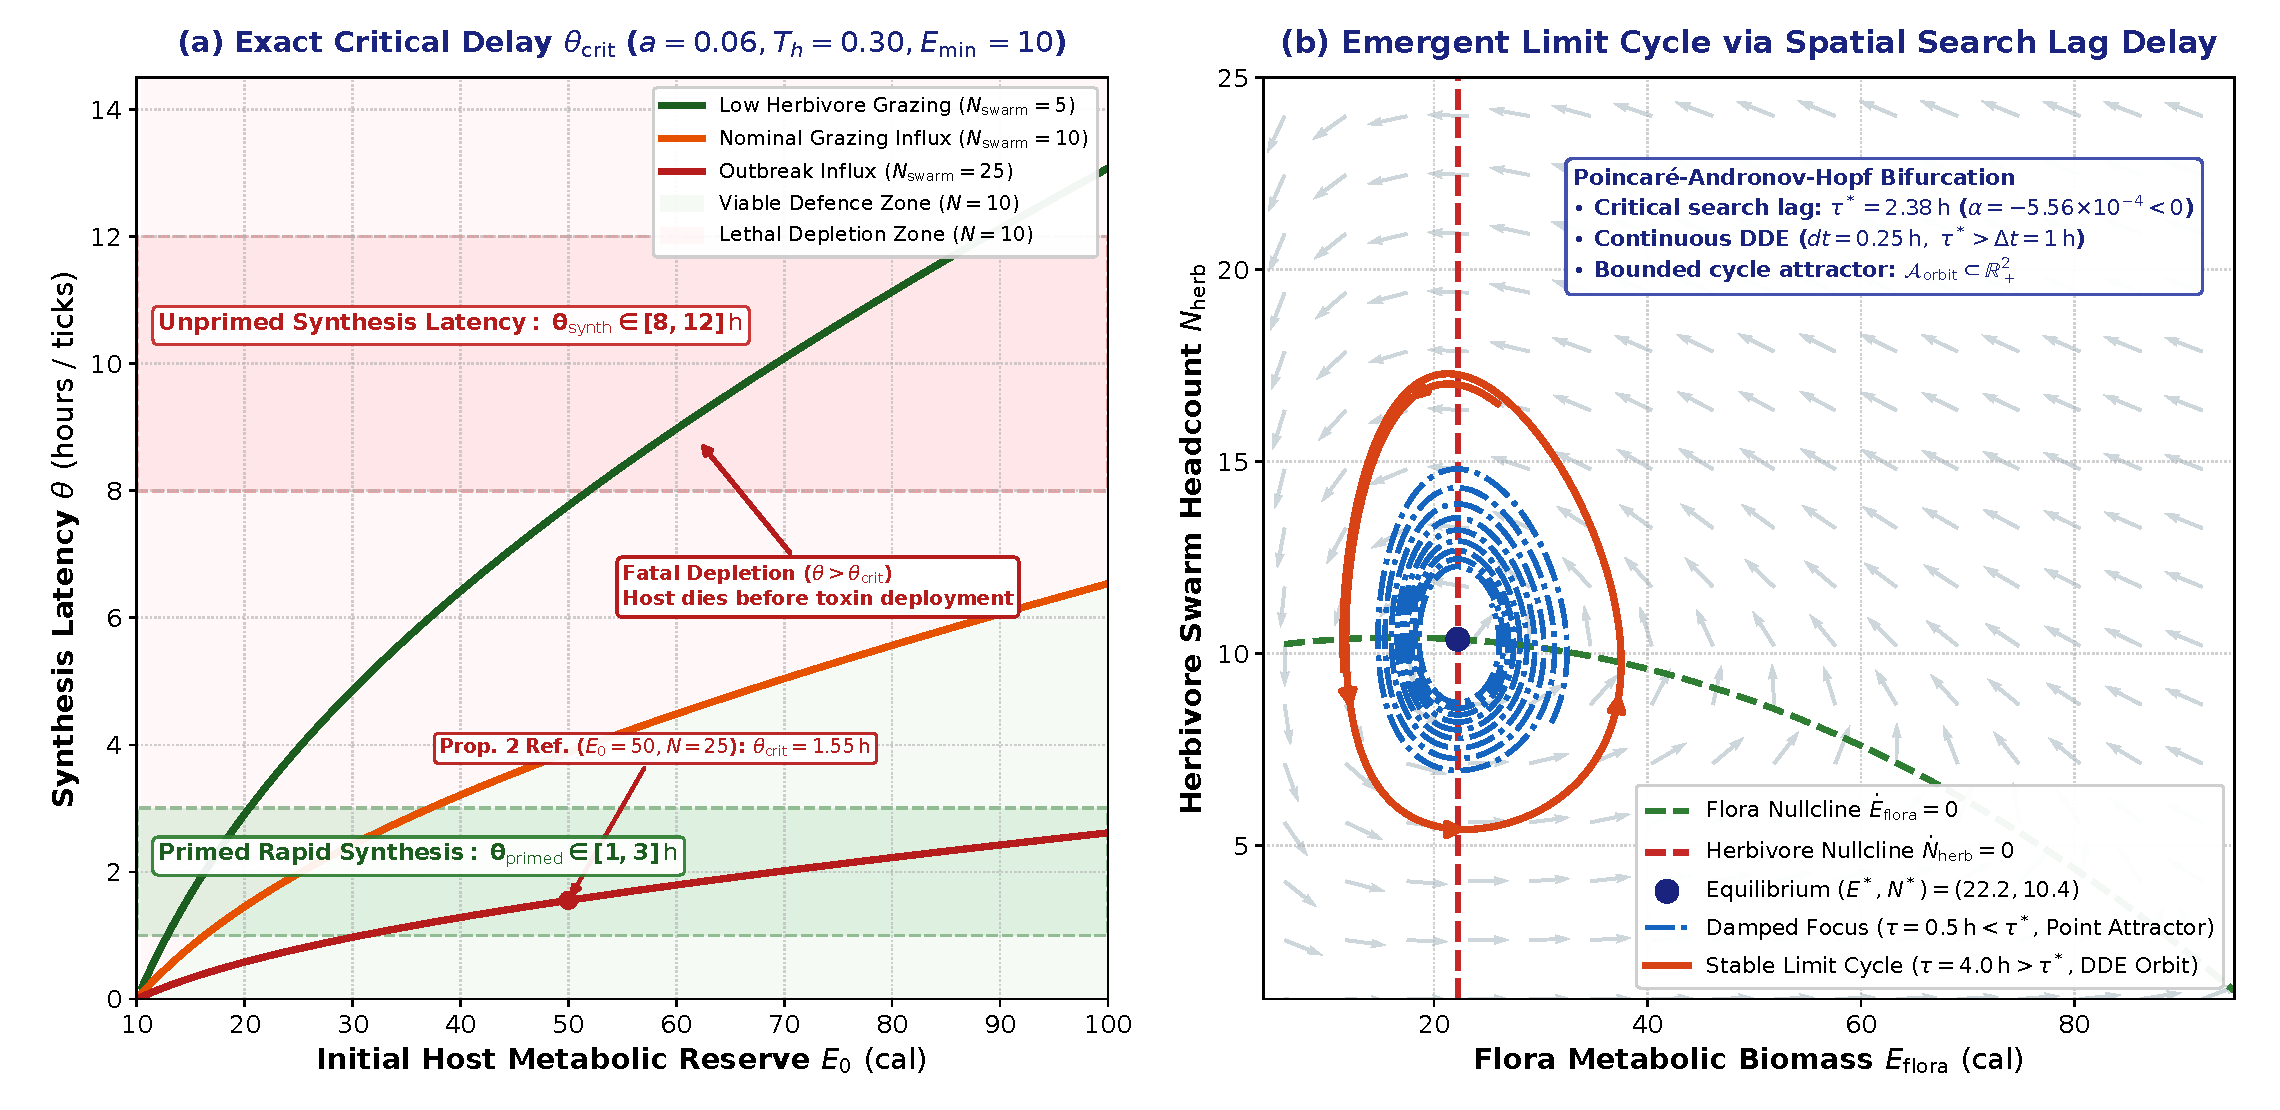
\includegraphics[width=0.92\textwidth]{figures/fig06_limit_cycle_bifurcation.pdf}

  \caption{Analytical Stability Boundaries and Mean-Field Delay Bifurcation Surfaces. (a) Critical synthesis latency bound $\theta_{\mathrm{crit}}$ as a function of initial host metabolic reserve $E_0$ and co-located grazing pressure $N_{\mathrm{swarm}}$ under continuous hourly intake. The shaded region separates the parameter zone in which pre-primed synthesis ($\theta_{\mathrm{primed}} < \theta_{\mathrm{crit}}$) preserves the host above $E_{\min}$ from the zone of lethal depletion. (b) Phase portrait in the $(E_{\mathrm{flora}}, N_{\mathrm{herb}})$ plane for the time-scaled delayed Rosenzweig--MacArthur system ($r = 0.02\,\mathrm{h}^{-1}$, $a = 0.002\,\mathrm{cell}^{-1}\mathrm{h}^{-1}$, $T_h = 7.5\,\mathrm{h}$, $e_{\mathrm{eff}} = 0.60$, $m_{\mathrm{herb}} = 0.02\,\mathrm{h}^{-1}$, $K = 100.0\,\mathrm{cal}$), illustrating convergence to a damped focus at $\tau = 0.5\,\mathrm{h} < \tau^*$ and a bounded limit cycle $\mathcal{A}_{\mathrm{orbit}}$ at $\tau = 4.0\,\mathrm{h} > \tau^* = 2.38\,\mathrm{h}$.}
  \label{fig:limit_cycle_bifurcation}
\end{figure*}

% ==============================================================================
\subsection{Capacity Bound and Non-Reproductive Dissipation}
\label{subsec:thermodynamic_conservation}
% ==============================================================================

Let $\mathcal{E}_t^{\mathrm{flora}} \subseteq \Lambda$ denote the set of active plant entities (at most one per lattice coordinate $(x, y) \in \Lambda$, carrying energy $E_i(t) \in [0, E_{\max}]$) and $\mathcal{S}_t^{\mathrm{herb}}$ the active herbivore swarms ($E_j^{\mathrm{herb}}(t) \le E_{\max}^{\mathrm{swarm}}$, bounded per tile by $C_{\max}$ so global swarm count satisfies $|\mathcal{S}_t^{\mathrm{herb}}| \le |\Lambda| C_{\max}$). Aggregate active somatic and swarm energy is defined as:
\begin{equation}
  \mathcal{H}_{\mathrm{biotope}}(t) \coloneqq \sum_{i \in \mathcal{E}_t^{\mathrm{flora}}} E_i(t) + \sum_{j \in \mathcal{S}_t^{\mathrm{herb}}} E_j^{\mathrm{herb}}(t).
  \label{eq:aggregate_energy_def}
\end{equation}

\begin{proposition}[Capacity Bound and Non-Reproductive Dissipation]
\label{prop:capacity_boundedness}
Under the coupled transition operators of PHIDS:
\begin{enumerate}
  \item \textbf{Capacity Ceiling:} For all ticks $t \ge 0$, aggregate active energy remains bounded by finite lattice capacity: $\mathcal{H}_{\mathrm{biotope}}(t) \le |\Lambda| E_{\max} + |\mathcal{S}_{\max}| E_{\max}^{\mathrm{swarm}} < \infty$.
  \item \textbf{Non-Reproductive Metabolic Dissipation:} On any tick without photosynthetic influx ($\Phi_{\mathrm{photo}}(t) = 0$) and without seedling germination events (or globally for parameterisations satisfying $E_{\mathrm{seed}} \ge E_{\mathrm{base}}$), net total energy is non-increasing, $\Delta \mathcal{H}_{\mathrm{biotope}}(t) \le -\Phi_{\mathrm{struct}}(t) - \Phi_{\mathrm{myco}}(t) - \Phi_{\mathrm{resp}}(t) - \Phi_{\mathrm{def}}(t) - \Phi_{\mathrm{waste}}(t) \le 0$, with strict dissipation ($\Delta \mathcal{H}_{\mathrm{biotope}}(t) < 0$) whenever mature structural flora ($M_i > 0$), active herbivores, active inducible defences, or mycorrhizal links exist on the evaluated step.
\end{enumerate}
\end{proposition}

\begin{proof}
Because at most one plant occupies each grid cell, $|\mathcal{E}_t^{\mathrm{flora}}| \le |\Lambda|$, and growth saturates via $E_i(t+1) = \min(E_{\max}, E_i(t) + \Delta E_{\mathrm{growth},i})$. Swarm occupancy per cell is masked at capacity $C_{\max}$ and binary fission halves parent energy ($E_{\mathrm{child}} = E_{\mathrm{parent}}/2$), establishing Part~1. For Part~2, grazing extracts $\Delta E_{\mathrm{grazed}}$ with net assimilated fraction $\tilde{e}_{\mathrm{eff}} = (1 - \delta_{\mathrm{morph}}) e_{\mathrm{eff}} \in (0, 1)$, dissipating $\Phi_{\mathrm{waste}} = (1 - \tilde{e}_{\mathrm{eff}})\Delta E_{\mathrm{grazed}} \ge 0$; enzyme synthesis deducts $\Phi_{\mathrm{def}} = \sum c_{\mathrm{synth}} \ge 0$, mycorrhizal establishment and weekly link upkeep deduct $\Phi_{\mathrm{myco}} \ge 0$, plant cohorts with $M_i > 0$ deduct structural maintenance $\Phi_{\mathrm{struct}} = \sum 0.5\,E_{\min}\,(M_i / M_{\max}) \ge 0$, and diurnal active herbivores deduct basal respiration $\Phi_{\mathrm{resp}} \ge 0$ (while resetting negative energy after integer starvation deductions via Eq.~\eqref{eq:integer_casualty_clearing}). Setting $\Phi_{\mathrm{photo}} = 0$ leaves $\Delta \mathcal{H}_{\mathrm{biotope}} \le 0$ whenever germination either adds no energy ($E_{\mathrm{seed}} \ge E_{\mathrm{base}}$) or is absent on the step, and strictly negative whenever any dissipation channel acts (newly germinated seedlings carry $M_i = 0$ and zero links until their first active structural cohort). When parameterisations set $E_{\mathrm{base}} > E_{\mathrm{seed}}$ (Table~\ref{tab:case_study_configurations}), each germination introduces an establishment-carbon subsidy $E_{\mathrm{base}} - E_{\mathrm{seed}} > 0$ representing seedbank reserves, remaining globally bounded by Part~1.
\end{proof}

% ==============================================================================
\subsection{Continuous-Grazing Critical Synthesis Delay}
\label{subsec:critical_synthesis_delay}
% ==============================================================================

Unprimed plants incur a physiological synthesis delay $\theta_{\mathrm{synth}}$ --- encompassing elicitor perception, jasmonate signalling, and enzymatic translation --- before inducible toxins become active. Consider a single host plant with initial reserve $E_0 > E_{\min}$ at $t = 0$ subjected to a worst-case continuous per-tick feeding regime (applying the per-event functional response Eq.~\eqref{eq:math_holling_type_ii} at every hourly step $\Delta t = 1\,\text{h}$ with movement period $v = 1$, rather than on $24$-tick diurnal strides) by a co-located swarm of size $N_{\mathrm{swarm}}$:
\begin{equation}
  \dot{E}_{\mathrm{loss}}(E) = \frac{a E}{1 + a T_h E} \cdot N_{\mathrm{swarm}},
  \label{eq:intake_ode}
\end{equation}
where $a$ is the effective per-event attack rate and $T_h$ the handling time per unit biomass. Unprimed hosts experience $\theta_{\mathrm{synth}} \in [8, 12]\,\text{h}$ without chemical deterrence ($\delta_{\mathrm{chem}} = 0$) over $t \in [0, \theta_{\mathrm{synth}})$. If $E(t)$ falls below $E_{\min}$ prior to deployment, $\mathcal{T}_{\text{interact}}$ removes the host before toxins take effect. Eq.~\eqref{eq:intake_ode} defines a worst-case continuous-grazing lower bound corresponding to sustained hourly multi-swarm arrival; under $24$-tick diurnal strides, single-swarm grazing buffers moderate delays ($\theta_{\mathrm{synth}} \le 24\,\text{h}$) unless the initial grazing event depletes the host below $E_{\min}$.

\begin{proposition}[Continuous-Grazing Critical Synthesis Delay $\theta_{\mathrm{crit}}$]
\label{thm:critical_synthesis_delay}
Let a host plant have initial reserve $E_0 > E_{\min}$ under continuous hourly grazing governed by \eqref{eq:intake_ode}. The closed-form critical synthesis delay threshold $\theta_{\mathrm{crit}}$ separating host survival from deterministic mortality is:
\begin{equation}
  \theta_{\mathrm{crit}} \coloneqq \frac{1}{N_{\mathrm{swarm}}} \left[ \frac{1}{a} \ln\left(\frac{E_0}{E_{\min}}\right) + T_h (E_0 - E_{\min}) \right].
  \label{eq:theta_crit_exact}
\end{equation}
Accordingly:
\begin{enumerate}
  \item If $\theta_{\mathrm{synth}} > \theta_{\mathrm{crit}}$, unprimed host mortality occurs deterministically at $t^* = \theta_{\mathrm{crit}}$ prior to toxin deployment.
  \item If priming compresses synthesis latency to $\theta_{\mathrm{primed}} < \theta_{\mathrm{crit}}$, inducible defences activate before $E(t)$ reaches $E_{\min}$.
\end{enumerate}
\end{proposition}

\begin{proof}
Separating variables in $\frac{dE}{dt} = -\frac{a E}{1 + a T_h E} N_{\mathrm{swarm}}$ and integrating from $E(0) = E_0$ to $E(t)$ gives:
\begin{equation}
  \frac{1}{a} \ln\left(\frac{E(t)}{E_0}\right) + T_h \left(E(t) - E_0\right) = - N_{\mathrm{swarm}} \cdot t.
  \label{eq:integrated_depletion}
\end{equation}
Setting $E(t^*) = E_{\min}$ yields $t^* \equiv \theta_{\mathrm{crit}}$ directly as in \eqref{eq:theta_crit_exact}.
\end{proof}

\begin{remark}[Baseline Priming Regime]
For a reference host parameterised at $E_0 = 50\,\text{cal}$, $E_{\min}=10\,\text{cal}$, $a=0.06\,\text{cell}^{-1}\text{h}^{-1}$, and $T_h=0.30\,\text{h}$ under sustained grazing ($N_{\mathrm{swarm}} \geq 5$), nominal unprimed delays ($\theta_{\mathrm{synth}} \in [8, 12]\,\text{h}$) exceed $\theta_{\mathrm{crit}}$ (Fig.~\ref{fig:limit_cycle_bifurcation}a), whereas primed delays $\theta_{\mathrm{primed}} \in [1, 3]\,\text{h}$ lie inside the survival region across low to moderate swarm densities.
\end{remark}

% ==============================================================================
\subsection{Mean-Field Delay-Bifurcation Criterion}
\label{subsec:hopf_limit_cycle}
% ==============================================================================

Lumped predator--prey ODEs \cite{rosenzweig1963graphical} assume instantaneous spatial encounter. In lattice biotopes, herbivores incur finite transit lag moving between host patches as well as trophic assimilation lag. To isolate how spatial-trophic delay alters local stability in the undefended baseline prior to inducible defences, we project the baseline consumer--resource interaction onto a continuous-time mean-field delay differential equation (DDE) system:
\begin{align}
  \frac{dE}{dt} &= r E(t) \left(1 - \frac{E(t)}{K}\right) - \frac{a E(t)}{1 + a T_h E(t)} N(t), \label{eq:dde_flora} \\
  \frac{dN}{dt} &= e_{\mathrm{eff}} \frac{a E(t - \tau)}{1 + a T_h E(t - \tau)} N(t) - m_{\mathrm{herb}} N(t), \label{eq:dde_herb}
\end{align}
where $\tau \coloneqq \tau_{\mathrm{lag}} > 0$ denotes the effective spatial-search and trophic assimilation lag ($\tau_{\mathrm{spatial}} = \bar{d}_{\mathrm{patch}} / v_{\mathrm{eff}}$ plus digestive assimilation delay) of the undefended Rosenzweig--MacArthur baseline. The non-trivial coexistence equilibrium $(E^*, N^*)$ satisfies $\frac{dE}{dt} = \frac{dN}{dt} = 0$:
\begin{align}
  E^* &= \frac{m_{\mathrm{herb}}}{a (e_{\mathrm{eff}} - m_{\mathrm{herb}} T_h)}, \label{eq:interior_equilibrium_e} \\
  N^* &= \frac{r}{a}\left(1 - \frac{E^*}{K}\right)(1 + a T_h E^*). \label{eq:interior_equilibrium_n}
\end{align}
Choosing realistic hourly growth and mortality rates ($r = 0.02\,\text{h}^{-1}$, $K = 100.0\,\text{cal}$, $a = 0.002\,\text{cell}^{-1}\text{h}^{-1}$, $T_h = 7.5\,\text{h}$, $e_{\mathrm{eff}} = 0.60$, $m_{\mathrm{herb}} = 0.02\,\text{h}^{-1}$), Eqs.~\eqref{eq:interior_equilibrium_e}--\eqref{eq:interior_equilibrium_n} yield $(E^*, N^*) = (22.22\,\text{cal}, 10.37)$ to the right of the Rosenzweig--MacArthur nullcline hump ($E_{\mathrm{hump}} = 16.67\,\text{cal}$), ensuring local asymptotic stability ($\alpha = -5.56 \times 10^{-4} < 0$) at $\tau = 0$ and a Hopf bifurcation above the engine step size at $\tau^* = 2.38\,\text{h} > \Delta t = 1.0\,\text{h}$ (Fig.~\ref{fig:limit_cycle_bifurcation}b).

\begin{proposition}[Mean-Field Delay-Bifurcation Criterion]
\label{thm:hopf_limit_cycle}
Let $E^* < K$ such that an interior equilibrium $(E^*, N^*)$ exists, and let the linearised Jacobian of \eqref{eq:dde_flora}--\eqref{eq:dde_herb} about $(E^*, N^*)$ be given by:
\begin{equation}
  J_0 = \begin{pmatrix} \alpha & -\beta \\ 0 & 0 \end{pmatrix}, \quad J_\tau = \begin{pmatrix} 0 & 0 \\ \gamma & 0 \end{pmatrix},
\end{equation}
with $\alpha = r\left(1 - \frac{2E^*}{K}\right) - \frac{a N^*}{(1 + a T_h E^*)^2}$, $\beta = \frac{a E^*}{1 + a T_h E^*}$, and $\gamma = \frac{e_{\mathrm{eff}} a N^*}{(1 + a T_h E^*)^2}$. When $p = -\alpha > 0$, there exists a critical delay $\tau^*$ such that:
\begin{enumerate}
  \item For $\tau < \tau^*$, $(E^*, N^*)$ is locally asymptotically stable.
  \item At $\tau = \tau^*$, a pair of simple conjugate eigenvalues crosses the imaginary axis transversally (Poincaré--Andronov--Hopf bifurcation).
  \item For $\tau > \tau^*$, $(E^*, N^*)$ is linearly unstable and a periodic orbit branch bifurcates at $\tau^*$.
\end{enumerate}
The critical delay is:
\begin{equation}
  \tau^* = \frac{1}{\omega_0} \arccos\left( \frac{\omega_0^2}{r_{\mathrm{delay}}} \right),
  \label{eq:tau_star_exact}
\end{equation}
where $\omega_0 = \sqrt{\frac{-p^2 + \sqrt{p^4 + 4 r_{\mathrm{delay}}^2}}{2}}$ is the positive root of $\omega^4 + p^2\omega^2 - r_{\mathrm{delay}}^2 = 0$ with $r_{\mathrm{delay}} = \beta \gamma$.
\end{proposition}

\begin{proof}
Linearising \eqref{eq:dde_flora}--\eqref{eq:dde_herb} yields the characteristic quasipolynomial $\mathcal{D}(\lambda, \tau) = \lambda^2 + p\lambda + r_{\mathrm{delay}} e^{-\lambda\tau} = 0$ ($p = -\alpha > 0$, $r_{\mathrm{delay}} = \beta\gamma > 0$). Substituting $\lambda = i\omega$ ($\omega > 0$) gives $\omega^2 = r_{\mathrm{delay}}\cos(\omega\tau)$ and $p\omega = r_{\mathrm{delay}}\sin(\omega\tau)$, eliminating $\tau$ to yield $\omega^4 + p^2\omega^2 - r_{\mathrm{delay}}^2 = 0$, unique positive root $\omega_0$, and $\tau^*$ in \eqref{eq:tau_star_exact}. Implicit differentiation at $\lambda = i\omega_0$ yields $\operatorname{Re}\!\left[\left.(d\lambda/d\tau)^{-1}\right|_{\tau=\tau^*}\right] = (2\omega_0^2 + p^2)/r_{\mathrm{delay}}^2 > 0$, verifying transversal crossing.
\end{proof}

\begin{remark}[Numerical Verification and Diagnostic Role]
At the time-scaled reference parameters above, numerical DDE integration (Fig.~\ref{fig:limit_cycle_bifurcation}b) confirms a damped spiral focus at $\tau = 0.5\,\mathrm{h} < \tau^*$ and convergence onto a bounded limit cycle $\mathcal{A}_{\mathrm{orbit}} \subset \mathbb{R}_+^2$ at $\tau = 4.0\,\mathrm{h} > \tau^* = 2.38\,\mathrm{h}$. In calibrated multi-species runs where $E^* < E_{\mathrm{hump}}$ ($\alpha > 0$ at $\tau = 0$; Section~\ref{sec:ecotone_theorem_parity}), the lumped DDE prerequisite $p > 0$ is violated, diagnosing that coexistence depends on spatial dispersal and multi-guild resource partitioning rather than local ODE equilibrium stability.
\end{remark}


% ==============================================================================
% Section 6: In-Silico Case Studies & Dynamic Trajectory Analysis
% ==============================================================================
% ==============================================================================
% Section 6: In-Silico Case Study (Central European Ecotone)
% ==============================================================================

\section{In-Silico Case Study: Central European Riparian-to-Floodplain-Meadow Ecotone}
\label{sec:case_studies}

To evaluate the coupled hybrid dynamical engine under multi-trophic heterogeneity, we construct and analyse a meso-scale \textbf{Central European Riparian-Woodland to Floodplain-Meadow Ecotone} on a $256 \times 256\,\text{m}$ ($6.55\,\text{ha}$, $1\,\text{m}^2$ per cell) periodic torus over a $4{,}000$-tick ($166.7$-day) temperate growing season. Four linked experiments examine the framework: (i) zero-shot spatial scale transfer ($128 \times 64 \to 256 \times 256$) and $10$-seed single-season community persistence, (ii) diagnostic evaluation of Propositions~\ref{thm:critical_synthesis_delay} and~\ref{thm:hopf_limit_cycle} under runtime kinetics, (iii) factorial wind and dual-channel ablation paired with a deterministic upwind relay experiment, and (iv) variance-based global sensitivity analysis with Common Random Numbers (CRN) across two spatial scales.

% ==============================================================================
\subsection{Ecological Context, Selection Rationale, and Biotope Construction}
\label{sec:ecotone_design}
% ==============================================================================

The modelled community represents lowland Central European river floodplains --- specifically the Oder and Elbe basins, including Brandenburg alluvial corridors --- where softwood riparian galleries (\textit{Salix}--\textit{Populus} stands and \textit{Ficario}--\textit{Ulmetum minoris} edges) grade into mesic floodplain grasslands (\textit{Arrhenatherion} meadows) and disturbed alluvial verges \cite{leuschner2017ecology, leuschner2017nonforest}. Prevailing summer airflow along WSW$\to$ENE ($22.5^\circ$) places the riparian fringe upwind on the western bank and the alluvial meadow downwind in the east. On the hourly lattice step, the wind vector $\mathbf{u}_{\text{wind}} = (0.878, 0.364)\,\text{cells/tick}$ ($\|\mathbf{u}_{\text{wind}}\| = 0.95\,\text{cells/tick}$) serves as the effective hourly plume-drift proxy defined in Section~\ref{subsec:atmospheric_transport} (scaling bounds are examined in Section~\ref{subsec:model_limitations}). Within $1\,\text{m}^2$ cells, woody taxa ($p_0, p_1$) represent juvenile floodplain saplings or clonal ramet patches whose reproduction intervals ($1{,}303\text{--}1{,}737\,\text{ticks}$) compress clonal recruitment into a single growing season, while herbivore guilds represent folivorous larval aggregations ($h_0, h_1, h_3, h_4$) and wingless aphid colonies ($h_2$) stepping at integer periods $v \in \{1, 2, 3\}\,\text{ticks/step}$.

Whereas simplified three-species orchard configurations omit growth--defence hierarchies, constitutive abrasion, inter-species root conduits, specialist counter-adaptations, and an embedded non-mycorrhizal control, the ecotone exercises every PHIDS mechanism inside its fixed 16-channel array layout ($6$ flora guilds, $5$ herbivore guilds, $9$ chemical channels $s_0$--$s_8$; Table~\ref{tab:case_study_configurations}). Six flora guilds span the growth--defence continuum: \textit{Populus nigra} ($p_0$, inducible green leaf volatile and terpenoid emitter with rapid vascular phloem withdrawal \cite{babst2005jasmonic, frost2008priming}); \textit{Salix purpurea} ($p_1$, high constitutive lignified and salicinoid armour \cite{boeckler2011phenolic, kayser2025pharmaceutical}); \textit{Trifolium repens} ($p_2$, high-degree arbuscular mycorrhizal hub with inducible cyanogenic glycosides and phloem withdrawal \cite{babikova2013underground, olsen2021dual, shen2023between, li2025common}); \textit{Lolium perenne} ($p_3$, constitutive silica phytoliths plus CMN-primed polyphenol oxidase escalation \cite{massey2006silica, shen2023between, li2025common}); \textit{Tanacetum vulgare} ($p_4$, aromatic ecotone fringe combining olfactory camouflage $\Phi_{\text{camo}}$ with proactive terpenoid deterrence \cite{clancy2016chemotypic}); and \textit{Brassica nigra} ($p_5$, non-mycorrhizal ruderal pioneer providing an embedded zero-CMN control \cite{schreiner1993stimulation, bekaert2012metabolic}).

Five herbivore guilds pair host specialisation with biochemical counter-adaptations: \textit{Lymantria dispar} ($h_0$, woody defoliator on $p_0, p_1$ \cite{lindroth2024forest}); \textit{Phratora vitellinae} ($h_1$, Salicaceae specialist tolerant of salicin \cite{pasteels1983salicin, kuhn2004selective}); \textit{Acyrthosiphon pisum} ($h_2$, phloem-feeding colony on $p_2$ \cite{shih2023pea}); \textit{Noctua pronuba} ($h_3$, polyphagous meadow generalist across $p_2$--$p_5$ \cite{topping2025noctua}); and \textit{Pieris brassicae} ($h_4$, crucifer specialist on $p_5$ whose nitrile-specifier proteins disarm allyl isothiocyanate escalation \cite{okamura2022testing}, realised in PHIDS by gating $s_7$ emission strictly to generalist $h_3$ feeding). Across the flora ($31$ trigger rules total), $10$ primary attack triggers initiate Stage-1 signalling, $3$ conditional rules govern phloem withdrawal on $p_0$--$p_2$, and $18$ conditionally gated rules coordinate secondary VOC relays and inducible toxins across riparian airborne priming ($s_0 \to s_1 \to s_3/s_4$), upwind meadow CMN relays ($s_2 \to s_6/s_8$), proactive $p_4$ deterrence ($s_5$), and generalist-gated $p_5$ escalation ($s_7$). All lethal toxins require composite priming-plus-grazing predicates, preventing unconditional firing on unattacked tiles.

Spatially, the ecotone is arranged across four overlapping habitat zones from west to east under the prevailing WSW$\to$ENE airflow (Table~\ref{tab:ecotone_spatial_init}, Fig.~\ref{fig:ecotone_spatial_snapshot}a). Thomas cluster processes establish upwind riparian galleries of \textit{Populus nigra} and \textit{Salix purpurea} across the western terrace and downwind meadow stands of \textit{Trifolium repens} and \textit{Lolium perenne} across the eastern floodplain. Between them, a bimodal inhomogeneous Poisson intensity creates an aromatic transition fringe of \textit{Tanacetum vulgare} centred near the woodland margin ($x = 112$) and the western edge ($x = 16$). Finally, thinned circular micro-patches of \textit{Brassica nigra} occupy alluvial gaps and woodland clearings under checkerboard parity and strict cardinal-neighbour exclusion, enforcing zero mycorrhizal connectivity ($\overline{\deg}_{\text{CMN}}(p_5) = 0.00$) alongside $61.9\%$--$85.4\%$ initial connectivity across $p_0$--$p_4$. Initialisation places $14{,}679$ plants ($22.40\%$ cover) and $72$ founder swarms ($1{,}554$ individuals) on the $256 \times 256$ flagship lattice, and $1{,}941$ plants ($23.69\%$ cover) with $20$ founder swarms ($208$ individuals) on the $128 \times 64$ calibration twin. Figure~\ref{fig:ecotone_spatial_snapshot} shows a live state snapshot at tick $331$ together with a $56 \times 56$ transition detail resolving individual cardinal root links, herbivore swarms, and downwind VOC plumes.

\begin{figure*}[t]
  \centering
  % ==============================================================================
% Figure 6 (LaTeX fig08): Spatial Ecotone Snapshot & Zoomed Transition ROI
% ==============================================================================

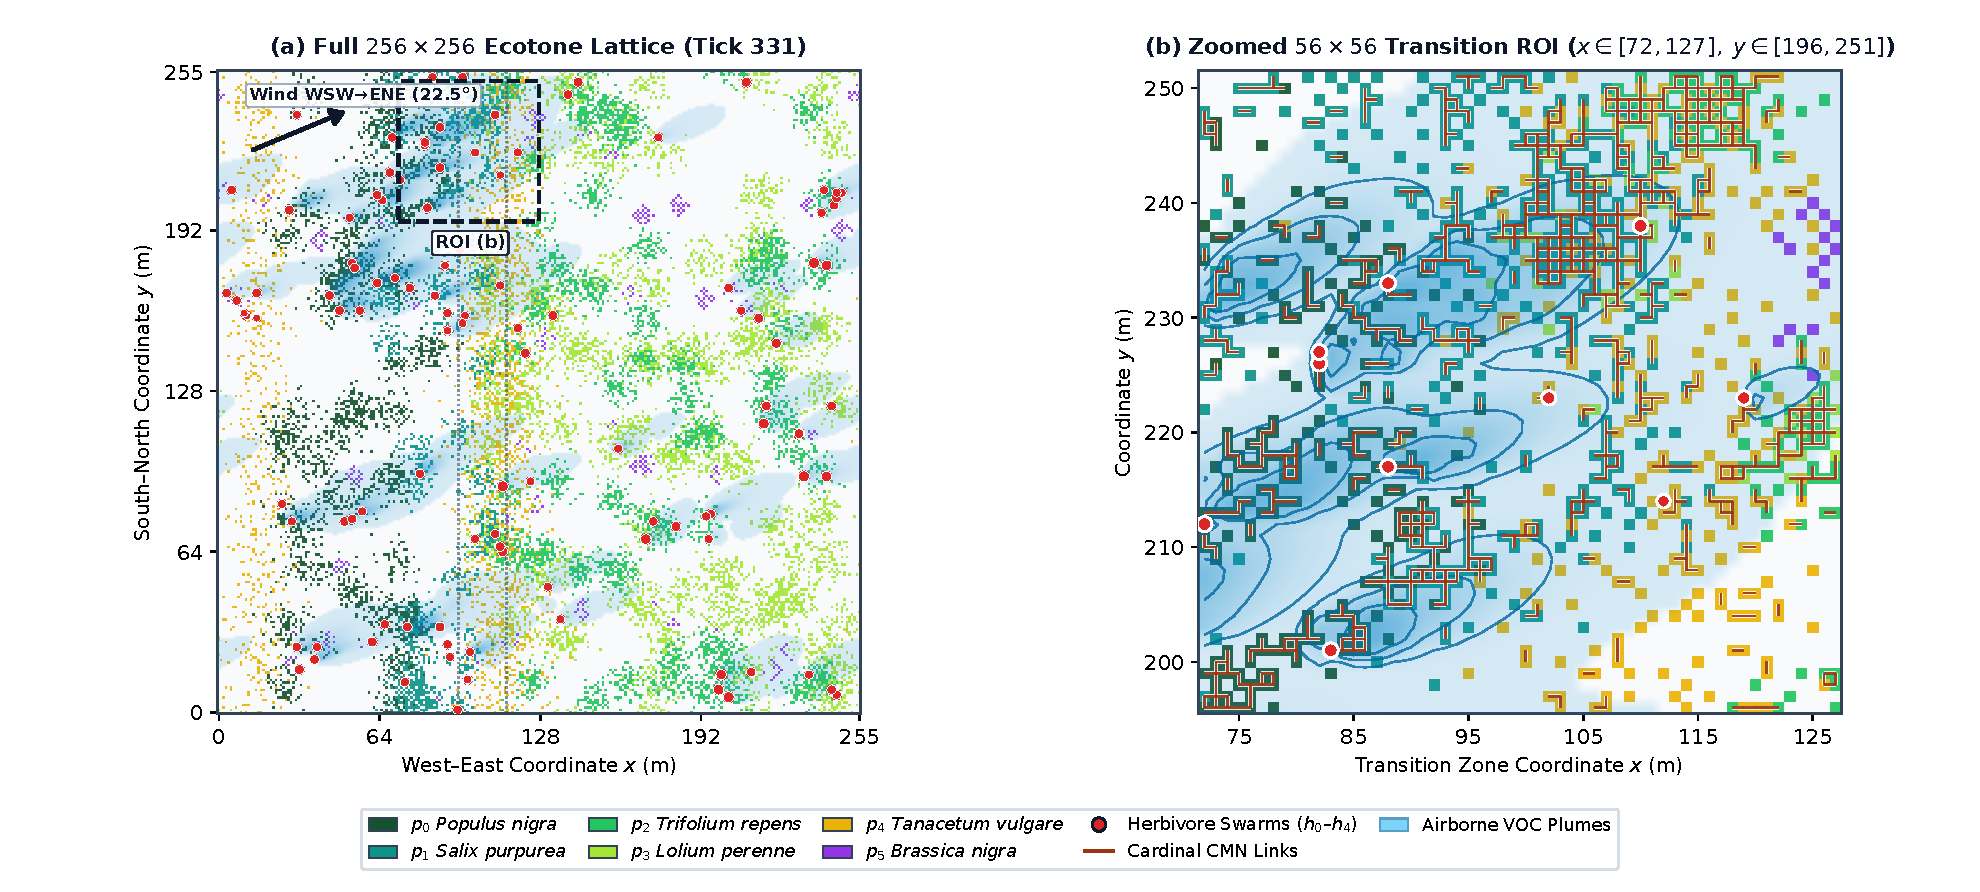
\includegraphics[width=\textwidth]{figures/fig08_ecotone_spatial_snapshot.pdf}

  \caption{Spatial State Snapshot of the Calibrated $256 \times 256$ Central European Ecotone at Tick $331$ ($13{,}880$ active plants, $128$ herbivore swarms comprising $3{,}867$ individuals, and $10{,}331$ undirected cardinal mycorrhizal links). \textbf{(a)} Full $256 \times 256\,\mathrm{m}$ lattice showing upwind western riparian woodland ($p_0, p_1$), the aromatic \textit{Tanacetum} transition fringe ($p_4$), the downwind eastern meadow ($p_2, p_3$), isolated non-mycorrhizal \textit{Brassica nigra} patches ($p_5$), airborne VOC plumes ($C_{s_0\text{--}s_2}$), and herbivore swarms under WSW$\to$ENE ($22.5^\circ$) plume drift. \textbf{(b)} Zoomed $56 \times 56$ transition window ($x \in [72, 128)$, $y \in [196, 252)$; $1{,}020$ plants, $11$ swarms, $868$ interior cardinal root links) resolving cell-level guild boundaries, explicit mycorrhizal edges, and local VOC dispersion contours.}
  \label{fig:ecotone_spatial_snapshot}
\end{figure*}

\begin{table*}[b]
\caption{Spatial Point-Process Initialisation Parameters and Initial Cardinal Mycorrhizal Connectivity on the $256 \times 256$ Ecotone.}
\label{tab:ecotone_spatial_init}
\vspace{4pt}
\centering
\scriptsize
\setlength{\tabcolsep}{2.5pt}
\begin{tabularx}{\textwidth}{
  >{\raggedright\hsize=1.08\hsize}X
  >{\raggedright\hsize=0.90\hsize}X
  >{\centering\hsize=0.82\hsize}X
  >{\centering\hsize=0.80\hsize}X
  >{\raggedright\hsize=1.10\hsize}X
  >{\raggedright\hsize=1.10\hsize}X
  >{\raggedright\arraybackslash\hsize=1.20\hsize}X
}
\toprule
\textbf{Flora Guild} & \textbf{Spatial Process} & \textbf{Domain Band ($x$)} & \textbf{Parents / Patches} & \textbf{Intensity / Offspring} & \textbf{Dispersion / Exclusion} & \textbf{Initial $N_0$ / CMN Conn.} \\
\midrule
$p_0$ \textit{Populus nigra}     & Thomas cluster & $x \in [22, 88]$   & $55$ parents & $\mathrm{Poisson}(65)$ & $\sigma_r = 4.2\,\mathrm{m}$ & $2{,}755$ ($78.3\%$, $\overline{\deg}=1.59$) \\
$p_1$ \textit{Salix purpurea}    & Thomas cluster & $x \in [66, 110]$  & $42$ parents & $\mathrm{Poisson}(55)$ & $\sigma_r = 3.8\,\mathrm{m}$ & $1{,}698$ ($85.0\%$, $\overline{\deg}=1.87$) \\
$p_2$ \textit{Trifolium repens}  & Thomas cluster & $x \in [114, 244]$ & $65$ parents & $\mathrm{Poisson}(75)$ & $\sigma_r = 3.6\,\mathrm{m}$ & $3{,}552$ ($85.4\%$, $\overline{\deg}=1.88$) \\
$p_3$ \textit{Lolium perenne}    & Thomas cluster & $x \in [106, 248]$ & $85$ parents & $\mathrm{Poisson}(70)$ & $\sigma_r = 4.5\,\mathrm{m}$ & $4{,}346$ ($76.6\%$, $\overline{\deg}=1.48$) \\
$p_4$ \textit{Tanacetum vulgare} & Bimodal inh.\ Poisson & Peaks $x = 112, 16$ & $2$ Gaussian bands & $p_{\max} = 0.24, 0.14$ (cap $0.35$) & $\sigma = 9, 7\,\mathrm{m}$ & $1{,}871$ ($61.9\%$, $\overline{\deg}=1.11$) \\
$p_5$ \textit{Brassica nigra}    & Thinned micro-patches & $48$ gap / $12$ core & $60$ discs ($r = 4$) & Checkerboard ($p = 0.72$) & Zero cardinal neighbours & $457$ ($0.0\%$, $\overline{\deg}=0.00$) \\
\bottomrule
\multicolumn{7}{@{}p{\textwidth}@{}}{Flagship $256 \times 256$ initialisation yields $14{,}679$ plants ($22.40\%$ cover) and $72$ founder swarms ($1{,}554$ individuals). The $128 \times 64$ reduced-lattice calibration twin scales parent and patch counts proportionally to lattice area ($1{,}941$ plants, $23.69\%$ cover, $20$ founder swarms comprising $208$ individuals).}
\end{tabularx}
\end{table*}

% ==============================================================================
% Table 4 (LaTeX tab07): Calibrated Central European Ecotone Parameterisation
% Placed at bottom [b] of page, caption above table
% ==============================================================================

\begin{table*}[b]
\caption{Calibrated Parameterisation of the Central European Riparian-to-Floodplain-Meadow Ecotone ($256 \times 256$ Flagship and $128 \times 64$ Reduced-Lattice Twin).}
\label{tab:case_study_configurations}
\vspace{4pt}
\centering
\scriptsize
\setlength{\tabcolsep}{1.6pt}
\begin{tabular*}{\textwidth}{@{\extracolsep{\fill}} l c c c c c c c c @{}}
\toprule
\multicolumn{9}{@{}l}{\textbf{Panel A: Six Sympatric Flora Guilds ($p_0$--$p_5$)} --- Cohort growth $r_p$, seed dist.\ $[d_{\min},d_{\max}]$ ($p_0{:}6\text{--}28$, $p_1{:}5\text{--}22$, $p_2{:}1\text{--}5$, $p_3{:}1\text{--}8$, $p_4{:}1\text{--}6$, $p_5{:}1\text{--}4$)} \\
\midrule
\textbf{Flora Species} &
\textbf{$E_{\mathrm{b}}/E_{\max}/E_{\min}$} &
\textbf{$r_p$} &
\textbf{Repro / $E_{\text{seed}}$} &
\textbf{$c_{\text{bite}}$ / $(1{-}\delta_m)$} &
\textbf{$\Phi_{\text{camo}}$} &
\textbf{$\eta_{\min}$ / $\gamma_{\text{tr}}$} &
\textbf{$\delta_E^{\text{tax}}$} &
\textbf{$N_0$ / $\overline{\deg}_{\text{CMN}}$} \\
\midrule
$p_0$ \textit{Populus nigra}     & $70/140/14$ & $0.1500$ & $1303$ / $56.00$ & $0.05$ / $0.88$ & $1.00$ & $0.45$ / $0.08$ & $0.65$ & $2{,}755$ / $1.59$ \\
$p_1$ \textit{Salix purpurea}    & $60/120/12$ & $0.0935$ & $1737$ / $48.00$ & $0.15$ / $0.62$ & $1.00$ & $0.70$ / $0.05$ & $0.55$ & $1{,}698$ / $1.87$ \\
$p_2$ \textit{Trifolium repens}  & $45/85/9$   & $0.3000$ & $1086$ / $34.15$ & $0.00$ / $0.96$ & $1.00$ & $0.55$ / $0.10$ & $0.50$ & $3{,}552$ / $1.88$ \\
$p_3$ \textit{Lolium perenne}    & $55/105/11$ & $0.3200$ & $1086$ / $42.69$ & $0.22$ / $0.68$ & $1.00$ & $---$ / $0.06$  & $0.50$ & $4{,}346$ / $1.48$ \\
$p_4$ \textit{Tanacetum vulgare} & $50/100/10$ & $0.1800$ & $1737$ / $40.00$ & $0.04$ / $0.86$ & $0.35$ & $---$ / $0.05$  & $0.35$ & $1{,}871$ / $1.11$ \\
$p_5$ \textit{Brassica nigra}    & $35/68/7$   & $0.5200$ & $868$ / $24.40$  & $0.00$ / $0.97$ & $1.00$ & $---$ / $0.05$  & $0.00$ & $457$ / $0.00$ \\
\bottomrule
\end{tabular*}

\vspace{3pt}
\begin{tabular*}{\textwidth}{@{\extracolsep{\fill}} l c c c c c c c c @{}}
\toprule
\multicolumn{9}{@{}l}{\textbf{Panel B: Five Herbivore Guilds ($h_0$--$h_4$) \& Diet Matrix $\mathbf{D}$} --- Per-stride $a$ ($\mathrm{stride}^{-1}$), $T_h^{\mathrm{stride}}$ ($\mathrm{stride}\cdot\mathrm{cal}^{-1}$), $\Delta_{\mathrm{stride}}{=}1.0$; hourly $U$} \\
\midrule
\textbf{Herbivore Guild} &
\textbf{Diet Hosts} &
\textbf{$v$} &
\textbf{$a$} &
\textbf{$T_h^{\mathrm{stride}}$} &
\textbf{$E_{\min}$ / $U$} &
\textbf{Div. / Split} &
\textbf{$(\alpha_m, \alpha_c, e_{\text{eff}})$} &
\textbf{Swarms} \\
\midrule
$h_0$ \textit{Lymantria dispar}   & $\{p_0, p_1\}$         & $2$ & $3.3337$ & $0.1140$ & $1.40$ / $.00843$ & $2.1$ / $26$ & $(.10, .05, .38)$ & $14{\times}18$ / $4{\times}9$ \\
$h_1$ \textit{Phratora vitellinae}& $\{p_0, p_1\}$         & $2$ & $2.3523$ & $0.1726$ & $1.00$ / $.00991$ & $2.5$ / $24$ & $(.35, .20, .42)$ & $12{\times}16$ / $4{\times}8$ \\
$h_2$ \textit{Acyrthosiphon pisum}& $\{p_2\}$              & $1$ & $2.6664$ & $0.1268$ & $1.10$ / $.01215$ & $2.0$ / $46$ & $(.15, .05, .65)$ & $18{\times}35$ / $4{\times}18$ \\
$h_3$ \textit{Noctua pronuba}     & $\{p_2..p_5\}$         & $3$ & $1.5139$ & $0.3342$ & $1.10$ / $.01055$ & $2.4$ / $26$ & $(.15, .10, .48)$ & $16{\times}18$ / $4{\times}9$ \\
$h_4$ \textit{Pieris brassicae}   & $\{p_5\}$              & $2$ & $2.7064$ & $0.1633$ & $1.00$ / $.00981$ & $2.4$ / $24$ & $(.20, .15, .44)$ & $12{\times}16$ / $4{\times}8$ \\
\bottomrule
\end{tabular*}

\vspace{3pt}
\begin{tabular*}{\textwidth}{@{\extracolsep{\fill}} l l c c c c c l @{}}
\toprule
\multicolumn{8}{@{}l}{\textbf{Panel C: Chemical Channels ($s_0$--$s_8$) \& $31$-Rule Cascade} --- $\mathbf{u}=(0.878,0.364)\,\mathrm{cells/tick}$, decay $0.82$, emit $0.55$, $c_{\mathrm{conn}}=0.5$, $g_{\mathrm{relay}}=2$} \\
\midrule
\textbf{ID} &
\textbf{Compound \& Functional Class} &
\textbf{Sources} &
\textbf{Hill / Lethal} &
\textbf{Walk} &
\textbf{$\theta_{\text{p}}/\theta_{\text{u}}$} &
\textbf{Aft.} &
\textbf{Trigger Gating Summary} \\
\midrule
$s_0$ & (Z)-3-Hexenyl Acetate (GLV signal)      & $p_0,p_1,p_4,p_5$ & $K_d{=}0.133, n{=}3$ & $---$ & $---/1$ & $6$  & Stage-1 attack ($p_0,p_1,p_4,p_5$) \\
$s_1$ & (E)-$\beta$-Ocimene / DMNT (relay)      & $p_0,p_1$         & $K_d{=}0.093, n{=}3$ & $---$ & $1/---$ & $8$  & Gated on $C_{s_0}\ge 0.05$ \\
$s_2$ & MeSA + CMN Jasmonate (VOC/hyphal)       & $p_0,p_1,p_2,p_3$ & $K_d{=}0.109, n{=}2$ & $---$ & $---/3$ & $12$ & Stage-1 attack ($p_0,p_1,p_2,p_3$) \\
$s_3$ & Benzyl Cyanide (repellent toxin)        & $p_0$             & $c_{\text{synth}}{=}0.11$ & $5$ & $2/12$ & $14$ & $s_0$ active or $h_0$/$s_1$ primed \\
$s_4$ & Kunitz TI / Salicinoids (lethal toxin)  & $p_0,p_1$         & $0.0625$ / $0.0547$  & $---$ & $2/12$  & $18$ & Composite conjunctive/disjunctive gates \\
$s_5$ & $\beta$-Thujone / Camphor (repellent)   & $p_4$             & $c_{\text{synth}}{=}0.10$ & $8$ & $1/3$  & $16$ & $s_0$/$s_2$ curtain or $h_3$ + $s_0$ \\
$s_6$ & \textit{Trifolium} HCN (lethal+repel.)  & $p_2$             & $0.0839$             & $5$   & $1/8$   & $12$ & $s_2$ + $h_3$ primed/attack gate \\
$s_7$ & Allyl Isothiocyanate (lethal AITC)      & $p_5$             & $0.0671$             & $---$ & $2/8$   & $16$ & Gated solely to generalist $h_3$ \\
$s_8$ & \textit{Lolium} PPO + Silica (lethal)   & $p_3$             & $0.0923$             & $---$ & $2/10$  & $16$ & $s_2$ + $h_3$ primed/attack gate \\
\bottomrule
\end{tabular*}
\par\vspace{2pt}
\raggedright\scriptsize\textit{Note:} Woody taxa ($p_0,p_1$) represent juvenile floodplain saplings/clonal ramets ($1\,\mathrm{m}^2$ cells; $g_{\mathrm{struct}} \in \{0.008, 0.010, 0.006, 0.008, 0.007, 0.005\}$ with $M_{\max}=E_{\max}$). Herbivore integer period $v$ gives step cadence $1/v \in \{0.33, 0.50, 1.00\}\,\mathrm{cells/h}$; feeding parameters $a$ and $T_h^{\mathrm{stride}}$ govern each diurnal feeding stride ($\Delta_{\mathrm{stride}} = 1.0$, Eq.~\eqref{eq:math_holling_type_ii}). Setting $E_{\mathrm{base}} > E_{\mathrm{seed}}$ imparts an establishment-carbon subsidy $E_{\mathrm{base}}-E_{\mathrm{seed}}$ per germination (Proposition~\ref{prop:capacity_boundedness}). Global constants: $C_{\max}=60$, $24\,\mathrm{h}$ diurnal feeding cadence, chemotaxis $(\alpha,\beta,\delta)=(1.0,1.8,0.65)$ with truncation $10^{-4}$, mycorrhizal growth interval $8\,\mathrm{ticks}$, inter-species CMN enabled (initial totals: $14{,}679$ plants [$22.40\%$], $72$ swarms [$1{,}554$ heads] on $256\times 256$; $1{,}941$ plants [$23.69\%$], $20$ swarms [$208$ heads] on $128\times 64$). Signal hourly costs are $0.03$ ($s_0$) and $0.05$ ($s_1, s_2$); toxin costs are $0.16$ ($s_4$), $0.13$ ($s_6$), $0.17$ ($s_7$), and $0.12$ ($s_8$).
\end{table*}


% ==============================================================================
\subsection{Multi-Fidelity Calibration via TPE and ASHA}
\label{sec:optuna_methodology}
% ==============================================================================

Manually balancing an $11$-species, $9$-channel coupled PDE--ECS system over $4{,}000$-tick horizons is impractical because mis-scaled rates rapidly lead either to herbivore starvation or to meadow collapse, whereas unpruned parameter searches directly on $256 \times 256$ cells are computationally prohibitive. We therefore separate parameter search on the $128 \times 64$ reduced-lattice twin from full-scale verification using a multi-fidelity Bayesian calibration workflow in Optuna \cite{akiba2019optuna}.

To handle non-smooth ecological extinction thresholds without the $\mathcal{O}(n^3)$ scaling cost of Gaussian Process surrogates, the Tree-structured Parzen Estimator (TPE) \cite{bergstra2011algorithms} models multivariate parameter densities relative to an objective quantile threshold. Four concurrent worker processes --- each running single-threaded to prevent CPU oversubscription and sharing a persistent trial journal --- execute $16$ quasi-random startup evaluations before multivariate TPE sampling with constant-liar batch decorrelation proposes subsequent candidates. Coupling TPE with the Asynchronous Successive Halving Algorithm (ASHA) \cite{li2020system} across geometric horizon rungs $r_k = r_{\min}\,\eta^k$ ($r_{\min} = 400$ ticks, $\eta = 3$, checkpoints $t \in \{400, 1{,}200, 2{,}400, 4{,}000\}$) advances only the top $1/\eta$ fraction and terminates collapsing runs early.

Calibration tunes ten continuous biophysical multipliers --- flora reproduction interval scaling ($\kappa_{\mathrm{rep}}$), seed energy cost scaling ($\kappa_{\mathrm{seed}}$), \textit{Salix} vegetative growth ($\kappa_{p_1}$), five herbivore guild vigours ($\nu_0\text{--}\nu_4$, scaling $(a, T_h^{\mathrm{stride}}, U) \mapsto (\nu a, T_h^{\mathrm{stride}}/\nu, \sqrt{\nu}\,U)$ so the Holling~II intake ceiling scales linearly with $\nu$), and woody/meadow toxin strengths ($\kappa_{\mathrm{wood}}, \kappa_{\mathrm{mead}}$) --- against a six-term bounded-coexistence objective sampled every $50$ ticks over $[1{,}000, 4{,}000]$ (or trailing $1{,}000$-tick windows at intermediate ASHA rungs):
\begin{align}
  \mathcal{J}(\mathbf{x}) &= 0.30\,S_{\mathrm{occ}} + 0.10\,S_{J_{\mathrm{f}}} + 0.15\,S_{J_{\mathrm{h}}} \nonumber \\
  &\quad + 0.20\,S_{\mathrm{CV}} + 0.15\,S_{\mathrm{casc}} + 0.10\,S_{\mathrm{head}},
  \label{eq:optuna_objective}
\end{align}
combining lattice occupancy ($S_{\mathrm{occ}}$), flora and herbivore equitabilities ($S_{J_{\mathrm{f}}}, S_{J_{\mathrm{h}}}$), temporal oscillation ($S_{\mathrm{CV}}$), active pathway count ($S_{\mathrm{casc}}$), and guild headcount bands ($S_{\mathrm{head}}$). Search ranges, scaling transforms, objective cutoffs, and the five hard-pruning criteria are listed in Table~\ref{tab:optuna_calibration}. Out of $75$ evaluated candidates ($331.5\,\text{s}$ total search time), ASHA pruned $73$ collapsing or unpromising trajectories, leaving two full-horizon completions and three late-rung candidates. The selected parameterisation scored $\mathcal{J} = 0.9301$ during search, satisfied all constraints across all three held-out $128 \times 64$ validation seeds (scores $0.8674, 0.8908, 0.8221$; final occupancies $51.98\%, 48.35\%, 42.22\%$), and transferred zero-shot onto the $256 \times 256$ lattice in $547.9\,\text{s}$ ($137.0\,\text{ms/tick}$) with zero violations, $44.27\%$ terminal occupancy, $\mathcal{J} = 0.7892$, and $12/12$ late-season cascades active.

\begin{table*}[b]
\caption{Multi-Fidelity Calibration Space (Panel~A) and Bounded-Coexistence Objective Terms and Hard-Pruning Rules (Panel~B).}
\label{tab:optuna_calibration}
\vspace{4pt}
\centering
\scriptsize
\setlength{\tabcolsep}{2.5pt}
\begin{tabularx}{\textwidth}{
  >{\raggedright\hsize=1.05\hsize}X
  >{\centering\hsize=0.40\hsize}X
  >{\centering\hsize=0.65\hsize}X
  >{\raggedright\hsize=1.80\hsize}X
  >{\centering\hsize=0.65\hsize}X
  >{\raggedright\arraybackslash\hsize=1.45\hsize}X
}
\toprule
\multicolumn{6}{@{}l}{\textbf{Panel A: Continuous Biophysical Multipliers and Selected Calibrated Values (Applied Zero-Shot to $256 \times 256$)}} \\
\midrule
\textbf{Biophysical Multiplier} & \textbf{Symbol} & \textbf{Search Range} & \textbf{Scaling Transform} & \textbf{Calibrated} & \textbf{Target Quantity} \\
\midrule
Flora reproduction interval & $\kappa_{\mathrm{rep}}$  & $[1.2, 2.6]$ & $\max(1, \mathrm{round}(\kappa_{\mathrm{rep}}\,\tau_{\mathrm{rep}}))$ & $2.584616$ & All flora reproduction intervals \\
Seed energy cost            & $\kappa_{\mathrm{seed}}$ & $[1.0, 1.4]$ & $\min(\kappa_{\mathrm{seed}} E_{\mathrm{seed}},\, E_{\mathrm{base}} - E_{\min})$ & $1.219818$ & All flora seed costs \\
\textit{Salix} vegetative growth & $\kappa_{p_1}$      & $[1.0, 1.6]$ & $\kappa_{p_1}\,r_{p_1}$ & $1.168868$ & \textit{Salix purpurea} growth rate \\
\textit{Lymantria} vigour   & $\nu_0$                  & $[0.8, 1.8]$ & $(a, T_h, U) \mapsto (\nu_0 a, T_h/\nu_0, \sqrt{\nu_0}\,U)$ & $0.877290$ & Guild $h_0$ intake, handling, upkeep \\
\textit{Phratora} vigour    & $\nu_1$                  & $[0.5, 1.2]$ & $(a, T_h, U) \mapsto (\nu_1 a, T_h/\nu_1, \sqrt{\nu_1}\,U)$ & $0.811129$ & Guild $h_1$ intake, handling, upkeep \\
\textit{Acyrthosiphon} vigour & $\nu_2$                & $[0.6, 1.5]$ & $(a, T_h, U) \mapsto (\nu_2 a, T_h/\nu_2, \sqrt{\nu_2}\,U)$ & $1.025527$ & Guild $h_2$ intake, handling, upkeep \\
\textit{Noctua} vigour      & $\nu_3$                  & $[0.6, 1.8]$ & $(a, T_h, U) \mapsto (\nu_3 a, T_h/\nu_3, \sqrt{\nu_3}\,U)$ & $0.658226$ & Guild $h_3$ intake, handling, upkeep \\
\textit{Pieris} vigour      & $\nu_4$                  & $[0.6, 1.8]$ & $(a, T_h, U) \mapsto (\nu_4 a, T_h/\nu_4, \sqrt{\nu_4}\,U)$ & $0.795989$ & Guild $h_4$ intake, handling, upkeep \\
Woody toxin scaling         & $\kappa_{\mathrm{wood}}$ & $[0.7, 1.4]$ & $\kappa_{\mathrm{wood}}\mu_{\mathrm{tox},s_4}$; $\max(1,\mathrm{round}(\kappa_{\mathrm{wood}}\tau_{\mathrm{walk},s_3}))$ & $0.781165$ & Channels $s_3, s_4$ deterrence/lethality \\
Meadow toxin scaling        & $\kappa_{\mathrm{mead}}$ & $[0.4, 1.1]$ & $\kappa_{\mathrm{mead}}\mu_{\mathrm{tox},s}$ ($s \in \{6, 7, 8\}$) & $0.839174$ & Channels $s_6, s_7, s_8$ lethality \\
\bottomrule
\end{tabularx}

\vspace{3pt}
\begin{tabularx}{\textwidth}{
  >{\raggedright\hsize=0.72\hsize}X
  >{\centering\hsize=0.33\hsize}X
  >{\raggedright\hsize=1.40\hsize}X
  >{\raggedright\arraybackslash\hsize=1.55\hsize}X
}
\toprule
\multicolumn{4}{@{}l}{\textbf{Panel B: Six-Term Objective Specification (Eq.~\eqref{eq:optuna_objective}) and Five Hard-Pruning Criteria}} \\
\midrule
\textbf{Objective Term} & \textbf{Weight} & \textbf{Scoring Plateau / Cutoff Band} & \textbf{Hard-Pruning Violation Rule (Immediate Rejection)} \\
\midrule
Lattice occupancy ($S_{\mathrm{occ}}$)   & $0.30$ & Trapezoid: unit plateau $[35, 60]\%$, outer cutoffs $[20, 75]\%$ & (1) Flora extinction ($\min_s N_{p_s} = 0$) \\
Flora equitability ($S_{J_{\mathrm{f}}}$)& $0.10$ & $\min(1,\, \bar{J}_{\mathrm{flora}} / 0.85)$ & (2) Severe defoliation (occupancy $< 15\%$ for $t \ge 400$) \\
Herbivore equitability ($S_{J_{\mathrm{h}}}$) & $0.15$ & $\min(1,\, \bar{J}_{\mathrm{herb}} / 0.75)$ & (3) Late-horizon herbivore guild extinction \\
Temporal oscillation ($S_{\mathrm{CV}}$) & $0.20$ & Mean guild $\mathrm{CV}_g$ plateau $[0.12, 0.50]$ & (4) Canopy overgrowth (occupancy $> 72\%$) \\
Defensive pathways ($S_{\mathrm{casc}}$) & $0.15$ & Active fraction of $12$ pathways ($s_0$--$s_8$, $p_0$--$p_2$ phloem) & (5) Single-guild dominance (share $> 65\%$) \\
Guild headcounts ($S_{\mathrm{head}}$)   & $0.10$ & Median guild headcount plateau $[100, 600]$ & \textit{Held-out validation (3 seeds):} $0$ violations ($\mathcal{J} \in [0.8221, 0.8908]$) \\
\bottomrule
\end{tabularx}
\end{table*}

% ==============================================================================
\subsection{Zero-Shot Scale Transfer and Single-Season Coexistence}
\label{sec:ecotone_coexistence}
% ==============================================================================

\begin{figure*}[t]
  \centering
  % ==============================================================================
% Figure 7: Multi-Species Lotka-Volterra Coexistence & Orbital Phase Portrait
% Publication-Grade Vector Graphic (Springer Nature Two-Column Full-Width Spanning)
% ==============================================================================

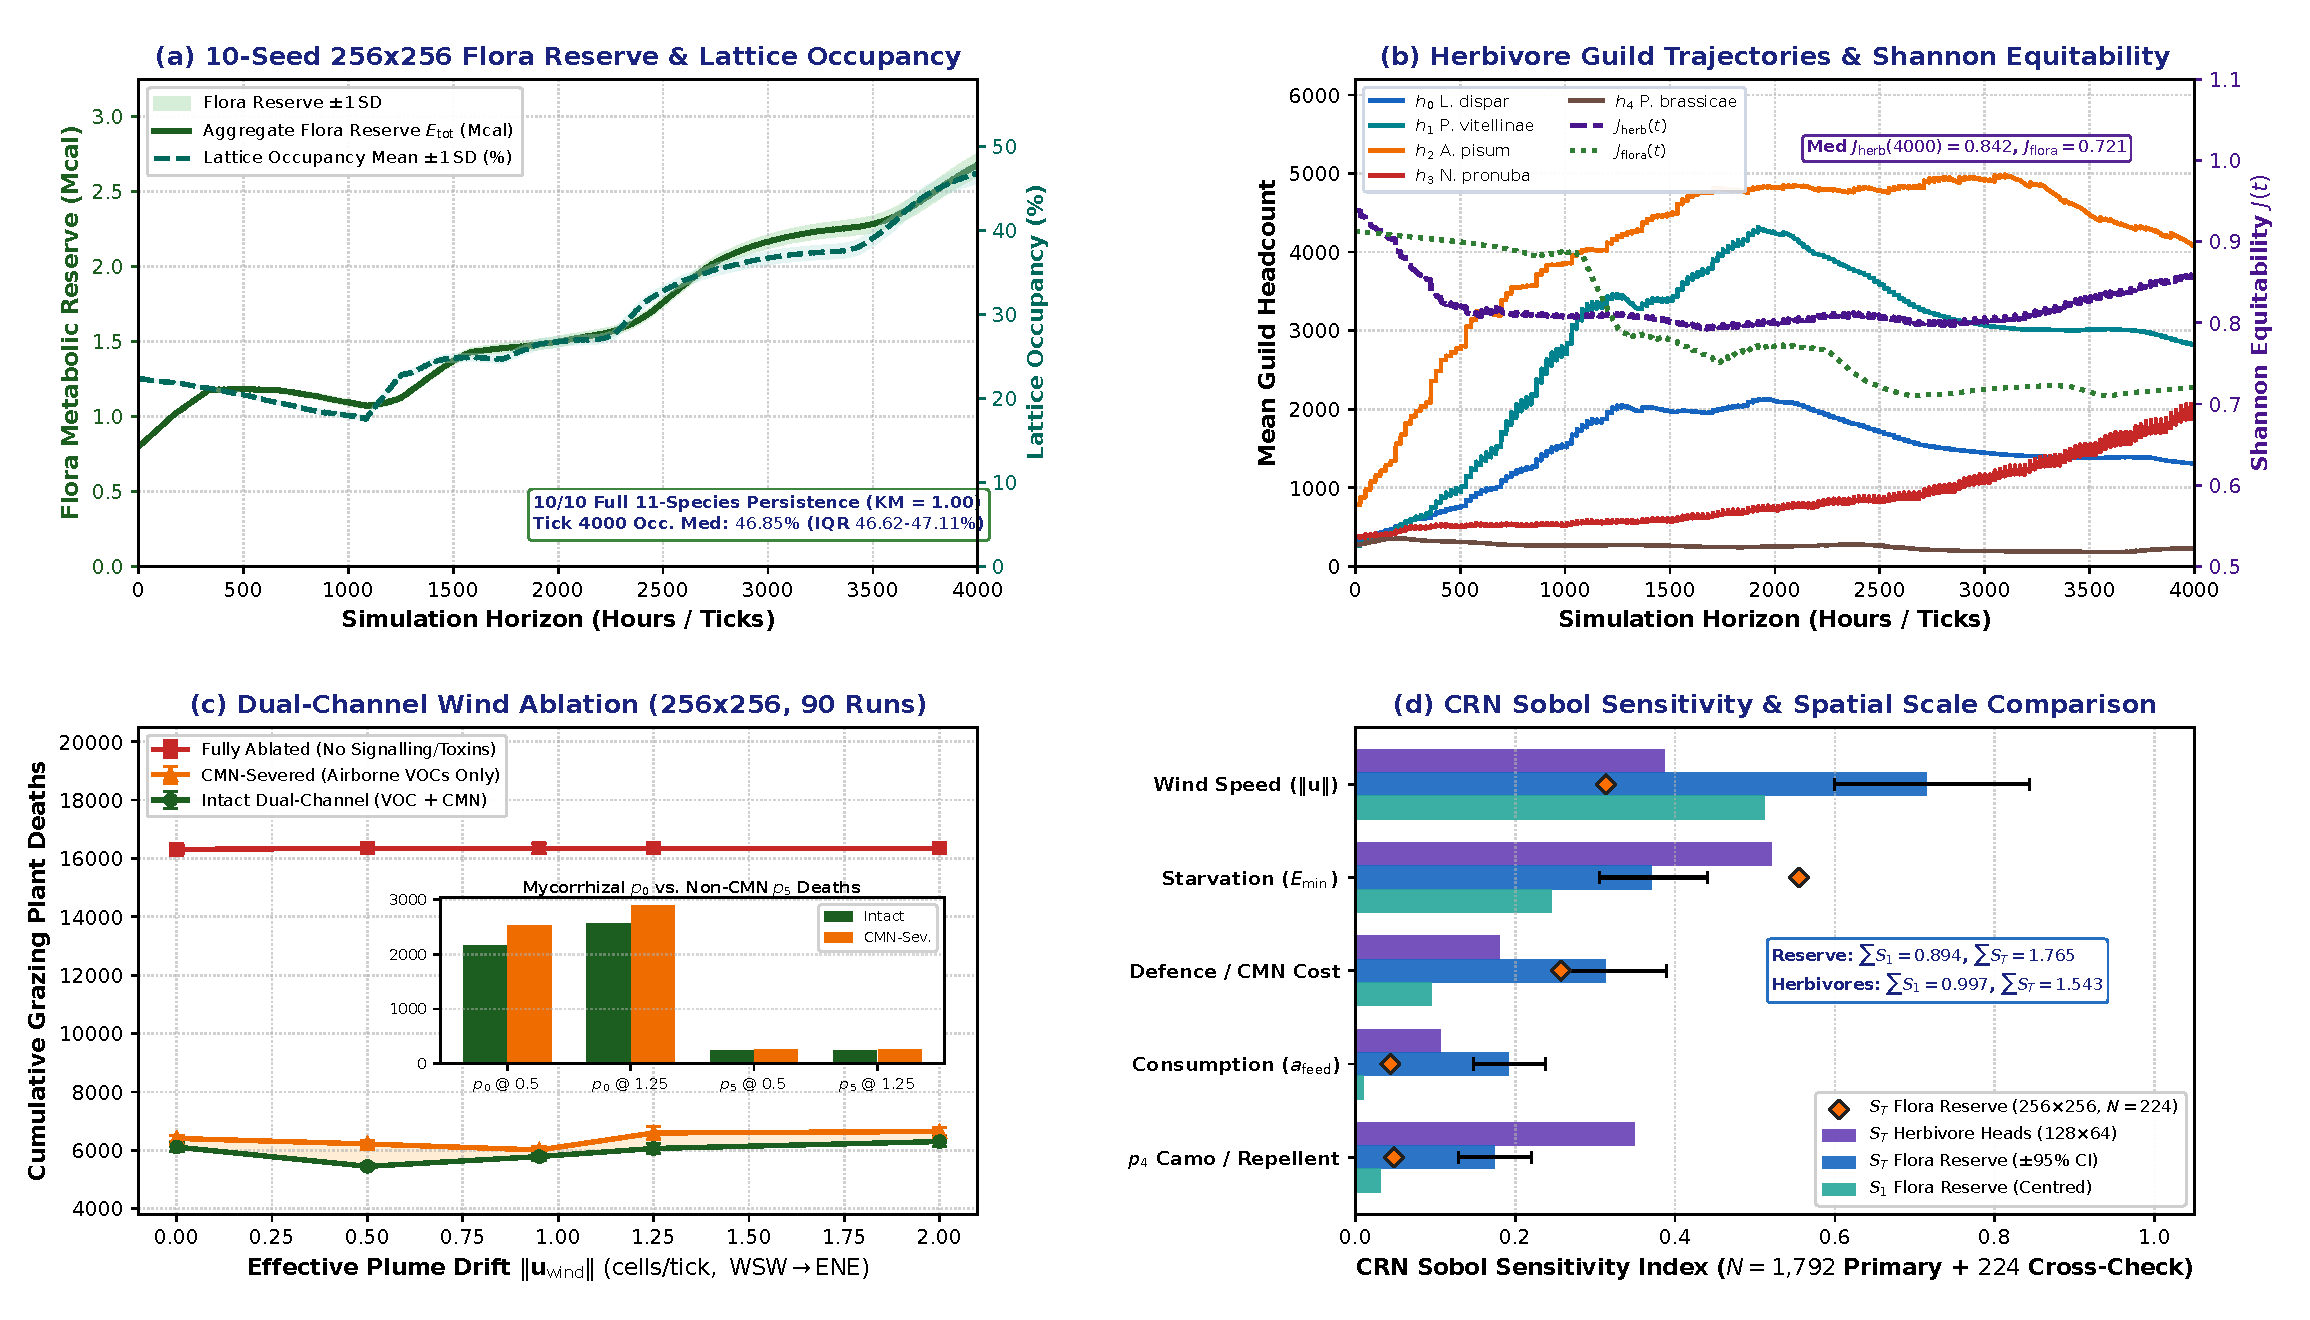
\includegraphics[width=0.92\textwidth]{figures/fig07_multispecies_coexistence.pdf}

  \caption{Empirical Multi-Species Coexistence, Dual-Channel Wind Ablation, and Variance-Based CRN Sobol Sensitivity Analysis on the Central European Ecotone. (a) Ten-seed $256 \times 256$ aggregate flora metabolic reserve ($\text{mean} \pm 1\,\text{SD}$ ribbon, Mcal) and lattice occupancy ($\%$) over $4{,}000$ ticks, reaching $46.85\%$ median terminal occupancy ($Q_{25}\text{--}Q_{75} = 46.62\%\text{--}47.11\%$). (b) Mean herbivore guild trajectories ($h_0$--$h_4$) alongside Shannon--Wiener equitability $J_{\mathrm{flora}}(t)$ and $J_{\mathrm{herb}}(t)$, confirming $10/10$ full $11$-species persistence through tick $4{,}000$. (c) Ninety-run $256 \times 256$ wind and dual-channel ablation across effective plume drift $\|\mathbf{u}_{\mathrm{wind}}\| \in [0.0, 2.0]\,\text{cells/tick}$, contrasting intact, CMN-severed, and fully ablated grazing mortality alongside the mycorrhizal ($p_0$) versus non-mycorrhizal ($p_5$) channel penalty. (d) Converged $128 \times 64$ CRN Sobol sensitivity indices ($N = 1{,}792$ runs, centred Saltelli $S_1$ and Jansen $S_T$ with $95\%$ bootstrap CIs) paired with exploratory $256 \times 256$ cross-check markers ($N = 224$ runs).}
  \label{fig:multispecies_coexistence}
\end{figure*}

Executing a $10$-seed $\times$ $4{,}000$-tick Monte Carlo ensemble (seeds $0\text{--}9$; $1{,}021.7\,\text{s}$ wall-clock across $10$ concurrent workers) evaluates zero-shot spatial scale transfer ($128 \times 64 \to 256 \times 256$) and out-of-sample single-season ($166.7$-day) persistence without retuning (Fig.~\ref{fig:multispecies_coexistence}a--b, Table~\ref{tab:ecotone_ensemble_summary}). Every flora species ($6/6$), every herbivore guild ($5/5$), and joint $11$-species coexistence maintain Kaplan--Meier persistence of $1.00$ ($10/10$ seeds) through tick $4{,}000$. Because the protocol captures one growing season rather than a multi-year stationary climax, directional successional turnover emerges cleanly: aggregate cover roughly doubles from $22.40\%$ to $46.85\%$ median terminal occupancy as cumulative riparian grazing reduces woody \textit{Populus nigra} ($p_0$, $-89\%$) and \textit{Salix purpurea} ($p_1$, $-59\%$) while fast-spreading meadow \textit{Lolium perenne} ($p_3$) expands $3.5\times$, preserving balanced community equitability and bounded oscillatory CVs throughout ticks $1{,}000\text{--}4{,}000$ (Table~\ref{tab:ecotone_ensemble_summary}, Panel~A).

All $12$ defensive pathways remain active during the final $1{,}000$-tick window on every seed, dominated by meadow CMN relays ($s_2$), \textit{Trifolium} phloem withdrawal, and CMN-primed ryegrass/clover toxins ($s_8, s_6$; Table~\ref{tab:ecotone_ensemble_summary}, Panel~B). Detailed instrumentation of \textit{Pieris brassicae} ($h_4$) on a representative trajectory verifies that the nitrile-specifier detoxification gate prevents self-poisoning: $h_4$ incurs zero self-triggered $s_7$ casualties and only $2$ collateral $s_7$ deaths across $11$ exposures (strictly when generalist $h_3$ co-occupies a $p_5$ tile), while $48/50$ toxin casualties occur on non-host meadow toxins ($s_6, s_4$). Consequently, $h_4$ lingers near its low demographic floor not through autotoxicity, but through inter-patch foraging-gap starvation ($23$ starved vs.\ $0$ toxin-killed swarms; $133$ feeding events across $497$ non-repelled daily checks) as larvae navigate the shared chemotactic field between isolated \textit{Brassica} patches ($0.70\% \to 2.80\%$ area).

\begin{table*}[b]
\caption{Ten-Seed $256 \times 256$ Calibrated Ensemble Envelopes at Tick $4{,}000$ and Late-Season ($\Delta_{3\text{k}\to 4\text{k}}$) Cascade Activations.}
\label{tab:ecotone_ensemble_summary}
\vspace{4pt}
\centering
\scriptsize
\setlength{\tabcolsep}{3.0pt}
\begin{tabular*}{\textwidth}{@{\extracolsep{\fill}} l c c @{\hspace{10pt}} l c c c @{}}
\toprule
\multicolumn{7}{@{}l}{\textbf{Panel A: Tick-$4{,}000$ Community Envelopes and Window Temporal CV ($t \in [1{,}000, 4{,}000]$, $10/10$ Full Coexistence)}} \\
\midrule
\textbf{Flora / Metric} & \textbf{Median} & \textbf{IQR ($Q_{25}\text{--}Q_{75}$)} &
\textbf{Herbivore / Metric} & \textbf{Median} & \textbf{IQR ($Q_{25}\text{--}Q_{75}$)} & \textbf{Med CV} \\
\midrule
$p_0$ \textit{Populus nigra}     & $293.0$     & $[215.3, 336.5]$     & $h_0$ \textit{Lymantria dispar}   & $1{,}220.5$ & $[1{,}097.0, 1{,}521.5]$ & $0.193$ \\
$p_1$ \textit{Salix purpurea}    & $690.0$     & $[657.0, 720.0]$     & $h_1$ \textit{Phratora vitellinae}& $2{,}801.0$ & $[2{,}683.8, 3{,}052.3]$ & $0.134$ \\
$p_2$ \textit{Trifolium repens}  & $7{,}351.0$ & $[7{,}054.3, 7{,}508.3]$ & $h_2$ \textit{Acyrthosiphon pisum}& $3{,}861.5$ & $[3{,}687.0, 4{,}681.8]$ & $0.090$ \\
$p_3$ \textit{Lolium perenne}    & $15{,}214.5$& $[15{,}025.3, 15{,}270.3]$& $h_3$ \textit{Noctua pronuba}     & $2{,}061.0$ & $[1{,}600.3, 2{,}249.0]$ & $0.430$ \\
$p_4$ \textit{Tanacetum vulgare} & $5{,}304.0$ & $[5{,}268.8, 5{,}320.0]$ & $h_4$ \textit{Pieris brassicae}   & $142.5$     & $[116.5, 264.8]$         & $0.312$ \\
$p_5$ \textit{Brassica nigra}    & $1{,}831.5$ & $[1{,}806.8, 1{,}844.8]$ & Total Herbivore Heads             & $10{,}421.0$& $[10{,}249.8, 11{,}102.8]$& $---$   \\
Occ.\ ($\%$) / $J_{\text{flora}}$& $46.85$ / $0.7207$ & $[46.62, 47.11]$ / $[0.7165, 0.7241]$ & $J_{\text{herb}}(4000)$ & $0.8418$ & $[0.8324, 0.8512]$ & $---$ \\
\bottomrule
\end{tabular*}

\vspace{3pt}
\begin{tabular*}{\textwidth}{@{\extracolsep{\fill}} l c c @{\hspace{8pt}} l c c @{\hspace{8pt}} l c c @{}}
\toprule
\multicolumn{9}{@{}l}{\textbf{Panel B: Late-Season ($\Delta_{3\text{k}\to 4\text{k}}$) Signalling, Toxin, and Phloem-Withdrawal Activations ($12/12$ Active on $10/10$ Seeds)}} \\
\midrule
\textbf{Channel} & \textbf{Med} & \textbf{IQR} & \textbf{Channel} & \textbf{Med} & \textbf{IQR} & \textbf{Channel} & \textbf{Med} & \textbf{IQR} \\
\midrule
$s_0$ GLV     & $613.0$ & $[522.0, 675.8]$ & $s_4$ Kunitz/Sal.& $354.0$     & $[299.5, 493.0]$   & $s_8$ PPO/Silica & $2{,}092.5$ & $[1{,}690.0, 2{,}423.8]$ \\
$s_1$ Ocimene & $531.0$ & $[455.0, 754.3]$ & $s_5$ Thujone    & $778.0$     & $[694.8, 881.3]$   & Phloem $p_0$     & $269.0$     & $[192.3, 680.5]$ \\
$s_2$ CMN/MeSA& $5{,}901.0$& $[5{,}146.5, 6{,}631.0]$ & $s_6$ HCN & $1{,}435.5$ & $[1{,}273.3, 1{,}718.0]$ & Phloem $p_1$ & $626.0$ & $[574.3, 964.8]$ \\
$s_3$ Benz.\ Cy.& $117.0$ & $[43.3, 238.5]$ & $s_7$ AITC ($h_3$)& $104.0$    & $[57.5, 182.5]$    & Phloem $p_2$     & $5{,}361.0$ & $[3{,}518.8, 7{,}012.3]$ \\
\bottomrule
\end{tabular*}
\end{table*}

% ==============================================================================
\subsection{Diagnostic Evaluation of Analytical Bounds (Propositions~\ref{thm:critical_synthesis_delay} and~\ref{thm:hopf_limit_cycle})}
\label{sec:ecotone_theorem_parity}
% ==============================================================================

We evaluate Propositions~\ref{thm:critical_synthesis_delay} (\eqref{eq:theta_crit_exact}) and~\ref{thm:hopf_limit_cycle} (\eqref{eq:tau_star_exact}) under the runtime Holling Type~II law~\eqref{eq:math_holling_type_ii} across single-cell continuous-grazing sweeps and all $10$ compatible host--herbivore pairs of the calibrated ecotone (Table~\ref{tab:ecotone_theorem_parity}). To project discrete parameters onto the continuous mean-field DDE in Proposition~\ref{thm:hopf_limit_cycle}, effective surrogates map directly from Table~\ref{tab:case_study_configurations} via:
\begin{align}
  a_{\text{eff}, h} &= \frac{a_h}{\max(1, v_h)}, & r_p^{\text{cont}} &= \frac{r_p}{100} \cdot \frac{E_{\mathrm{base}}}{K}, \nonumber \\
  e_{\text{eff}}^{\text{net}} &= \mathrm{clip}\!\left((1 - \delta_m)\,e_{\text{eff}},\, 0,\, 1\right), & m_{\text{herb}} &= E_{\min}^{\text{herb}} \cdot U,
  \label{eq:dde_discrete_conversion}
\end{align}
with $K = E_{\max}$ and $T_h^{\mathrm{stride}}$ taken directly from Panel~B.

Under worst-case continuous hourly grazing ($\Delta t = 1\,\text{h}$, $v = 1$, evaluating Eq.~\eqref{eq:math_holling_type_ii} every tick rather than every $24$ ticks), all single-cell sweeps confirm the closed-form critical boundary $\theta_{\text{crit}}$ cleanly: every latency strictly below $\theta_{\text{crit}}$ preserves foliar survival until toxin deployment, whereas delays above $\theta_{\text{crit}}$ collapse to $E_{\min}$ on the exact predicted tick (Table~\ref{tab:ecotone_theorem_parity}, Panel~A). At outbreak density $N_0 = 16$ (Panel~B), continuous hourly grazing yields $\theta_{\text{crit}} \in [0.3229, 1.1185]\,\text{h}$, breaching every unprimed delay and $9/10$ primed configurations (only \textit{Tanacetum} $\times$ \textit{Noctua} satisfies $\theta_{\mathrm{p}} = 1 < 1.0349\,\text{h}$). Simultaneously, isolated single-tile DDE projections yield unviable caloric fixed points ($E^* \in [0.0081, 0.0713]\,\text{cal} \ll E_{\min}$) and positive leading eigenvalues ($\alpha > 0$) even at $\tau = 0$. Consequently, full-lattice $10/10$ coexistence does not rest on local ODE equilibrium stability, instead emerging from $24$-tick diurnal feeding strides, spatial dispersal, and repellent eviction.

\begin{table*}[b]
\caption{Analytical Bound Verification (Panel~A: Continuous $1\,\mathrm{h}$ Single-Cell Grazing, $v{=}1$) and Outbreak Calibration Diagnostics (Panel~B: $N_0{=}16$ Critical Delay and Lumped DDE Projection via Eq.~\eqref{eq:dde_discrete_conversion}; Unviable $E^* \ll E_{\min}$, $\alpha > 0$ at $\tau{=}0$).}
\label{tab:ecotone_theorem_parity}
\vspace{4pt}
\centering
\scriptsize
\setlength{\tabcolsep}{3.0pt}
\begin{tabularx}{\textwidth}{
  >{\raggedright\hsize=1.00\hsize}X
  >{\centering\hsize=0.55\hsize}X
  >{\centering\hsize=0.70\hsize}X
  >{\raggedright\hsize=1.40\hsize}X
  >{\raggedright\arraybackslash\hsize=1.35\hsize}X
}
\toprule
\multicolumn{5}{@{}l}{\textbf{Panel A: Single-Cell Continuous-Grazing Verification of Proposition~\ref{thm:critical_synthesis_delay} (Eq.~\eqref{eq:theta_crit_exact})}} \\
\midrule
\textbf{Single-Cell Harness ($N_0$)} & \textbf{$\theta_{\text{crit}}$ ($\mathrm{h}$)} & \textbf{Test $\theta$} & \textbf{Surviving ($\theta < \theta_{\text{crit}}$) Outcome} & \textbf{Lethal ($\theta > \theta_{\text{crit}}$) Outcome} \\
\midrule
Reference Baseline ($N_0 = 2$) & $1.5530$ & $\{1, 2, 3, 4\}$ & $\theta = 1$: survives at $10.53\,\mathrm{cal}$ (culled tick $0$) & $\theta \in \{2, 3, 4\}$: plant dies tick $1$ \\
Ecotone $p_3 \times h_3$ ($N_0 = 5$) & $3.5791$ & $\{2, 3, 4, 10\}$ & $\theta \in \{2, 3\}$: survive at $28.41$ / $16.03\,\mathrm{cal}$ & $\theta \in \{4, 10\}$: plant dies tick $3$ \\
Ecotone $p_0 \times h_0$ ($N_0 = 4$) & $1.8372$ & $\{1, 2, 3, 12\}$ & $\theta = 1$: survives at $37.36\,\mathrm{cal}$ (culled tick $0$) & $\theta \in \{2, 3, 12\}$: plant dies tick $1$ \\
\bottomrule
\end{tabularx}

\vspace{3pt}
\setlength{\tabcolsep}{2.5pt}
\begin{tabular*}{\textwidth}{@{\extracolsep{\fill}} l c c c c c c c @{}}
\toprule
\multicolumn{8}{@{}l}{\textbf{Panel B: Compatible Calibrated Ecotone Pairs Under Outbreak Continuous Grazing ($N_0 = 16$) and Zero-Delay DDE Diagnostics}} \\
\midrule
\textbf{Pair} & \textbf{$E_0 / E_{\min}$ ($\mathrm{cal}$)} & \textbf{$a_{\text{eff},h}$ ($\mathrm{str.}^{-1}$)} & \textbf{$T_h^{\mathrm{stride}}$ ($\mathrm{str.}\cdot\mathrm{cal}^{-1}$)} & \textbf{$\theta_{\text{p}} / \theta_{\text{u}}$} & \textbf{$\theta_{\text{crit}}$ ($\mathrm{h}$)} & \textbf{$E^* / N^*$ ($\mathrm{cal} / \mathrm{ind.}$)} & \textbf{$\alpha$ ($\tau = 0$)} \\
\midrule
$p_0 \times h_0$ & $70 / 14$ & $1.6668$ & $0.1140$ & $2 / 12$ & $0.4593$ & $0.0213 / 0.0005$ & $+3.0{\times}10^{-6}$ \\
$p_1 \times h_0$ & $60 / 12$ & $1.6668$ & $0.1140$ & $2 / 12$ & $0.4023$ & $0.0302 / 0.0003$ & $+3.0{\times}10^{-6}$ \\
$p_0 \times h_1$ & $70 / 14$ & $1.1761$ & $0.1726$ & $2 / 12$ & $0.6896$ & $0.0229 / 0.0006$ & $+3.0{\times}10^{-6}$ \\
$p_1 \times h_1$ & $60 / 12$ & $1.1761$ & $0.1726$ & $2 / 12$ & $0.6033$ & $0.0326 / 0.0004$ & $+3.0{\times}10^{-6}$ \\
$p_2 \times h_2$ & $45 / 9$  & $2.6664$ & $0.1268$ & $1 / 8$  & $0.3229$ & $0.0081 / 0.0006$ & $+4.0{\times}10^{-6}$ \\
$p_2 \times h_3$ & $45 / 9$  & $0.5046$ & $0.3342$ & $1 / 8$  & $0.9514$ & $0.0503 / 0.0032$ & $+1.2{\times}10^{-5}$ \\
$p_3 \times h_3$ & $55 / 11$ & $0.5046$ & $0.3342$ & $2 / 10$ & $1.1185$ & $0.0713 / 0.0034$ & $+1.9{\times}10^{-5}$ \\
$p_4 \times h_3$ & $50 / 10$ & $0.5046$ & $0.3342$ & $1 / 3$  & $1.0349$ & $0.0562 / 0.0018$ & $+8.0{\times}10^{-6}$ \\
$p_5 \times h_3$ & $35 / 7$  & $0.5046$ & $0.3342$ & $2 / 8$  & $0.7842$ & $0.0498 / 0.0053$ & $+2.0{\times}10^{-5}$ \\
$p_5 \times h_4$ & $35 / 7$  & $1.3532$ & $0.1633$ & $2 / 8$  & $0.3601$ & $0.0171 / 0.0020$ & $+9.0{\times}10^{-6}$ \\
\bottomrule
\end{tabular*}
\end{table*}

% ==============================================================================
\subsection{Dual-Channel Wind Ablation and Upwind CMN Crossover}
\label{sec:ecotone_ablation}
% ==============================================================================

To separate airborne VOC plumes from subterranean root-link conduits across shifting drift regimes, we executed a $90$-run factorial ablation on the $256 \times 256$ ecotone ($6$ seeds $\times$ $5$ wind speeds $\|\mathbf{u}_{\text{wind}}\| \in [0.0, 2.0]\,\text{cells/tick}$ along WSW$\to$ENE $\times$ $3$ treatments: intact, CMN-severed, and fully ablated; $2{,}500$ ticks; Table~\ref{tab:ecotone_ablation} and Fig.~\ref{fig:multispecies_coexistence}c), paired with a $21$-run deterministic $20$-tick upwind relay test on a $64 \times 64$ seven-plant cardinal chain.

First, removing all signalling and inducible toxins (fully ablated) raises cumulative grazing deaths $2.6\times\text{--}3.0\times$, more than doubles late-horizon herbivore headcounts, and cuts tail flora reserves by roughly $40\%$ (Table~\ref{tab:ecotone_ablation}). Because cleared trigger rules keep every volatile field strictly zero, wind magnitude leaves chemical transport unchanged once signalling is off; seed raycasting uses isotropic sampling under calm air and the normalised unit direction $\mathbf{u}$ along $22.5^\circ$ (Eqs.~\eqref{eq:seed_projection_x}--\eqref{eq:seed_projection_y}) for every positive drift speed, rendering all four positive-drift fully ablated conditions bit-identical on shared seeds (collapsed into the bottom row of Table~\ref{tab:ecotone_ablation}).

Second, severing subterranean CMNs while preserving airborne VOCs increases total grazing mortality across every tested wind speed, peaking at $+14.1\%$ under half-cell drift ($\|\mathbf{u}_{\text{wind}}\| = 0.50\,\text{cells/tick}$, Wilcoxon $p = 0.0312$). Intact grazing deaths attain their global minimum at $0.50\,\text{cells/tick}$, matching the theoretical peak in implicit bilinear numerical diffusion ($\sigma_{\text{num}}^2 = 0.25$, Section~\ref{subsec:operator_splitting}) that widens lateral VOC pre-warming. Disaggregating by guild isolates the statistically consistent CMN-severing penalty squarely on woody mycorrhizal \textit{Populus} ($p_0$, $+10.7\%$ to $+16.7\%$, $p = 0.0312$ across all positive drift speeds), whereas fast-recovering meadow guilds ($p_2 + p_3$) exhibit larger inter-seed variance and the embedded non-mycorrhizal control \textit{Brassica nigra} ($p_5$) displays zero statistically significant sensitivity ($p \ge 0.1562$), confirming specificity to connected root networks. Under the deterministic $20$-tick cardinal relay chain, calm air ($u_x = 0.0$) primes all three upwind and downwind hops symmetrically within ticks $1\text{--}3$. Once $u_x \ge 0.95\,\text{cells/tick}$, airborne-only transport fails completely upwind ($0/3$ hops), whereas intact CMN conduits ($6$ links, $g_{\mathrm{relay}} = 2$) preserve all $3$ upwind priming hops across $u_x \in \{0.95, 1.00, 1.08\}\,\text{cells/tick}$ and $1$ upwind hop at $1.25\,\text{cells/tick}$ before advective washout at $2.00\,\text{cells/tick}$.

\begin{table*}[b]
\caption{Ninety-Run $256 \times 256$ Dual-Channel Wind Ablation Summary ($n=6$ Seeds per Cell, $2{,}500$ Ticks, Mean $\pm$ SE; Paired Wilcoxon $p$ Comparing CMN-Severed vs.\ Intact).}
\label{tab:ecotone_ablation}
\vspace{4pt}
\centering
\scriptsize
\setlength{\tabcolsep}{1.2pt}
\begin{tabular*}{\textwidth}{@{\extracolsep{\fill}} c l c c c c c c c c @{}}
\toprule
\textbf{$\|\mathbf{u}\|$} & \textbf{Treatment} & \textbf{Total $\pm$ SE} & \textbf{Heads} & \textbf{Tail} & \textbf{$J_{\text{f}}$} & \textbf{$J_{\text{h}}$} & \textbf{$p_0 \pm$ SE ($p$)} & \textbf{$p_2{+}p_3 \pm$ SE ($p$)} & \textbf{$p_5 \pm$ SE ($p$)} \\
\midrule
$0.00$ & Intact         & $6{,}108{\pm}146$ & $12{,}728$ & $1.53$ & $.741$ & $.823$ & $2{,}605{\pm}31$ & $1{,}802{\pm}121$ & $231{\pm}9$ \\
$0.00$ & CMN-Sev.       & $6{,}404{\pm}107^{\ast}$ & $13{,}789$ & $1.53$ & $.730$ & $.809$ & $2{,}841{\pm}48$ ($.063$) & $1{,}810{\pm}133$ ($.688$) & $226{\pm}7$ ($.313$) \\
$0.00$ & Ablated        & $16{,}310{\pm}123$& $26{,}952$ & $0.90$ & $.825$ & $.718$ & $3{,}099{\pm}71$ & $10{,}897{\pm}54$ & $581{\pm}18$ \\
\midrule
$0.50$ & Intact         & $5{,}447{\pm}86$  & $11{,}297$ & $1.50$ & $.734$ & $.825$ & $2{,}168{\pm}36$ & $1{,}692{\pm}91$  & $231{\pm}13$ \\
$0.50$ & CMN-Sev.       & $6{,}214{\pm}117^{\ast}$ & $13{,}089$ & $1.50$ & $.728$ & $.827$ & $2{,}529{\pm}33^{\ast}$ ($.031$) & $1{,}994{\pm}108$ ($.063$) & $261{\pm}17$ ($.406$) \\
$0.95$ & Intact         & $5{,}783{\pm}117$ & $11{,}910$ & $1.46$ & $.718$ & $.786$ & $2{,}332{\pm}23$ & $1{,}876{\pm}116$ & $254{\pm}9$ \\
$0.95$ & CMN-Sev.       & $6{,}008{\pm}120$ & $12{,}264$ & $1.48$ & $.710$ & $.831$ & $2{,}644{\pm}36^{\ast}$ ($.031$) & $1{,}721{\pm}105$ ($.313$) & $231{\pm}12$ ($.156$) \\
$1.25$ & Intact         & $6{,}059{\pm}186$ & $12{,}657$ & $1.44$ & $.719$ & $.789$ & $2{,}565{\pm}31$ & $1{,}960{\pm}168$ & $233{\pm}21$ \\
$1.25$ & CMN-Sev.       & $6{,}590{\pm}219$ & $13{,}255$ & $1.47$ & $.711$ & $.817$ & $2{,}893{\pm}28^{\ast}$ ($.031$) & $2{,}028{\pm}191$ ($.688$) & $256{\pm}11$ ($.438$) \\
$2.00$ & Intact         & $6{,}297{\pm}156$ & $13{,}631$ & $1.43$ & $.716$ & $.809$ & $2{,}672{\pm}15$ & $2{,}097{\pm}144$ & $243{\pm}12$ \\
$2.00$ & CMN-Sev.       & $6{,}642{\pm}129$ & $13{,}946$ & $1.46$ & $.708$ & $.817$ & $2{,}957{\pm}44^{\ast}$ ($.031$) & $1{,}994{\pm}140$ ($.313$) & $258{\pm}15$ ($.313$) \\
\midrule
$>0.00^{\dagger}$ & Ablated & $16{,}351{\pm}178$& $27{,}211$ & $0.87$ & $.812$ & $.725$ & $3{,}217{\pm}74$ & $10{,}856{\pm}164$ & $590{\pm}10$ \\
\bottomrule
\multicolumn{10}{@{}p{\textwidth}@{}}{$^{\ast}$Two-sided paired Wilcoxon $p = 0.0312 < 0.05$ ($W = 0.0, n = 6$). Units: $\|\mathbf{u}\|$ ($\mathrm{cells/tick}$), Tail ($\mathrm{Mcal}$). $^{\dagger}$Bit-identical across $\|\mathbf{u}_{\text{wind}}\| \in \{0.50, 0.95, 1.25, 2.00\}\,\mathrm{cells/tick}$ along $22.5^\circ$: inactive chemical triggers leave seed raycasting dependent solely on normalised direction $\mathbf{u}$ (Eqs.~\eqref{eq:seed_projection_x}--\eqref{eq:seed_projection_y}).}
\end{tabular*}
\end{table*}

% ==============================================================================
\subsection{Variance-Based Global Sensitivity Analysis (CRN Sobol GSA)}
\label{sec:ecotone_sobol}
% ==============================================================================

To partition output variance into direct main effects and multi-factor interactions, we apply variance-based Sobol Global Sensitivity Analysis \cite{saltelli2010variance} using a scrambled quasi-random Sobol sequence implemented in SciPy \cite{virtanen2020scipy}. For a scalar output $Y = f(\mathbf{X})$ over $k$ independent inputs $\mathbf{X} = (X_1, \dots, X_k)$, the orthogonal Hoeffding--Sobol decomposition defines first-order ($S_i$) and total-order ($S_{T_i}$) indices:
\begin{align}
  S_i &= \frac{V_{X_i}\!\left(\mathbb{E}_{\mathbf{X}_{\sim i}}[Y \mid X_i]\right)}{V(Y)}, \nonumber \\
  S_{T_i} &= \frac{\mathbb{E}_{\mathbf{X}_{\sim i}}\!\left[V_{X_i}(Y \mid \mathbf{X}_{\sim i})\right]}{V(Y)} = 1 - \frac{V_{\mathbf{X}_{\sim i}}\!\left(\mathbb{E}_{X_i}[Y \mid \mathbf{X}_{\sim i}]\right)}{V(Y)},
  \label{eq:sobol_def}
\end{align}
evaluated via a Saltelli radial design ($N = n_{\text{base}}(k + 2)$ runs) over sample matrices $\mathbf{A}, \mathbf{B} \in \mathbb{R}^{n_{\text{base}} \times k}$ and hybrid blocks $\mathbf{A}_{\mathbf{B}}^{(i)}$ \cite{saltelli2010variance}. Holding the stochastic seed fixed across every design row (Common Random Numbers, CRN) eliminates between-seed Monte Carlo variance. Because mean flora reserve exhibits a high mean-to-standard-deviation ratio ($\mu / \sigma \approx 11.9$), subtracting the pooled baseline mean $\bar{y}$ of $\mathbf{A} \cup \mathbf{B}$ alongside the Jansen estimator \cite{jansen1999analysis} stabilises finite-sample estimation:
\begin{align}
  \hat{S}_i &= \frac{\frac{1}{n_{\mathrm{base}}}\sum_{j=1}^{n_{\mathrm{base}}} \left(y_{\mathbf{B},j} - \bar{y}\right)\left(y_{\mathbf{A}_{\mathbf{B}}^{(i)},j} - y_{\mathbf{A},j}\right)}{\widehat{V}_{\mathbf{A}\cup\mathbf{B}}(Y)}, \nonumber \\
  \hat{S}_{T_i} &= \frac{\frac{1}{2\,n_{\mathrm{base}}}\sum_{j=1}^{n_{\mathrm{base}}} \left(y_{\mathbf{A},j} - y_{\mathbf{A}_{\mathbf{B}}^{(i)},j}\right)^2}{\widehat{V}_{\mathbf{A}\cup\mathbf{B}}(Y)},
  \label{eq:sobol_estimators}
\end{align}
using unbiased sample variance over $\mathbf{A} \cup \mathbf{B}$ and $500$ bootstrap resamples for $95\%$ confidence intervals.

We jointly sampled $k = 5$ biophysical multipliers across per-stride consumption rate ($\kappa_a$), herbivore starvation threshold ($\kappa_{E_{\min}}$), combined defence and CMN upkeep ($\kappa_{\mathrm{cost}}$), effective plume drift ($\|\mathbf{u}_{\text{wind}}\|$), and $p_4$ olfactory strength ($s_{p_4}$, setting $\Phi_{\text{camo}} = 1 - 0.75 s_{p_4}$ and $s_5$ eviction duration $\max(1, \mathrm{round}(8 s_{p_4}))$). The primary $128 \times 64$ GSA executed $n_{\text{base}} = 256$ ($N = 1{,}792$ runs, $1{,}500$ ticks, $6{,}991.5\,\text{s}$), paired with an exploratory $256 \times 256$ cross-check ($n_{\text{base}} = 32$, $N = 224$ runs, $1{,}000$ ticks, $3{,}712.7\,\text{s}$).

Across all $15$ factor--output pairs of the converged $128 \times 64$ suite (Table~\ref{tab:ecotone_sobol}, Fig.~\ref{fig:multispecies_coexistence}d), $S_1 \le S_T$ holds strictly throughout with total-order indices summing cleanly to $\sum S_T \in [1.543, 1.938]$ ($\sum S_1 \in [0.838, 0.997]$; the lone small negative Saltelli estimate $S_1 = -0.042$ for $\kappa_{\mathrm{cost}}$ on $J_{\text{flora}}$ reflects finite-sample estimator noise around a near-zero main effect). Plume drift $\|\mathbf{u}_{\text{wind}}\|$ dominates both aggregate vegetation reserve and terminal flora equitability, whereas the herbivore starvation threshold $\kappa_{E_{\min}}$ governs terminal herbivore headcounts; $p_4$ olfactory shielding and defence/CMN costs contribute predominantly through multi-factor interactions ($S_T \gg S_1$). In addition, consumption-rate scaling $\kappa_a$ exhibits negligible direct main effects ($S_1 \le 0.027$) across all outputs and both lattice scales, confirming the kinetic mechanism in Eq.~\eqref{eq:math_holling_type_ii}: because diurnal calibrated parameters operate near the Holling Type~II saturation ceiling $1/T_h^{\mathrm{stride}}$ ($a_{\mathrm{eff}} T_h^{\mathrm{stride}} E \approx 9.3 \gg 1$ on meadow clover and ryegrass), perturbations in attack rate minimally alter per-event intake compared against advective plume geometry and metabolic starvation thresholds. Despite finite-sample Saltelli noise at $n_{\text{base}} = 32$ ($S_1 \in [-0.111, +0.593]$, one sample exceedance $S_1 = +0.268 > S_T$ for $\kappa_{\mathrm{cost}}$ on reserve), the $256 \times 256$ cross-check preserves the identical dominance hierarchy ($\kappa_{E_{\min}}$ and $\|\mathbf{u}_{\text{wind}}\|$ leading; $\kappa_a$ negligible).

\begin{table*}[b]
\caption{CRN Sobol Sensitivity Indices: Primary Converged $128 \times 64$ Design ($n_{\mathrm{base}}{=}256$, $N{=}1{,}792$, $1{,}500$ Ticks; $S_1$ Centred Saltelli and $S_T$ Jansen with $95\%$ Bootstrap CIs) Alongside Exploratory $256 \times 256$ Cross-Check ($n_{\mathrm{base}}{=}32$, $N{=}224$, $1{,}000$ Ticks).}
\label{tab:ecotone_sobol}
\vspace{4pt}
\centering
\scriptsize
\setlength{\tabcolsep}{1.8pt}
\begin{tabular*}{\textwidth}{@{\extracolsep{\fill}} l c c c @{\hspace{6pt}} c c c @{\hspace{6pt}} c c c @{}}
\toprule
\textbf{Factor (Range)} &
\multicolumn{3}{c}{\textbf{Mean Flora Reserve}} &
\multicolumn{3}{c}{\textbf{Terminal $J_{\text{flora}}$}} &
\multicolumn{3}{c}{\textbf{Terminal Herbivore Heads}} \\
\cmidrule(lr){2-4} \cmidrule(lr){5-7} \cmidrule(lr){8-10}
& \textbf{$S_1$} & \textbf{$S_T$ [$95\%$ CI]} & \textbf{$S_T^{(256)}$} &
  \textbf{$S_1$} & \textbf{$S_T$ [$95\%$ CI]} & \textbf{$S_T^{(256)}$} &
  \textbf{$S_1$} & \textbf{$S_T$ [$95\%$ CI]} & \textbf{$S_T^{(256)}$} \\
\midrule
Intake $\kappa_a$ ($[0.8, 1.4]$) &
$+0.011$ & $0.192\,[0.148, 0.238]$ & $0.044$ &
$+0.027$ & $0.264\,[0.213, 0.326]$ & $0.128$ &
$+0.005$ & $0.106\,[0.087, 0.132]$ & $0.033$ \\
Starv.\ $\kappa_{E_{\min}}$ ($[0.7, 1.3]$) &
$+0.245$ & $0.371\,[0.305, 0.441]$ & $0.555$ &
$+0.223$ & $0.403\,[0.331, 0.483]$ & $0.502$ &
$+0.440$ & $0.521\,[0.437, 0.614]$ & $0.674$ \\
Cost $\kappa_{\mathrm{cost}}$ ($[0.5, 1.5]$) &
$+0.095$ & $0.313\,[0.253, 0.390]$ & $0.257$ &
$-0.042$ & $0.245\,[0.198, 0.299]$ & $0.171$ &
$+0.088$ & $0.180\,[0.141, 0.233]$ & $0.098$ \\
Drift $\|\mathbf{u}_{\text{wind}}\|$ ($[0, 2]\,\mathrm{c/t}$) &
$+0.512$ & $0.715\,[0.599, 0.844]$ & $0.314$ &
$+0.567$ & $0.731\,[0.624, 0.856]$ & $0.561$ &
$+0.259$ & $0.387\,[0.315, 0.464]$ & $0.176$ \\
Camo $s_{p_4}$ ($[0.2, 1.0]$) &
$+0.031$ & $0.174\,[0.129, 0.220]$ & $0.048$ &
$+0.063$ & $0.296\,[0.235, 0.369]$ & $0.109$ &
$+0.206$ & $0.349\,[0.283, 0.429]$ & $0.063$ \\
\midrule
\textbf{Index Sums ($\sum S_1 / \sum S_T$)} &
$0.894$ & $1.765$ & $1.218$ &
$0.838$ & $1.938$ & $1.470$ &
$0.997$ & $1.543$ & $1.044$ \\
\bottomrule
\multicolumn{10}{@{}p{\textwidth}@{}}{$128 \times 64$ output distributions (mean $\pm$ SD): flora reserve $145{,}228 \pm 12{,}240\,\mathrm{cal}$, $J_{\text{flora}} = 0.768 \pm 0.052$, herbivore heads $2{,}200.5 \pm 742.8$. Exploratory $256 \times 256$ distributions: reserve $1{,}150{,}485 \pm 51{,}017\,\mathrm{cal}$, $J_{\text{flora}} = 0.884 \pm 0.015$, heads $10{,}530.2 \pm 2{,}994.4$. Units: $\mathrm{c/t} \equiv \mathrm{cells/tick}$.}
\end{tabular*}
\end{table*}


% ==============================================================================
% Section 7: Computational Realisation & Execution Engine
% ==============================================================================
% ==============================================================================
% Section 7: Computational Realisation & Execution Engine
% ==============================================================================

\section{Computational Realisation and Execution Engine}
\label{sec:computational_realisation}

Coupled hybrid simulations combining thousands of mobile agents with continuous reaction--diffusion--advection PDEs incur severe interpreter and allocation overhead in pointer-based frameworks. To eliminate dynamic heap jitter and cache thrashing, PHIDS employs a data-oriented Entity--Component--System (ECS) whose PDE stencils, flow-field relaxation, and spatial indexing loops compile to native machine code via Just-In-Time (JIT) compilation on an Intel Core i7-10750H testbed ($6$ cores, $12$ threads, $2.60\,\text{GHz}$ base clock, AVX2/FMA, $192\,\text{KiB}$ L1d, $192\,\text{KiB}$ L1i, $1.5\,\text{MiB}$ L2, $12\,\text{MiB}$ shared L3, $31\,\text{GiB}$ RAM) running Linux~6.18.64, Python~3.13.12, NumPy~2.5.3 \cite{harris2020array}, and Numba~0.67.0 (LLVM~22.1.0) \cite{lam2015numba}. Table~\ref{tab:hardware_execution_benchmarks} gathers measured internal kernel ablations, lattice scaling, OpenMP threading, and per-stage profiling; below we detail the array layout, zero-allocation compilation, scaling bottlenecks, thread determinism, and compressed replay storage.

% ==============================================================================
% Table 9 (LaTeX tab08): Internal PHIDS Kernel Ablations & Hardware Benchmarks
% ==============================================================================

\begin{table*}[t]
\caption{Internal Engine Ablations, Grid Scaling, OpenMP Threading, and Per-Stage Tick Breakdown on the Six-Core i7-10750H Testbed.}
\label{tab:hardware_execution_benchmarks}
\vspace{4pt}
\centering
\scriptsize
\setlength{\tabcolsep}{3.0pt}
\begin{tabularx}{\textwidth}{
  >{\raggedright\hsize=0.95\hsize}X
  >{\raggedright\hsize=0.92\hsize}X
  >{\raggedright\hsize=1.28\hsize}X
  >{\centering\hsize=0.65\hsize}X
  >{\raggedright\hsize=1.08\hsize}X
  >{\raggedright\arraybackslash\hsize=1.12\hsize}X
}
\toprule
\multicolumn{6}{@{}l}{\textbf{Panel A: Internal Kernel, Storage, and Parallel Scaling Ablations}} \\
\midrule
\textbf{Engine Mechanism} & \textbf{Baseline Config.} & \textbf{Optimised PHIDS Config.} & \textbf{Complexity} & \textbf{Bottleneck / Action} & \textbf{Speedup / Outcome} \\
\midrule
Toroidal Wrapping & Modulo (\texttt{\% W}, \texttt{\% H}) & Bitwise \texttt{AND} ($W = 2^k$) & $\mathcal{O}(1)$ & Removes integer division & $\mathbf{13.0\times}$ ($1.04$ vs.\ $13.48\,\mathrm{ns/op}$) \\
Kernel JIT ($64\times 32$) & Pure Python ($p = 1$) & Numba LLVM ($p = 1$) & $\mathcal{O}(|\Lambda| + N)$ & Removes interpreter overhead & $\mathbf{138.0\times}$ ($1.13$ vs.\ $156.46\,\mathrm{ms}$) \\
Kernel JIT ($128^2$) & Pure Python ($p = 1$) & Numba LLVM ($p = 1$) & $\mathcal{O}(|\Lambda| + N)$ & Native AVX2 PDE sweeps & $\mathbf{262.0\times}$ ($2.33$ vs.\ $609.46\,\mathrm{ms}$) \\
OpenMP ($256^2$ 3-sp.) & Single thread ($68.90\,\mathrm{ms}$) & $p \in \{2,4,6,12\}$: $55.6, 50.8, 50.5, 50.5\,\mathrm{ms}$ & $\mathcal{O}((|\Lambda| + N)/p)$ & $12\,\mathrm{MiB}$ L3 / DRAM bound & $\mathbf{1.37\times}$ peak ($p = 6$) \\
Thread Determinism & Serial ($p = 1$) & OpenMP ($p \in \{1, 4, 12\}$) ping-pong & $\mathcal{O}(1)$ swap & Disjoint writes \& max order & \textbf{Bit-Exact} ($\max|\Delta| = 0.0$) \\
Replay Storage & Raw \texttt{float32} volume & Chunked Zarr + Zstd & $\mathcal{O}(|\Lambda|)$ & Zero-run sparsity ($\epsilon = 10^{-4}$) & $\mathbf{10.5\text{--}12.1\times}$ ($3.76$; $141.7\,\mathrm{MB}$) \\
\bottomrule
\end{tabularx}

\vspace{3pt}
\setlength{\tabcolsep}{1.8pt}
\begin{tabular*}{\textwidth}{@{\extracolsep{\fill}} l c c c c c c c c @{}}
\toprule
\multicolumn{9}{@{}l}{\textbf{Panel B: Coupled Grid Scaling ($p{=}12$) and Per-Stage Tick Breakdown (Mean $\mathrm{ms}$, Unreplayed Benchmarks)}} \\
\midrule
\textbf{Workload (Active Entities)} & \textbf{Med (p95)} & \textbf{Mean} & \textbf{Flow} & \textbf{Life.} & \textbf{Int.} & \textbf{Sig.} & \textbf{Diff.} & \textbf{Reb./Tel.} \\
\midrule
$64 \times 32$ Orchard ($15$ pl., $1$ sw.) & $1.25$ ($1.40$) & $---$ & $---$ & $---$ & $---$ & $---$ & $---$ & $---$ \\
$128^2$ Canopy ($7$ pl., $1$ sw., $0$ sub.) & $2.59$ ($2.91$) & $3.20$ & $1.81$ & $0.02$ & $0.07$ & $0.36$ & $0.17$ & $0.71 / 0.05$ \\
$256^2$ Sparse 3-sp.\ ($15{,}714$ pl.) & $36.62$ ($81.96$) & $---$ & $---$ & $---$ & $---$ & $---$ & $---$ & $---$ \\
$256^2$ Eq.\ 3-sp.\ ($25{,}559$ / $21{,}692$ prof.) & $57.23$ ($147.97$) & $66.36$ & $9.60$ & $19.83^{\dagger}$ & $1.48$ & $18.63$ & $3.55$ & $3.10 / 10.18$ \\
$256^2$ 11-sp.\ Ecotone (t\,$10$--$35$: $14.6\text{k}$ pl.) & $55.19$ ($120.96$) & $64.62$ & $7.64$ & $13.12^{\dagger}$ & $0.69$ & $28.56$ & $4.46$ & $2.94 / 7.20$ \\
$256^2$ 11-sp.\ Ecotone ($4{,}000$\,t; $360$\,t Zarr) & $162.55^{\ddagger}$ ($245.71^{\ddagger}$) & $137.00$ & \multicolumn{6}{@{}l}{Standalone $4{,}000$-t run: $547.9\,\mathrm{s}$ (${\sim}30.7\text{k}$ mean flora)} \\
\bottomrule
\multicolumn{9}{@{}p{\textwidth}@{}}{$^{\dagger}$Includes periodic $8$-tick mycorrhizal graph construction spikes (p95 lifecycle $77.94\,\mathrm{ms}$ on 3-sp., $57.23\,\mathrm{ms}$ on 11-sp.; medians $6.43$ / $3.67\,\mathrm{ms}$). $^{\ddagger}$Measured during active $360$-tick chunked Zstandard Zarr streaming ($162.55\,\mathrm{ms}$ median; raw tensors $39.32$ and $1{,}710.0\,\mathrm{MB}$).}
\end{tabular*}
\end{table*}


% ==============================================================================
\subsection{Data-Oriented Entity--Component--System Architecture}
\label{subsec:data_oriented_ecs}
% ==============================================================================

Instead of fragmenting state across per-entity heap objects, PHIDS stores continuous field tensors and species slices in contiguous C-order NumPy arrays --- double-precision (\texttt{float64}) for energy, volatile signals, toxins, nutrition, and chemotactic flow fields, and single-precision (\texttt{float32}) for structural mass layers \cite{harris2020array}:
\begin{align}
  \mathbf{E}_{\mathrm{flora}}, \bm{\eta}_{\mathrm{nutr}}, \mathbf{F}_{\mathrm{flow}} &\in \mathbb{R}^{W \times H}, \\
  \mathbf{C}_{\mathrm{sig}}, \mathbf{T}_{\mathrm{tox}} &\in \mathbb{R}^{16 \times W \times H}, \quad \mathbf{M}_{\mathrm{struct}} \in \mathbb{R}_{\mathrm{f32}}^{16 \times W \times H}.
\end{align}
Per-entity attributes reside in slotted containers indexed over integer entity identifiers via an $\mathcal{O}(1)$ spatial hash. To bound tensor widths and preserve predictable L1-cache footprints without runtime array resizing, PHIDS pre-allocates static leading dimension $K \le 16$ across interaction tensors: the diet matrix $\mathbf{D} \in \{0, 1\}^{16 \times 16}$ occupies a contiguous $256\,\text{bytes}$, and signal and toxin layers pre-allocate $16$ channels for $\mathcal{O}(1)$ slice indexing.

% ==============================================================================
\subsection{Zero-Allocation JIT Compilation and Branchless Masking}
\label{subsec:jit_compilation_simd}
% ==============================================================================

Spatial inner loops --- semi-Lagrangian backward interpolation, $5 \times 5$ Gaussian convolution, Jacobi potential relaxation (OpenMP-parallelised across rows for $W \cdot H \ge 128^2$ and serial on smaller grids), and chemotactic neighbour scoring --- compile to native machine code via Numba/LLVM \cite{lam2015numba}. Write buffers, advection scratch planes, and 5-cell candidate arrays are pre-allocated once at initialisation and mutated in place without inner-loop heap allocation. To allow LLVM loop vectorisation without branch divergence, threshold gating and clamping execute via arithmetic saturation and $0.0/1.0$ float masks (Eqs.~\eqref{eq:subnormal_clamping} and~\eqref{eq:capacity_mask}). Disabling JIT compilation slows execution by $138.0\times$ on the $64 \times 32$ orchard and $262.0\times$ on the $128 \times 128$ canopy (Table~\ref{tab:hardware_execution_benchmarks}, Panel~A).

% ==============================================================================
\subsection{Power-of-Two Toroidal Wrapping and Per-Stage Scaling}
\label{subsec:branchless_toroidal}
% ==============================================================================

Restricting toroidal lattice dimensions to powers of two ($W = 2^k, H = 2^m$, e.g.\ $W, H \in \{32, \dots, 1024\}$) allows compiled kernels to replace integer modulo division with bitwise \texttt{AND} wrapping:
\begin{equation}
  x_{\mathrm{wrap}} = x \mathrel{\&} (W - 1), \quad y_{\mathrm{wrap}} = y \mathrel{\&} (H - 1).
  \label{eq:bitwise_masking}
\end{equation}
Across $2 \times 10^7$ compiled evaluations, bitwise masking achieves a $13.0\times$ wrapping speedup over integer modulo arithmetic with bit-identical coordinates (Table~\ref{tab:hardware_execution_benchmarks}, Panel~A).

Across full simulations on $12$ threads (Table~\ref{tab:hardware_execution_benchmarks}, Panel~B), steady-state latency scales from $1.25\,\text{ms}$ on $64 \times 32$ and $2.59\,\text{ms}$ on $128 \times 128$ up to $36.62\text{--}57.23\,\text{ms}$ median on populated 3-species $256 \times 256$ canopies and $137.0\,\text{ms}$ mean across $4{,}000$ ticks of the full 11-species ecotone. Per-stage profiling isolates three architectural causes behind the steep jump from $128 \times 128$ to densely populated $256 \times 256$ grids: (i) Jacobi iteration ceilings scale linearly ($M_{\max} = W + H = 512$) over tensor working sets that spill the $12\,\text{MiB}$ shared L3 cache; (ii) non-JIT Python evaluation of plant trigger predicates and substance allocations scales with entity count and rule depth, consuming $44.2\%$ of early ecotone tick latency ($28.56\,\text{ms}$ across $31$ rules and $2{,}262$ active substances) before flora biomass roughly doubles; and (iii) periodic $8$-tick mycorrhizal graph construction drives sparse upper-tail spikes in lifecycle cost. OpenMP thread scaling on the $256 \times 256$ equilibrium grid reduces median latency by $1.37\times$ between $p = 1$ and $p = 6$ before plateauing at $p = 12$ (Table~\ref{tab:hardware_execution_benchmarks}, Panel~A). Consistent with the Roofline model \cite{williams2009roofline}, low operational intensity stencil sweeps saturate DRAM bandwidth near $4\text{--}6$ physical cores, freeing remaining concurrency for batch workers or replay serialisation.

% ==============================================================================
\subsection{Double-Buffered Thread Determinism and Replay Storage}
\label{subsec:double_buffering_zarr}
% ==============================================================================

To eliminate write-after-read hazards and ensure thread-count invariance, PHIDS maintains ping-pong double buffers ($\mathbf{A}_{\mathrm{read}}$ immutable throughout each sweep; $\mathbf{A}_{\mathrm{write}}$ exclusive write target) swapped via $\mathcal{O}(1)$ pointer exchange at tick boundaries. Each spatial update reads immutable sources and mutates disjoint targets ($\mathbf{A}_{\mathrm{read}} \cap \mathbf{A}_{\mathrm{write}} = \emptyset$), satisfying Bernstein's independence conditions. Jacobi termination (Eq.~\eqref{eq:jacobi_stopping_criterion}) uses a fixed four-neighbour stencil and associative IEEE-754 $\max$ reduction so varying $p$ preserves reduction order, while agent actions draw sequentially upfront from a seeded PRNG. Cross-thread validation across $p \in \{1, 4, 12\}$ confirms identical SHA-256 telemetry digests and zero maximum field discrepancy ($\max|\Delta| = 0.0$) across all benchmark grids ($64 \times 32$, $128 \times 128$, $256 \times 256$) as well as the calibrated $128 \times 64$ and $256 \times 256$ ecotone workloads (full digests are archived in Appendix~\ref{app:reproducibility}, Table~\ref{tab:determinism_digests}).

For offline inspection, field tensors stream as single-precision floats into chunked Zarr arrays \cite{miles2020zarr} compressed with Zstandard \cite{collet2021zstd}. Compression reduces raw volumes by $10.5\times$ on a 400-tick $64 \times 32$ recording ($39.32 \to 3.76\,\text{MB}$) and by $12.07\times$ across a 360-tick $256 \times 256$ ecotone recording ($1{,}710.0 \to 141.69\,\text{MB}$ growing to $25{,}030$ active plants and $23{,}291$ root links; Table~\ref{tab:hardware_execution_benchmarks}), supporting decoupled trajectory scrubbing directly from disk (a spatial state snapshot is shown in Fig.~\ref{fig:ecotone_spatial_snapshot}; the interactive web console for offline replay inspection is included in the open-source repository).


% ==============================================================================
% Section 8: Discussion and Cross-Domain Synthesis
% ==============================================================================
% ==============================================================================
% Section 8: Discussion and Cross-Domain Synthesis
% ==============================================================================

% ==============================================================================
% Table 10 (LaTeX tab09): Structural Homomorphism Between PHIDS and WSN / EEDSE
% Placed at bottom [b] of page, caption above table
% ==============================================================================

\begin{table*}[b]
\caption{Structural Homomorphism ($\Psi$) Linking PHIDS Dynamical Primitives to Static WSN Security and EEDSE Workflows.}
\label{tab:wsn_protocol_translation}
\vspace{4pt}
\centering
\footnotesize
\begin{tabularx}{\textwidth}{
  >{\raggedright\hsize=0.95\hsize}X
  >{\raggedright\hsize=1.05\hsize}X
  >{\raggedright\hsize=1.05\hsize}X
  >{\raggedright\arraybackslash\hsize=1.15\hsize}X
}
\toprule
\textbf{Abstract Dynamical Primitive} &
\textbf{PHIDS Realisation} &
\textbf{Static WSN / EEDSE Analogue} &
\textbf{Non-Isomorphism Boundary} \\
\midrule
\textbf{Baseline Constitutive Hardening} &
Morphological armour ($\delta_{\mathrm{morph}}$) and structural mass upkeep ($M_i / M_{\max}$) paid continuously. &
Always-on lightweight hardware ingress filtering, watchdogs, and fixed standby overhead. &
No biological repair or somatic biomass growth in deployed sensor hardware. \\
\midrule
\textbf{Short-Range Broadcast Priming} &
Reaction--diffusion VOC plumes compressing downstream synthesis lag ($\theta_{\mathrm{primed}} < \theta_{\mathrm{crit}}$). &
Local neighbourhood-watch alerts pre-staging runtime anomaly filters or control-flow checks \cite{forster2024determining}. &
Continuous PDE advection approximates only macroscopic sector alert drop rather than physical RF propagation. \\
\midrule
\textbf{Dedicated Redundant Graph Relay} &
Cardinal mycorrhizal links ($\mathcal{G}_{\text{myco}}$) delivering directional warnings at tax $\delta_E^{\mathrm{tax}}$. &
Authenticated auxiliary out-of-band mesh links sustaining connectivity under asymmetric interference \cite{forster2024topology}. &
Cardinal graph cost isolates standby link overhead without resolving packet routing or contention. \\
\midrule
\textbf{Dynamic Local Resource Throttling} &
Phloem nutrition withdrawal ($\eta(t) \to \eta_{\min}$) reducing patch attractiveness under grazing. &
Selective local service shedding and credential offloading to preserve battery longevity. &
Automated cyber-adversaries ignore reduced utility and require active filtering alongside shedding. \\
\midrule
\textbf{Gradient Masking \& Barrier Evasion} &
Olfactory camouflage ($\Phi_{\mathrm{camo}}$) and repellent walk eviction ($\tau_{\mathrm{walk}}$). &
Moving-target address/channel rotation reducing reconnaissance observability in DSE parameterisation. &
Foragers depart upon eviction, whereas cyber-probes must be dropped or isolated upstream. \\
\bottomrule
\end{tabularx}
\end{table*}


\section{Discussion and Cross-Domain Synthesis}
\label{sec:discussion}

Sections~\ref{sec:mathematical_framework}--\ref{sec:computational_realisation} show how coupling Eulerian continuum transport with Lagrangian agent-based foraging in a double-buffered pipeline resolves spatially lagged plant--herbivore dynamics absent from lumped-parameter ODEs. This section synthesises the observed spatial and temporal buffering mechanisms, establishes a formal structural homomorphism connecting PHIDS to Wireless Sensor Network (WSN) Design Space Exploration (DSE), documents non-isomorphism boundaries, and examines the principal assumptions of the model.

\subsection{Multi-Scale Spatial and Temporal Buffering}
\label{subsec:spatial_temporal_buffering}

Although all $10$ isolated host--herbivore pairs fail the non-spatial fixed-point stability prerequisite of Proposition~\ref{thm:hopf_limit_cycle} ($\alpha > 0$ at $\tau = 0$), the spatial ecotone ensemble maintains $10/10$ full-community persistence over a $4{,}000$-tick ($166.7$-day) growing season. Persistence relies on two coupled buffering mechanisms. First, $24$-tick diurnal feeding strides together with spatial inter-patch transit intervals grant foliar targets recovery periods even where continuous per-hour grazing at high local swarm densities ($N_0 = 16$) would deplete hosts prior to toxin deployment. Second, spatial gradients in volatile and root-link signals partition biochemical expenditure across the lattice: directly grazed hosts incur full enzyme synthesis costs, while unattacked neighbours pay minimal resting structural upkeep until local signal concentration exceeds their Hill priming threshold.

\subsection{Structural Homomorphism and DSE Transfer to Static WSNs}
\label{sec:wsn_isomorphism}
\label{subsec:wsn_actionable_protocols}

\subsubsection{Formal Structural Homomorphism ($\Psi: \mathcal{X}_{\text{eco}} \to \mathcal{X}_{\text{wsn}}$)}
Building directly on the bio-inspired WSN security lineage of Förster et al.~\cite{forster2023novel, forster2024determining, forster2024topology} and Dietrich et al.~\cite{dietrich2025visual}, let $\Psi: \mathcal{X}_{\text{eco}} \to \mathcal{X}_{\text{wsn}}$ map the dynamical primitives of PHIDS onto static battery-constrained sensor deployments ($10^2\text{--}10^4$ nodes on $\varepsilon$-precision unit-disk graphs augmented with secondary out-of-band links \cite{forster2024topology}). Under $\Psi$: (i) immobile plant coordinates and cardinal mycorrhizal edges ($\mathcal{G}_{\text{myco}}$, upkeep $\delta_E^{\text{tax}}$) map onto static sensor topologies and auxiliary point-to-point mesh backhauls; (ii) bounded autotrophic energy reserves ($E_i \in [0, E_{\max}]$) map onto finite battery states subject to monotonic depletion during unharvested sensing cycles (matching the dissipation structure of Proposition~\ref{prop:capacity_boundedness}); (iii) constitutive armour and olfactory camouflage ($\delta_{\mathrm{morph}}, \Phi_{\mathrm{camo}}$) map onto static baseline hardening and moving-target address/channel obfuscation; and (iv) airborne priming and inducible toxin synthesis ($\theta_{\mathrm{primed}} < \theta_{\mathrm{crit}}$, Proposition~\ref{thm:critical_synthesis_delay}) correspond to lightweight broadcast neighbourhood-watch warnings that pre-stage runtime-toggleable anomaly filters or control-flow protection before persistent battery exhaustion occurs \cite{forster2024determining}. Similarly, the onset of multi-hop delay oscillations under Proposition~\ref{thm:hopf_limit_cycle} parallels feedback oscillations in lagged distributed alerting. Table~\ref{tab:wsn_protocol_translation} summarises this homomorphism alongside its formal limits.

\subsubsection{Explicit Non-Isomorphism Boundaries}
A structural homomorphism $\Psi$ preserves abstract energy-budgeting topology rather than hardware physics, creating three explicit breaking points:
\begin{enumerate}
  \item \textbf{Absence of Hardware Self-Replication:} Real static WSN nodes do not regenerate physical silicon or multiply via spatial seed dispersal; ecological regeneration and seed-establishment subsidies ($E_{\text{base}} > E_{\text{seed}}$) therefore fall outside the WSN interpretation, which tracks strictly battery longevity and topological coverage.
  \item \textbf{Non-Rational Adversary Behaviour:} Biological foragers abandon low-utility leaves under the MVT-inspired departure rule (Eq.~\eqref{eq:mvt_logistic_departure}) once foliar palatability drops ($\eta(t) \to \eta_{\min}$). Automated cyber-adversaries and denial-of-sleep flood sources remain insensitive to reduced local service utility alone; in sensor networks, service shedding must therefore be paired with active ingress filtering or upstream isolation.
  \item \textbf{Transport Physics Divergence:} Continuous 2D advection--diffusion PDEs capture slow chemical dilution in planar boundary layers rather than electromagnetic RF propagation. Upwind loss of VOC warnings under directional drift ($\|\mathbf{u}_{\text{wind}}\| \ge 0.95\,\text{cells/tick}$) mirrors only the topological symptom --- asymmetric primary link failure motivating redundant fallback links --- rather than physical propagation laws.
\end{enumerate}

\subsubsection{Methodological Transfer to EEDSE}
Beyond conceptual analogies, three computational components transfer directly into the Evolutionary Encapsulated Design Space Exploration (EEDSE) toolchain \cite{forster2024topology, dietrich2025visual}:
\begin{enumerate}
  \item \textbf{CRN Variance Screening for Dimension Reduction:} Common Random Numbers Sobol screening (Section~\ref{sec:ecotone_sobol}) isolates dominant sensitivity factors ($S_T > 0.30$) from saturated parameters ($S_1 \approx 0$), pruning uninformative chromosomes prior to multi-objective evolutionary search over large sensor graphs.
  \item \textbf{Multi-Fidelity Surrogate Transfer:} The Optuna TPE+ASHA zero-shot scale transfer established across $128 \times 64 \to 256 \times 256$ ($\mathcal{J} = 0.7892$ with zero violations) directly informs hierarchical DSE evaluation across small $10^2$-node surrogates before verifying candidate security schedules on $10^3\text{--}10^4$-node WSN deployments \cite{forster2024topology}.
  \item \textbf{Deterministic SoA and Zarr Phenotype Archiving:} Thread-count-invariant execution ($\max|\Delta| = 0.0$) combined with $10.5\times\text{--}12.1\times$ compressed Zarr state stores guarantees exact reproducibility of multi-generational fitness evaluations across parallel worker pools.
\end{enumerate}

\subsection{Modelling Assumptions and Limitations}
\label{subsec:model_limitations}

Five modelling assumptions define the physical and ecological scope of the present simulator:
\begin{enumerate}
  \item \textbf{Effective Atmospheric Drift Proxy:} Atmospheric advection runs on a planar 2D torus under spatially uniform drift $\mathbf{u}_{\text{wind}}$. The calibrated ecotone value $\|\mathbf{u}_{\text{wind}}\| = 0.95\,\text{cells/tick} \equiv 0.95\,\text{m/h}$ ($2.6 \times 10^{-4}\,\text{m/s}$) represents a time-compressed effective canopy plume displacement rate rather than instantaneous unattenuated meteorological wind velocity.
  \item \textbf{Semi-Lagrangian Numerical Diffusion:} As derived in Section~\ref{subsec:operator_splitting}, bilinear backward interpolation introduces Courant-dependent implicit diffusivity $\sigma_{\text{num}}^2(\alpha) = \alpha(1 - \alpha)$ \cite{staniforth1991semi}, peaking at $\sigma_{\text{num}}^2 = 0.25$ at $\|\mathbf{u}_{\text{wind}}\| = 0.50\,\text{cells/tick}$ and explaining slightly enhanced lateral smoothing and reduced intact grazing deaths ($5{,}446.5$) at half-cell drift.
  \item \textbf{Unified Chemotactic Field and Specialist Foraging Gaps:} All five herbivore guilds share a single Jacobi chemotactic potential surface $F_t(x, y)$ scaled primarily by plant biomass, palatability, and toxins. Because gradients are not guild-specific, specialist herbivores searching for sparse patchy hosts --- exemplified by \textit{Pieris brassicae} ($h_4$) navigating between isolated \textit{Brassica nigra} patches --- can experience starvation mortality during inter-patch transit ($23$ starved swarms on the instrumented trajectory).
  \item \textbf{Single-Season Persistence vs.\ Multi-Year Equilibrium:} The $4{,}000$-tick flagship ensemble evaluates single-season ($166.7$-day) persistence with woody saplings modelled as clonal ramets recruiting within one season; over multi-year runs without seasonal reset or overwinter diapause, slow successional dominance (such as riparian woody decline and perennial grass expansion observed in Table~\ref{tab:ecotone_ensemble_summary}) requires dedicated demographic parameterisation.
  \item \textbf{Two-Trophic Closure and Seed Subsidies:} The ecotone resolves primary producers and primary herbivores across two explicit trophic levels, folding indirect third-trophic parasitoid effects into volatile deterrence and contact lethality. Furthermore, parameterisations with $E_{\text{base}} > E_{\text{seed}}$ (Table~\ref{tab:case_study_configurations}) introduce an explicit establishment-carbon subsidy on every successful germination, remaining bounded globally by Proposition~\ref{prop:capacity_boundedness}.
\end{enumerate}


% ==============================================================================
% Section 9: Conclusion and Availability
% ==============================================================================
% ==============================================================================
% Section 9: Conclusion and Availability
% ==============================================================================

\section{Conclusion and Future Outlook}
\label{sec:conclusion}

This work establishes PHIDS, a coupled hybrid dynamical simulator uniting a data-oriented Entity--Component--System with double-buffered Eulerian PDE solvers and cardinal root-link graphs for spatial botanical defence kinetics. Three analytical properties --- finite capacity bounds with structural and respiratory dissipation, the closed-form continuous-grazing critical synthesis delay, and the undefended mean-field Hopf bifurcation criterion --- frame the time-scale separation between rapid insect taxis, delayed enzymatic activation, diurnal feeding, and weekly vegetative cohorts. Empirical evaluation on a calibrated $256 \times 256$ Central European ecotone confirms that multi-scale spatial lag and dual-channel warning cascades sustain complete single-season community persistence even where non-spatial lumped DDE equilibria remain unstable. Factorial ablations combined with paired non-parametric tests pinpoint statistically significant protection of mycorrhizal \textit{Populus} against upwind signal washout, while Common Random Numbers variance decomposition reveals that advective plume drift and metabolic starvation thresholds dominate community variance once diurnal feeding operates near Holling Type~II saturation. Hardware profiling further isolates the scaling transition from L3-resident small grids to large multi-guild lattices, demonstrating thread-count-invariant IEEE-754 determinism across OpenMP threads and order-of-magnitude Zstandard storage reduction.

Future extensions follow two complementary directions. Ecologically, replacing the shared chemotactic field with guild-specific preference tensors and adding seasonal phenology resets will permit multi-year successional studies without spurious foraging-gap starvation in rare specialists. Computationally, transferring JIT kernel compilation onto non-JIT trigger rule evaluation and embedding the verified Sobol screening and TPE+ASHA scale-transfer workflow inside our Evolutionary Encapsulated Design Space Exploration (EEDSE) pipeline \cite{forster2024topology, dietrich2025visual} will enable automated multi-objective search across both complex floristic assemblages and large-scale static sensor deployments.

\section*{Software and Data Availability}

The PHIDS engine, scenario definitions, experiment runners, and plotting scripts are open-source software distributed under the European Union Public Licence v1.2 (EUPL-1.2; see \texttt{LICENSES/EUPL-1.2.txt} and \texttt{REUSE.toml} in the repository root), with a frozen versioned archival snapshot deposited under DOI~\texttt{10.5281/zenodo.XXXXXXX} (placeholder upon acceptance). All configuration parameters, calibration bounds, and cross-thread SHA-256 verification digests are integrated directly into Sections~\ref{sec:ecotone_design}--\ref{sec:optuna_methodology} and Appendix~\ref{app:reproducibility}, alongside full reproduction scripts in the project repository.


% ==============================================================================
% Appendix A: Reproducibility Protocol and Cross-Thread Verification
% ==============================================================================
\appendix
% ==============================================================================
% Appendix A: Reproducibility Protocol and Cross-Thread Verification
% ==============================================================================

\section{Reproducibility Protocol and Cross-Thread Verification}
\label{app:reproducibility}

\renewcommand{\thetable}{A.\arabic{table}}
\setcounter{table}{0}

All simulation ensembles and sensitivity designs in this study execute headlessly under deterministic master PRNG stream partitioning across tiles and swarm slices. Global variance decomposition evaluates a scrambled quasi-random Sobol sequence of dimension ten split into independent base and complementary sample matrices under Common Random Numbers, paired with unbiased sample variance estimation across pooled baseline rows. Cross-thread reproducibility checks compare telemetry trajectories and contiguous buffer checksums across one, four, and twelve OpenMP worker threads, verifying bit-exact equivalence ($\max|\Delta| = 0.0$) across every reference lattice and calibrated ecotone workload (Table~\ref{tab:determinism_digests}).

\begin{table*}[t]
\caption{Cross-Thread SHA-256 Telemetry Verification Digests ($p \in \{1, 4, 12\}$).}
\label{tab:determinism_digests}
\vspace{4pt}
\centering
\scriptsize
\setlength{\tabcolsep}{6pt}
\begin{tabular*}{\textwidth}{@{\extracolsep{\fill}} l c l @{}}
\toprule
\textbf{Benchmark Workload} & \textbf{Ticks} & \textbf{SHA-256 Digest (Identical Across $p \in \{1, 4, 12\}$)} \\
\midrule
Orchard Reference ($64 \times 32$)                     & $400$ & \texttt{ac1f321e0b83a65706ded502284b00ec844f9dfa563c8f6e186ff36132e53806} \\
Canopy Reference ($128 \times 128$)                    & $200$ & \texttt{d32b4d2ac737b083fdc7e38b63bf1035294cdef6aff4b310f496faacf9a1323e} \\
Equilibrium Benchmark ($256 \times 256$)               & $50$  & \texttt{e01569e5b0129a0bc544b65b3798c4f1d009f9c2f004833af5949ac0f9b9c26f} \\
Pre-Calibration Twin ($128 \times 64$)                 & $200$ & \texttt{359ffdfa92c8808e06c5aabd832e25c9fb47b16ede96fb7235d63dea5eac2665} \\
Pre-Calibration Ecotone ($256 \times 256$)             & $50$  & \texttt{45bdf4e7614eebba17c9bec25cae26405010367ee7d934fb3fe2e282721c654f} \\
Calibrated Twin ($128 \times 64$, seed $42$)           & $400$ & \texttt{f5504cded71e053d20e568f6208524976bf135f0e4207ede1ae067c0f7cae667} \\
Calibrated Ecotone ($256 \times 256$, seed $42$)       & $200$ & \texttt{2d9a0a175e9424663659541531ef1961927e027ced05c9476cc99115881dfead} \\
\bottomrule
\end{tabular*}
\end{table*}


% ==============================================================================
% Bibliography
% ==============================================================================
\let\oldbibliography\thebibliography
\renewcommand{\thebibliography}[1]{%
  \balance%
  \oldbibliography{#1}%
  \footnotesize\linespread{0.92}\selectfont
  \setlength{\itemsep}{1pt}%
  \setlength{\parskip}{0pt}%
}
\bibliographystyle{unsrt}
\bibliography{bibliography}

\end{document}
